\chapter{calcolo integrale}

\section{misura di Peano-Jordan}

In questo capitolo vogliamo dare una definizione di \emph{misura} di un
sottoinsieme $E\subset \RR^n$ formalizzando le stesse nozioni che sostanzialmente
venivano già usate dagli antichi greci.
Lo faremo nel caso per noi più rilevante ovvero il caso planare $n=2$ in cui la \emph{misura}
di un insieme si chiama \emph{area}.
Ma l'intera costruzione potrebbe essere fatta senza
nessuna difficoltà (se non per le notazioni che si complicano) nel caso generale della
dimensione $n$.

Dato un insieme $E\subset \RR^2$ vorremmo definire la sua area $m(E)\in \RR$
in modo che valgano le seguenti proprietà:
\begin{enumerate}
  \item se $E\cap F=\emptyset$ allora $m(E\cup F) = m(E) + m(F)$ (additività);
  \item se $E \subset F$ allora $m(E) \le m(F)$ (monotonia);
  \item se $E=[x_1,x_2]\times [y_1,y_2]$
  allora $m(E) = \abs {x_2-x_1}\cdot \abs{y_2-y_1}$ (normalizzazione).
\end{enumerate}

Andremo a definire la misura $m$ su una famiglia di sottoinsiemi di $\RR^2$ che
chiameremo \emph{misurabili} secondo Peano-Jordan.
Si potrebbe dimostrare che non è possibile definire $m$ su tutti i sottoinsiemi di $\RR^2$
in modo che valgano le proprietà enunciate qui sopra.
Sarebbe però possibile
definire la misura su una classe molto più amplia di insiemi di quelli che andremo a considerare noi, 
imponendo l'additività non solo su unioni finite ma anche su unioni numerabili
($\sigma$ additività).
Quello che si otterrebbe
è la cosiddetta misura di \emph{Lebesgue} che è ormai una costruzione standard
dell'analisi matematica ma richiederebbe una teoria molto più complessa da sviluppare.
Ci accontenteremo qui di introdurre la misura $m$ finitamente additiva di Peano-Jordan
che poi ci permetterà di dare significato geometrico all'integrale di Riemann.

Diremo che un insieme $R\subset \RR^2$ è un
\myemph{rettangolo}
se $R$ è il prodotto cartesiano di due intervalli limitati
cioè
\[
  R = I\times J
\]
con $x_1=\inf I>-\infty$,
$x_2=\sup I<+\infty$,
$y_1=\inf J > -\infty$,
$y_2=\sup J < +\infty$.

Se $I=[x_1,x_2]$ e $J=[y_1,y_2]$ allora,
affinché valga la proprietà di normalizzazione,
dovremo porre:
\[
  m([x_1,x_2]\times[y_1,y_2]) = \abs{x_2-x_1}\cdot\abs{y_2-y_1}.
\]

Se $I=(x_1,x_2)$ e $J=(y_1,y_2)$ sono intervalli aperti (e limitati) allora
per ogni $\eps>0$ con $\eps<(x_2-x_1)/2$ e $\eps<(y_2-y_1)/2$ si ha
\[
  [x_1+\eps,x_2-\eps] \times [y_1+\eps,y_2-\eps]
  \subset (x_1,x_2)\times (y_1,y_2)
  \subset [x_1,x_2]\times [y_1,y_2]
\]
da cui, affinché valga la proprietà di monotonia, si dovrà avere:
\[
  (x_2-x_1-2\eps)\cdot (y_2-y_1-2\eps) \le m((x_1,x_2)\times(y_1,y_2)) \le \abs{x_2-x_1}\cdot \abs{y_2-y_1}.
\]
Ma affinché questo sia vero per ogni $\eps>0$ si dovrà necessariamente
porre:
\[
  m((x_1,x_2)\times(y_1,y_2)) = \abs{x_2-x_1}\cdot\abs{y_2-y_1}.
\]
Lo stesso vale se gli intervalli sono semiaperti o comunque
se consideriamo qualunque insieme $E$ tale che $(x_1,x_2)\times (y_1,y_2) \subset E \subset [x_1,x_2]\times[y_1,y_2]$.
Dunque l'area di un rettangolo non cambia se aggiungiamo o togliamo punti
dai suoi lati.

Se un insieme $E\subset \RR^2$ può essere scritto come unione finita
di rettangoli disgiunti:
\[
  E = R_1 \cup R_2 \cup \dots \cup R_N
  \qquad
  R_i \cap R_j=\emptyset\text{ se } i\neq j
\]
diremo che $E$ è un \myemph{polirettangolo!cartesiano}.
In tal caso per garantire l'additività dell'area
porremo:
\[
  m(E) = m(R_1) + \dots + m(R_N).
\]
Affinché questa sia una buona definizione dobbiamo verificare che
se $A$ può essere scritto come unione di rettangoli disgiunti in due modi
diversi, allora la somma delle misure dei rettangoli dà lo stesso
risultato con entrambe le decomposizioni.
Questo è intuitivamente ovvio, e dipende dal fatto che date due
diverse decomposizioni in rettangoli è possibile considerare
una griglia formata da tutte le rette che contengono i lati di ogni rettangolo.
Questa griglia identifica una decomposizione in rettangolini che possono essere
utilizzati per ricostruire sia l'una che l'altra decomposizione.
Ogni rettangolo delle due decomposizioni sarà unione di rettangolini e la sua
area sarà la somma delle aree dei rettangolini. Ma visto che le due
decomposizioni si suddividono negli stessi rettangolini, le aree definite
dalle due decomposizioni devono coincidere.

\begin{figure}
  \hfill
  \subcaptionbox{}
  {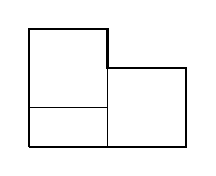
\begin{tikzpicture}[x=0.5cm, y=0.5cm]
      \draw[thick] (1,1) -- (5,1) -- (5,3) -- (3,3) -- (3,4) -- (1,4) -- (1,1);
      \draw (1,2) -- (3,2);
      \draw (3,1) -- (3,3);
  \end{tikzpicture}}
  \hfill
  \subcaptionbox{}
  {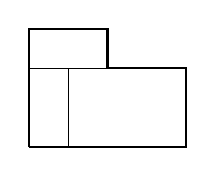
\begin{tikzpicture}[x=0.5cm, y=0.5cm]
      \draw[thick] (1,1) -- (5,1) -- (5,3) -- (3,3) -- (3,4) -- (1,4) -- (1,1);
      \draw (1,3) -- (3,3);
      \draw (2,1) -- (2,3);
  \end{tikzpicture}}
  \hfill
  \subcaptionbox{}
  {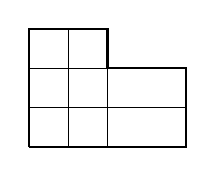
\begin{tikzpicture}[x=0.5cm, y=0.5cm]
      \draw[thick] (1,1) -- (5,1) -- (5,3) -- (3,3) -- (3,4) -- (1,4) -- (1,1);
      \draw (1,2) -- (5,2);
      \draw (1,3) -- (3,3);
      \draw (2,1) -- (2,4);
      \draw (3,1) -- (3,4);
  \end{tikzpicture}}
  \hfill\mbox{}
  \caption{Lo stesso polirettangolo si può ottenere
  come due diverse unioni di rettangoli: (a), (b). Prendendo in considerazione
  tutte le rette che contengono i lati di tutti i rettangoli coinvolti si
  ottiene una suddivisione (c) per cui ogni rettangolo in (a) o in (b) è unione di rettangoli in (c).}
\end{figure}

Per lo stesso motivo risulta chiaro che se $E$ e $F$ sono due polirettangoli
anche $E\cup F$, $E \cap F$, $E\setminus F$  e $F\setminus E$ sono polirettangoli e risulta
\begin{equation}\label{eq:48474624}
  m(E \cup F) = m(E\setminus F) + m(E\cap F) + m(F\setminus E).
\end{equation}
Infatti è possibile trovare una famiglia di rettangolini (quelli identificati
dalla griglia di tutte le rette contenenti i lati dei rettangoli di $E$ e dei rettangoli di $F$)
che sono tra loro disgiunti e tali che
$E\cap F$, $E\setminus F$ e $F\setminus E$
possono essere scritti come unione di questi rettangolini. Questi insiemi
sono tra loro disgiunti e quindi, scrivendo l'area di ognuno come la somma delle
aree dei rettangoli, si trova~\eqref{eq:48474624}.

Se ora prendiamo un insieme $E\subset \RR^2$ qualunque
e imponiamo che valga la proprietà di monotonia,
dovremo avere che $m(E)$, se è definibile, deve
essere l'elemento di separazione tra le misure
dei polirettangoli contenuti in $E$ e di quelli contenenti $E$.
Si giustifica quindi la seguente.

\begin{definition}[misura di Peano-Jordan]
\label{def:peano-jordan}%
\mymargin{Peano-Jordan}%
\index{misura!di Peano-Jordan}%
\index{Peano-Jordan!misura di}%
\index{Jordan!misura di}%
Sia $E\subset \RR^2$ un insieme limitato. Definiamo:
\begin{align*}
m^*(E) &= \inf\ENCLOSE{m(F)\colon \text{$F\supset E$, $F$ polirettangolo}}, \\
m_*(E) &= \sup\ENCLOSE{m(F)\colon \text{$F\subset E$, $F$ polirettangolo}}.
\end{align*}

Visto che $E$ è limitato (dunque è contenuto in un rettangolo limitato)
si ha $m^*(E)<+\infty$ e visto che $\emptyset \subset E$
e $m(\emptyset)=0$ (l'insieme vuoto $\emptyset = (a,a) \times (c,c)$ è un
polirettangolo di area nulla) si ha $m_*(E)\ge 0$. Inoltre $m_*(E)\le m^*(E)$
in quanto ogni polirettangolo contenuto in $E$ è contenuto, e quindi ha area non superiore, 
ad ogni polirettangolo contenente $E$.

Se $m^*(E) = m_*(E)$ diciamo che $E$ è \myemph{misurabile} secondo Peano-Jordan
e poniamo $m(E) = m^*(E) = m_*(E)$ la sua misura di Peano-Jordan.
\end{definition}

\begin{theorem}[proprietà della misura di Peano-Jordan]
Se $E$ e $F$ sono Peano-Jordan misurabili allora anche
$E\cup F$, $E\setminus F$, $F\setminus E$, $E\cap F$
sono Peano-Jordan misurabili e risulta
\begin{align*}
  m(E\cup F)
  &= m(E\setminus F) + m(E\cap F) + m(F\setminus E)\\
  &= m(E) + m(F) - m(E\cap F).
\end{align*}
\end{theorem}
%
\begin{proof}
Osserviamo che un insieme $E$ è misurabile se e solo se
per ogni $\eps>0$ esistono dei polirettangoli $E_*, E^*$
con $E_* \subset E \subset E^*$ tali che $m(E^*)-m(E_*)<\eps$
(basta utilizzare la caratterizzazione di estremo superiore e inferiore).

\begin{figure}
  \centering\ifdefined\figurePJA

\begin{tikzpicture}[x=0.5cm, y=0.5cm]
  \draw[draw=none,fill=white] (0,0) -- (14,00) -- (14,10) -- (0,10) -- (0,0);
\draw[fill=black,draw=none] plot [smooth cycle] coordinates {(1,4) (5,3) (7,1) (9,5) (5,8) (1,6)};
\end{tikzpicture}
\else
\ifdefined\figurePJB
%% draw set B

\begin{tikzpicture}[x=0.5cm, y=0.5cm]
\draw[draw=none,fill=white] (0,0) -- (14,00) -- (14,10) -- (0,10) -- (0,0);
\draw[fill=black,draw=none] plot [smooth cycle] coordinates {(10,1) (13,4) (10,8) (6,4)};
\end{tikzpicture}
\else
%
\begin{tikzpicture}[x=0.5cm, y=0.5cm]
  % False
% 255 255 255
\draw[draw=red] 
(4.05,7.94)--(3.85,7.94)--(3.65,7.94)--(3.65,7.77)--(3.45,7.77)--(3.24,7.77)--(3.24,7.6)--(3.04,7.6)--(2.84,7.6)--(2.84,7.43)--(2.64,7.43)--(2.64,7.26)--(2.43,7.26)--(2.23,7.26)--(2.23,7.09)--(2.03,7.09)--(2.03,6.93)--(1.82,6.93)--(1.82,6.76)--(1.62,6.76)--(1.62,6.59)--(1.42,6.59)--(1.22,6.59)--(1.22,6.42)--(1.01,6.42)--(1.01,6.25)--(0.811,6.25)--(0.811,6.08)--(0.811,5.91)--(0.608,5.91)--(0.608,5.74)--(0.608,5.57)--(0.405,5.57)--(0.405,5.41)--(0.405,5.24)--(0.405,5.07)--(0.405,4.9)--(0.405,4.73)--(0.405,4.56)--(0.405,4.39)--(0.608,4.39)--(0.608,4.22)--(0.608,4.05)--(0.811,4.05)--(0.811,3.89)--(1.01,3.89)--(1.01,3.72)--(1.22,3.72)--(1.42,3.72)--(1.62,3.72)--(1.62,3.55)--(1.82,3.55)--(2.03,3.55)--(2.23,3.55)--(2.43,3.55)--(2.43,3.38)--(2.64,3.38)--(2.84,3.38)--(3.04,3.38)--(3.24,3.38)--(3.24,3.21)--(3.45,3.21)--(3.65,3.21)--(3.85,3.21)--(4.05,3.21)--(4.26,3.21)--(4.26,3.04)--(4.46,3.04)--(4.66,3.04)--(4.66,2.87)--(4.86,2.87)--(5.07,2.87)--(5.07,2.7)--(5.27,2.7)--(5.27,2.53)--(5.47,2.53)--(5.47,2.36)--(5.47,2.2)--(5.68,2.2)--(5.68,2.03)--(5.68,1.86)--(5.88,1.86)--(5.88,1.69)--(5.88,1.52)--(6.08,1.52)--(6.08,1.35)--(6.28,1.35)--(6.28,1.18)--(6.28,1.01)--(6.49,1.01)--(6.49,0.845)--(6.69,0.845)--(6.89,0.845)--(7.09,0.845)--(7.09,1.01)--(7.3,1.01)--(7.3,1.18)--(7.5,1.18)--(7.5,1.35)--(7.7,1.35)--(7.7,1.52)--(7.7,1.69)--(7.91,1.69)--(7.91,1.86)--(8.11,1.86)--(8.11,2.03)--(8.11,2.2)--(8.31,2.2)--(8.31,2.36)--(8.31,2.53)--(8.51,2.53)--(8.51,2.7)--(8.51,2.87)--(8.51,3.04)--(8.72,3.04)--(8.72,3.21)--(8.72,3.38)--(8.92,3.38)--(8.92,3.55)--(8.92,3.72)--(8.92,3.89)--(8.92,4.05)--(9.12,4.05)--(9.12,4.22)--(9.12,4.39)--(9.12,4.56)--(9.12,4.73)--(9.12,4.9)--(9.12,5.07)--(9.12,5.24)--(9.12,5.41)--(8.92,5.41)--(8.92,5.57)--(8.72,5.57)--(8.72,5.74)--(8.72,5.91)--(8.51,5.91)--(8.51,6.08)--(8.31,6.08)--(8.31,6.25)--(8.11,6.25)--(8.11,6.42)--(7.91,6.42)--(7.91,6.59)--(7.7,6.59)--(7.7,6.76)--(7.5,6.76)--(7.5,6.93)--(7.3,6.93)--(7.3,7.09)--(7.09,7.09)--(7.09,7.26)--(6.89,7.26)--(6.89,7.43)--(6.69,7.43)--(6.49,7.43)--(6.49,7.6)--(6.28,7.6)--(6.28,7.77)--(6.08,7.77)--(5.88,7.77)--(5.88,7.94)--(5.68,7.94)--(5.47,7.94)--(5.47,8.11)--(5.27,8.11)--(5.07,8.11)--(4.86,8.11)--(4.66,8.11)--(4.46,8.11)--(4.26,8.11)--(4.05,8.11)--(4.05,7.94)
;
\begin{scope}[on background layer]
\draw[draw=none,fill=red!10] 
(4.05,7.94)--(3.85,7.94)--(3.65,7.94)--(3.65,7.77)--(3.45,7.77)--(3.24,7.77)--(3.24,7.6)--(3.04,7.6)--(2.84,7.6)--(2.84,7.43)--(2.64,7.43)--(2.64,7.26)--(2.43,7.26)--(2.23,7.26)--(2.23,7.09)--(2.03,7.09)--(2.03,6.93)--(1.82,6.93)--(1.82,6.76)--(1.62,6.76)--(1.62,6.59)--(1.42,6.59)--(1.22,6.59)--(1.22,6.42)--(1.01,6.42)--(1.01,6.25)--(0.811,6.25)--(0.811,6.08)--(0.811,5.91)--(0.608,5.91)--(0.608,5.74)--(0.608,5.57)--(0.405,5.57)--(0.405,5.41)--(0.405,5.24)--(0.405,5.07)--(0.405,4.9)--(0.405,4.73)--(0.405,4.56)--(0.405,4.39)--(0.608,4.39)--(0.608,4.22)--(0.608,4.05)--(0.811,4.05)--(0.811,3.89)--(1.01,3.89)--(1.01,3.72)--(1.22,3.72)--(1.42,3.72)--(1.62,3.72)--(1.62,3.55)--(1.82,3.55)--(2.03,3.55)--(2.23,3.55)--(2.43,3.55)--(2.43,3.38)--(2.64,3.38)--(2.84,3.38)--(3.04,3.38)--(3.24,3.38)--(3.24,3.21)--(3.45,3.21)--(3.65,3.21)--(3.85,3.21)--(4.05,3.21)--(4.26,3.21)--(4.26,3.04)--(4.46,3.04)--(4.66,3.04)--(4.66,2.87)--(4.86,2.87)--(5.07,2.87)--(5.07,2.7)--(5.27,2.7)--(5.27,2.53)--(5.47,2.53)--(5.47,2.36)--(5.47,2.2)--(5.68,2.2)--(5.68,2.03)--(5.68,1.86)--(5.88,1.86)--(5.88,1.69)--(5.88,1.52)--(6.08,1.52)--(6.08,1.35)--(6.28,1.35)--(6.28,1.18)--(6.28,1.01)--(6.49,1.01)--(6.49,0.845)--(6.69,0.845)--(6.89,0.845)--(7.09,0.845)--(7.09,1.01)--(7.3,1.01)--(7.3,1.18)--(7.5,1.18)--(7.5,1.35)--(7.7,1.35)--(7.7,1.52)--(7.7,1.69)--(7.91,1.69)--(7.91,1.86)--(8.11,1.86)--(8.11,2.03)--(8.11,2.2)--(8.31,2.2)--(8.31,2.36)--(8.31,2.53)--(8.51,2.53)--(8.51,2.7)--(8.51,2.87)--(8.51,3.04)--(8.72,3.04)--(8.72,3.21)--(8.72,3.38)--(8.92,3.38)--(8.92,3.55)--(8.92,3.72)--(8.92,3.89)--(8.92,4.05)--(9.12,4.05)--(9.12,4.22)--(9.12,4.39)--(9.12,4.56)--(9.12,4.73)--(9.12,4.9)--(9.12,5.07)--(9.12,5.24)--(9.12,5.41)--(8.92,5.41)--(8.92,5.57)--(8.72,5.57)--(8.72,5.74)--(8.72,5.91)--(8.51,5.91)--(8.51,6.08)--(8.31,6.08)--(8.31,6.25)--(8.11,6.25)--(8.11,6.42)--(7.91,6.42)--(7.91,6.59)--(7.7,6.59)--(7.7,6.76)--(7.5,6.76)--(7.5,6.93)--(7.3,6.93)--(7.3,7.09)--(7.09,7.09)--(7.09,7.26)--(6.89,7.26)--(6.89,7.43)--(6.69,7.43)--(6.49,7.43)--(6.49,7.6)--(6.28,7.6)--(6.28,7.77)--(6.08,7.77)--(5.88,7.77)--(5.88,7.94)--(5.68,7.94)--(5.47,7.94)--(5.47,8.11)--(5.27,8.11)--(5.07,8.11)--(4.86,8.11)--(4.66,8.11)--(4.46,8.11)--(4.26,8.11)--(4.05,8.11)--(4.05,7.94)
;
\end{scope}

  % False
% 255 255 255
\draw[draw=red] 
(9.46,7.91)--(9.22,7.91)--(8.99,7.91)--(8.99,7.7)--(8.75,7.7)--(8.75,7.5)--(8.51,7.5)--(8.51,7.3)--(8.28,7.3)--(8.28,7.09)--(8.04,7.09)--(8.04,6.89)--(7.8,6.89)--(7.8,6.69)--(7.57,6.69)--(7.57,6.49)--(7.33,6.49)--(7.33,6.28)--(7.09,6.28)--(7.09,6.08)--(6.86,6.08)--(6.86,5.88)--(6.86,5.68)--(6.62,5.68)--(6.62,5.47)--(6.39,5.47)--(6.39,5.27)--(6.39,5.07)--(6.15,5.07)--(6.15,4.86)--(6.15,4.66)--(5.91,4.66)--(5.91,4.46)--(5.91,4.26)--(5.91,4.05)--(5.91,3.85)--(5.91,3.65)--(5.91,3.45)--(6.15,3.45)--(6.15,3.24)--(6.15,3.04)--(6.39,3.04)--(6.39,2.84)--(6.62,2.84)--(6.62,2.64)--(6.86,2.64)--(6.86,2.43)--(7.09,2.43)--(7.09,2.23)--(7.33,2.23)--(7.33,2.03)--(7.57,2.03)--(7.57,1.82)--(7.8,1.82)--(7.8,1.62)--(8.04,1.62)--(8.28,1.62)--(8.28,1.42)--(8.51,1.42)--(8.51,1.22)--(8.75,1.22)--(8.99,1.22)--(8.99,1.01)--(9.22,1.01)--(9.46,1.01)--(9.7,1.01)--(9.7,0.811)--(9.93,0.811)--(10.2,0.811)--(10.4,0.811)--(10.4,1.01)--(10.6,1.01)--(10.9,1.01)--(10.9,1.22)--(11.1,1.22)--(11.1,1.42)--(11.4,1.42)--(11.4,1.62)--(11.6,1.62)--(11.6,1.82)--(11.8,1.82)--(11.8,2.03)--(12.1,2.03)--(12.1,2.23)--(12.3,2.23)--(12.3,2.43)--(12.5,2.43)--(12.5,2.64)--(12.5,2.84)--(12.8,2.84)--(12.8,3.04)--(12.8,3.24)--(13.0,3.24)--(13.0,3.45)--(13.0,3.65)--(13.0,3.85)--(13.0,4.05)--(13.0,4.26)--(13.0,4.46)--(13.0,4.66)--(13.0,4.86)--(13.0,5.07)--(12.8,5.07)--(12.8,5.27)--(12.8,5.47)--(12.5,5.47)--(12.5,5.68)--(12.5,5.88)--(12.3,5.88)--(12.3,6.08)--(12.3,6.28)--(12.1,6.28)--(12.1,6.49)--(11.8,6.49)--(11.8,6.69)--(11.8,6.89)--(11.6,6.89)--(11.6,7.09)--(11.4,7.09)--(11.4,7.3)--(11.4,7.5)--(11.1,7.5)--(11.1,7.7)--(10.9,7.7)--(10.9,7.91)--(10.6,7.91)--(10.6,8.11)--(10.4,8.11)--(10.2,8.11)--(9.93,8.11)--(9.7,8.11)--(9.46,8.11)--(9.46,7.91)
;
\begin{scope}[on background layer]
\draw[draw=none,fill=red!10] 
(9.46,7.91)--(9.22,7.91)--(8.99,7.91)--(8.99,7.7)--(8.75,7.7)--(8.75,7.5)--(8.51,7.5)--(8.51,7.3)--(8.28,7.3)--(8.28,7.09)--(8.04,7.09)--(8.04,6.89)--(7.8,6.89)--(7.8,6.69)--(7.57,6.69)--(7.57,6.49)--(7.33,6.49)--(7.33,6.28)--(7.09,6.28)--(7.09,6.08)--(6.86,6.08)--(6.86,5.88)--(6.86,5.68)--(6.62,5.68)--(6.62,5.47)--(6.39,5.47)--(6.39,5.27)--(6.39,5.07)--(6.15,5.07)--(6.15,4.86)--(6.15,4.66)--(5.91,4.66)--(5.91,4.46)--(5.91,4.26)--(5.91,4.05)--(5.91,3.85)--(5.91,3.65)--(5.91,3.45)--(6.15,3.45)--(6.15,3.24)--(6.15,3.04)--(6.39,3.04)--(6.39,2.84)--(6.62,2.84)--(6.62,2.64)--(6.86,2.64)--(6.86,2.43)--(7.09,2.43)--(7.09,2.23)--(7.33,2.23)--(7.33,2.03)--(7.57,2.03)--(7.57,1.82)--(7.8,1.82)--(7.8,1.62)--(8.04,1.62)--(8.28,1.62)--(8.28,1.42)--(8.51,1.42)--(8.51,1.22)--(8.75,1.22)--(8.99,1.22)--(8.99,1.01)--(9.22,1.01)--(9.46,1.01)--(9.7,1.01)--(9.7,0.811)--(9.93,0.811)--(10.2,0.811)--(10.4,0.811)--(10.4,1.01)--(10.6,1.01)--(10.9,1.01)--(10.9,1.22)--(11.1,1.22)--(11.1,1.42)--(11.4,1.42)--(11.4,1.62)--(11.6,1.62)--(11.6,1.82)--(11.8,1.82)--(11.8,2.03)--(12.1,2.03)--(12.1,2.23)--(12.3,2.23)--(12.3,2.43)--(12.5,2.43)--(12.5,2.64)--(12.5,2.84)--(12.8,2.84)--(12.8,3.04)--(12.8,3.24)--(13.0,3.24)--(13.0,3.45)--(13.0,3.65)--(13.0,3.85)--(13.0,4.05)--(13.0,4.26)--(13.0,4.46)--(13.0,4.66)--(13.0,4.86)--(13.0,5.07)--(12.8,5.07)--(12.8,5.27)--(12.8,5.47)--(12.5,5.47)--(12.5,5.68)--(12.5,5.88)--(12.3,5.88)--(12.3,6.08)--(12.3,6.28)--(12.1,6.28)--(12.1,6.49)--(11.8,6.49)--(11.8,6.69)--(11.8,6.89)--(11.6,6.89)--(11.6,7.09)--(11.4,7.09)--(11.4,7.3)--(11.4,7.5)--(11.1,7.5)--(11.1,7.7)--(10.9,7.7)--(10.9,7.91)--(10.6,7.91)--(10.6,8.11)--(10.4,8.11)--(10.2,8.11)--(9.93,8.11)--(9.7,8.11)--(9.46,8.11)--(9.46,7.91)
;
\end{scope}

  % True
% 255 255 255
\draw[draw=blue] 
(4.46,7.77)--(4.26,7.77)--(4.05,7.77)--(3.85,7.77)--(3.85,7.6)--(3.65,7.6)--(3.45,7.6)--(3.45,7.43)--(3.24,7.43)--(3.24,7.26)--(3.04,7.26)--(2.84,7.26)--(2.84,7.09)--(2.64,7.09)--(2.64,6.93)--(2.43,6.93)--(2.23,6.93)--(2.23,6.76)--(2.03,6.76)--(2.03,6.59)--(1.82,6.59)--(1.82,6.42)--(1.62,6.42)--(1.62,6.25)--(1.42,6.25)--(1.42,6.08)--(1.22,6.08)--(1.22,5.91)--(1.01,5.91)--(1.01,5.74)--(0.811,5.74)--(0.811,5.57)--(0.811,5.41)--(0.811,5.24)--(0.608,5.24)--(0.608,5.07)--(0.608,4.9)--(0.608,4.73)--(0.811,4.73)--(0.811,4.56)--(0.811,4.39)--(0.811,4.22)--(1.01,4.22)--(1.01,4.05)--(1.22,4.05)--(1.42,4.05)--(1.42,3.89)--(1.62,3.89)--(1.82,3.89)--(2.03,3.89)--(2.03,3.72)--(2.23,3.72)--(2.43,3.72)--(2.64,3.72)--(2.84,3.72)--(2.84,3.55)--(3.04,3.55)--(3.24,3.55)--(3.45,3.55)--(3.65,3.55)--(3.85,3.55)--(3.85,3.38)--(4.05,3.38)--(4.26,3.38)--(4.46,3.38)--(4.46,3.21)--(4.66,3.21)--(4.86,3.21)--(5.07,3.21)--(5.07,3.04)--(5.27,3.04)--(5.27,2.87)--(5.47,2.87)--(5.47,2.7)--(5.68,2.7)--(5.68,2.53)--(5.68,2.36)--(5.88,2.36)--(5.88,2.2)--(6.08,2.2)--(6.08,2.03)--(6.08,1.86)--(6.28,1.86)--(6.28,1.69)--(6.28,1.52)--(6.49,1.52)--(6.49,1.35)--(6.69,1.35)--(6.69,1.18)--(6.89,1.18)--(7.09,1.18)--(7.09,1.35)--(7.3,1.35)--(7.3,1.52)--(7.3,1.69)--(7.5,1.69)--(7.5,1.86)--(7.7,1.86)--(7.7,2.03)--(7.7,2.2)--(7.91,2.2)--(7.91,2.36)--(7.91,2.53)--(8.11,2.53)--(8.11,2.7)--(8.11,2.87)--(8.31,2.87)--(8.31,3.04)--(8.31,3.21)--(8.51,3.21)--(8.51,3.38)--(8.51,3.55)--(8.51,3.72)--(8.72,3.72)--(8.72,3.89)--(8.72,4.05)--(8.72,4.22)--(8.92,4.22)--(8.92,4.39)--(8.92,4.56)--(8.92,4.73)--(8.92,4.9)--(8.92,5.07)--(8.72,5.07)--(8.72,5.24)--(8.72,5.41)--(8.51,5.41)--(8.51,5.57)--(8.31,5.57)--(8.31,5.74)--(8.31,5.91)--(8.11,5.91)--(8.11,6.08)--(7.91,6.08)--(7.91,6.25)--(7.7,6.25)--(7.7,6.42)--(7.5,6.42)--(7.5,6.59)--(7.3,6.59)--(7.3,6.76)--(7.09,6.76)--(7.09,6.93)--(6.89,6.93)--(6.89,7.09)--(6.69,7.09)--(6.49,7.09)--(6.49,7.26)--(6.28,7.26)--(6.28,7.43)--(6.08,7.43)--(5.88,7.43)--(5.88,7.6)--(5.68,7.6)--(5.68,7.77)--(5.47,7.77)--(5.27,7.77)--(5.27,7.94)--(5.07,7.94)--(4.86,7.94)--(4.66,7.94)--(4.46,7.94)--(4.46,7.77)
;
\begin{scope}[on background layer]
\draw[draw=none,fill=blue!10] 
(4.46,7.77)--(4.26,7.77)--(4.05,7.77)--(3.85,7.77)--(3.85,7.6)--(3.65,7.6)--(3.45,7.6)--(3.45,7.43)--(3.24,7.43)--(3.24,7.26)--(3.04,7.26)--(2.84,7.26)--(2.84,7.09)--(2.64,7.09)--(2.64,6.93)--(2.43,6.93)--(2.23,6.93)--(2.23,6.76)--(2.03,6.76)--(2.03,6.59)--(1.82,6.59)--(1.82,6.42)--(1.62,6.42)--(1.62,6.25)--(1.42,6.25)--(1.42,6.08)--(1.22,6.08)--(1.22,5.91)--(1.01,5.91)--(1.01,5.74)--(0.811,5.74)--(0.811,5.57)--(0.811,5.41)--(0.811,5.24)--(0.608,5.24)--(0.608,5.07)--(0.608,4.9)--(0.608,4.73)--(0.811,4.73)--(0.811,4.56)--(0.811,4.39)--(0.811,4.22)--(1.01,4.22)--(1.01,4.05)--(1.22,4.05)--(1.42,4.05)--(1.42,3.89)--(1.62,3.89)--(1.82,3.89)--(2.03,3.89)--(2.03,3.72)--(2.23,3.72)--(2.43,3.72)--(2.64,3.72)--(2.84,3.72)--(2.84,3.55)--(3.04,3.55)--(3.24,3.55)--(3.45,3.55)--(3.65,3.55)--(3.85,3.55)--(3.85,3.38)--(4.05,3.38)--(4.26,3.38)--(4.46,3.38)--(4.46,3.21)--(4.66,3.21)--(4.86,3.21)--(5.07,3.21)--(5.07,3.04)--(5.27,3.04)--(5.27,2.87)--(5.47,2.87)--(5.47,2.7)--(5.68,2.7)--(5.68,2.53)--(5.68,2.36)--(5.88,2.36)--(5.88,2.2)--(6.08,2.2)--(6.08,2.03)--(6.08,1.86)--(6.28,1.86)--(6.28,1.69)--(6.28,1.52)--(6.49,1.52)--(6.49,1.35)--(6.69,1.35)--(6.69,1.18)--(6.89,1.18)--(7.09,1.18)--(7.09,1.35)--(7.3,1.35)--(7.3,1.52)--(7.3,1.69)--(7.5,1.69)--(7.5,1.86)--(7.7,1.86)--(7.7,2.03)--(7.7,2.2)--(7.91,2.2)--(7.91,2.36)--(7.91,2.53)--(8.11,2.53)--(8.11,2.7)--(8.11,2.87)--(8.31,2.87)--(8.31,3.04)--(8.31,3.21)--(8.51,3.21)--(8.51,3.38)--(8.51,3.55)--(8.51,3.72)--(8.72,3.72)--(8.72,3.89)--(8.72,4.05)--(8.72,4.22)--(8.92,4.22)--(8.92,4.39)--(8.92,4.56)--(8.92,4.73)--(8.92,4.9)--(8.92,5.07)--(8.72,5.07)--(8.72,5.24)--(8.72,5.41)--(8.51,5.41)--(8.51,5.57)--(8.31,5.57)--(8.31,5.74)--(8.31,5.91)--(8.11,5.91)--(8.11,6.08)--(7.91,6.08)--(7.91,6.25)--(7.7,6.25)--(7.7,6.42)--(7.5,6.42)--(7.5,6.59)--(7.3,6.59)--(7.3,6.76)--(7.09,6.76)--(7.09,6.93)--(6.89,6.93)--(6.89,7.09)--(6.69,7.09)--(6.49,7.09)--(6.49,7.26)--(6.28,7.26)--(6.28,7.43)--(6.08,7.43)--(5.88,7.43)--(5.88,7.6)--(5.68,7.6)--(5.68,7.77)--(5.47,7.77)--(5.27,7.77)--(5.27,7.94)--(5.07,7.94)--(4.86,7.94)--(4.66,7.94)--(4.46,7.94)--(4.46,7.77)
;
\end{scope}

  % True
% 255 255 255
\draw[draw=blue] 
(9.7,7.7)--(9.46,7.7)--(9.22,7.7)--(9.22,7.5)--(8.99,7.5)--(8.99,7.3)--(8.75,7.3)--(8.75,7.09)--(8.51,7.09)--(8.51,6.89)--(8.28,6.89)--(8.28,6.69)--(8.04,6.69)--(8.04,6.49)--(7.8,6.49)--(7.8,6.28)--(7.57,6.28)--(7.57,6.08)--(7.57,5.88)--(7.33,5.88)--(7.33,5.68)--(7.09,5.68)--(7.09,5.47)--(6.86,5.47)--(6.86,5.27)--(6.86,5.07)--(6.62,5.07)--(6.62,4.86)--(6.39,4.86)--(6.39,4.66)--(6.39,4.46)--(6.15,4.46)--(6.15,4.26)--(6.15,4.05)--(6.15,3.85)--(6.15,3.65)--(6.39,3.65)--(6.39,3.45)--(6.39,3.24)--(6.62,3.24)--(6.62,3.04)--(6.86,3.04)--(6.86,2.84)--(7.09,2.84)--(7.09,2.64)--(7.33,2.64)--(7.33,2.43)--(7.57,2.43)--(7.57,2.23)--(7.8,2.23)--(7.8,2.03)--(8.04,2.03)--(8.28,2.03)--(8.28,1.82)--(8.51,1.82)--(8.51,1.62)--(8.75,1.62)--(8.99,1.62)--(8.99,1.42)--(9.22,1.42)--(9.46,1.42)--(9.46,1.22)--(9.7,1.22)--(9.93,1.22)--(10.2,1.22)--(10.4,1.22)--(10.4,1.42)--(10.6,1.42)--(10.9,1.42)--(10.9,1.62)--(11.1,1.62)--(11.1,1.82)--(11.4,1.82)--(11.4,2.03)--(11.6,2.03)--(11.6,2.23)--(11.8,2.23)--(11.8,2.43)--(12.1,2.43)--(12.1,2.64)--(12.1,2.84)--(12.3,2.84)--(12.3,3.04)--(12.5,3.04)--(12.5,3.24)--(12.5,3.45)--(12.8,3.45)--(12.8,3.65)--(12.8,3.85)--(12.8,4.05)--(12.8,4.26)--(12.8,4.46)--(12.8,4.66)--(12.5,4.66)--(12.5,4.86)--(12.5,5.07)--(12.3,5.07)--(12.3,5.27)--(12.3,5.47)--(12.1,5.47)--(12.1,5.68)--(12.1,5.88)--(11.8,5.88)--(11.8,6.08)--(11.8,6.28)--(11.6,6.28)--(11.6,6.49)--(11.6,6.69)--(11.4,6.69)--(11.4,6.89)--(11.1,6.89)--(11.1,7.09)--(10.9,7.09)--(10.9,7.3)--(10.6,7.3)--(10.6,7.5)--(10.4,7.5)--(10.4,7.7)--(10.2,7.7)--(10.2,7.91)--(9.93,7.91)--(9.7,7.91)--(9.7,7.7)
;
\begin{scope}[on background layer]
\draw[draw=none,fill=blue!10] 
(9.7,7.7)--(9.46,7.7)--(9.22,7.7)--(9.22,7.5)--(8.99,7.5)--(8.99,7.3)--(8.75,7.3)--(8.75,7.09)--(8.51,7.09)--(8.51,6.89)--(8.28,6.89)--(8.28,6.69)--(8.04,6.69)--(8.04,6.49)--(7.8,6.49)--(7.8,6.28)--(7.57,6.28)--(7.57,6.08)--(7.57,5.88)--(7.33,5.88)--(7.33,5.68)--(7.09,5.68)--(7.09,5.47)--(6.86,5.47)--(6.86,5.27)--(6.86,5.07)--(6.62,5.07)--(6.62,4.86)--(6.39,4.86)--(6.39,4.66)--(6.39,4.46)--(6.15,4.46)--(6.15,4.26)--(6.15,4.05)--(6.15,3.85)--(6.15,3.65)--(6.39,3.65)--(6.39,3.45)--(6.39,3.24)--(6.62,3.24)--(6.62,3.04)--(6.86,3.04)--(6.86,2.84)--(7.09,2.84)--(7.09,2.64)--(7.33,2.64)--(7.33,2.43)--(7.57,2.43)--(7.57,2.23)--(7.8,2.23)--(7.8,2.03)--(8.04,2.03)--(8.28,2.03)--(8.28,1.82)--(8.51,1.82)--(8.51,1.62)--(8.75,1.62)--(8.99,1.62)--(8.99,1.42)--(9.22,1.42)--(9.46,1.42)--(9.46,1.22)--(9.7,1.22)--(9.93,1.22)--(10.2,1.22)--(10.4,1.22)--(10.4,1.42)--(10.6,1.42)--(10.9,1.42)--(10.9,1.62)--(11.1,1.62)--(11.1,1.82)--(11.4,1.82)--(11.4,2.03)--(11.6,2.03)--(11.6,2.23)--(11.8,2.23)--(11.8,2.43)--(12.1,2.43)--(12.1,2.64)--(12.1,2.84)--(12.3,2.84)--(12.3,3.04)--(12.5,3.04)--(12.5,3.24)--(12.5,3.45)--(12.8,3.45)--(12.8,3.65)--(12.8,3.85)--(12.8,4.05)--(12.8,4.26)--(12.8,4.46)--(12.8,4.66)--(12.5,4.66)--(12.5,4.86)--(12.5,5.07)--(12.3,5.07)--(12.3,5.27)--(12.3,5.47)--(12.1,5.47)--(12.1,5.68)--(12.1,5.88)--(11.8,5.88)--(11.8,6.08)--(11.8,6.28)--(11.6,6.28)--(11.6,6.49)--(11.6,6.69)--(11.4,6.69)--(11.4,6.89)--(11.1,6.89)--(11.1,7.09)--(10.9,7.09)--(10.9,7.3)--(10.6,7.3)--(10.6,7.5)--(10.4,7.5)--(10.4,7.7)--(10.2,7.7)--(10.2,7.91)--(9.93,7.91)--(9.7,7.91)--(9.7,7.7)
;
\end{scope}

  \draw[thick] plot [smooth cycle] coordinates {(1,4) (5,3) (7,1) (9,5) (5,8) (1,6)};
  \draw[thick] plot [smooth cycle] coordinates {(10,1) (13,4) (10,8) (6,4)};
  \node at (4,5) {$E$};
  \node at (10,5) {$F$};
\end{tikzpicture}
\fi
\fi

  \caption{Gli insiemi $E$ ed $F$ e i polirettangoli approssimanti 
  dall'interno e dall'esterno. 
  Le approssimanti possono essere scelte in modo che la cornice tra 
  i polirettangoli esterni ed interni abbia area minore di un 
  qualunque $\eps>0$.}
  \label{fig:PeanoJordan}
\end{figure}
Dunque nelle nostre ipotesi per ogni
$\eps>0$ esistono dei polirettangoli $E^*$, $E_*$, $F^*$, $F_*$
tali che
\[
   E_* \subset E \subset E^*, \qquad
   F_* \subset F \subset F^*
\]
con
\[
  m(E^*)-m(E_*) < \eps,\qquad
  m(F^*)-m(F_*) < \eps.
\]
Possiamo allora approssimare gli insiemi $E\cap F$, $E\cup F$ e $E\setminus F$ dall'interno e dall'esterno con polirettangoli:
\begin{gather*}
  E_*\cap F_* \subset E\cap F \subset E^*\cap F^*, \\
  E_*\cup F_* \subset E\cup F \subset E^* \cup F^*, \\
  E_* \setminus F^* \subset E\setminus F \subset E^*\setminus F_*.
\end{gather*}
Le differenze tra gli approssimanti esterni e gli approssimanti
interni è sempre contenuta nell'unione
delle cornici $\Delta = (E^*\setminus E_*)\cup (F^*\setminus F_*)$
(si faccia riferimento alla figura~\ref{fig:PeanoJordan}):
\begin{align*}
  (E^*\cap F^*) \setminus (E_* \cap F_*) \subset \Delta \\
  (E^*\cup F^*) \setminus (E_*\cup F_*) \subset \Delta \\
  (E^*\setminus F_*) \setminus (E_* \setminus F^*) \subset \Delta
\end{align*}
e dunque essendo $m(\Delta)<2\eps$ ed essendo $\eps>0$ arbitrario
possiamo concludere che gli insiemi $E\cap F$, $E\cup F$ ed $E\setminus F$ sono misurabili.
Con le stesse considerazioni si può facilmente verificare
che l'unione dei polirettangoli disgiunti
$E_*\setminus F^*$ e $E_*\cap F_*$ differisce dal polirettangolo
$E_*$ per un insieme di misura minore di $\eps$ e dunque, passando al limite per $\eps\to 0$ si ottiene:
\[
  m(E\setminus F) + m(E\cap F) = m(E).
\]
Invertendo i ruoli di $E$ ed $F$ si ottiene che anche $F\setminus E$
è misurabile e vale la relazione analoga. Con considerazioni del
tutto simili si ottiene
\[
  m(E\cup F) = m(E) + m(F\setminus E).
\]
Di conseguenza si ottengono le uguaglianze enunciate nel teorema.
\end{proof}

\begin{theorem}[elemento d'area di una trasformazione lineare]
\label{th:area_lineare}%
\index{elemento!d'area}%
\index{misura!trasformazione lineare}%
Sia $E\subset \RR^2$ e sia $L\colon \RR^2\to\RR^2$ una trasformazione
lineare affine:
\[
  L(x,y) = M\cdot \begin{pmatrix}x \\ y\end{pmatrix}
  + \begin{pmatrix}x_0 \\ y_0\end{pmatrix}
\]
con $M$ matrice $2\times 2$ e $(x_0 ,y_0)\in \RR^2$.
Allora se $E$ è misurabile secondo Peano-Jordan anche $L(E)$ lo è.
E in tal caso si ha
\begin{equation}\label{eq:formula_area}
  m(L(E)) = \abs{\det M} \cdot m(E).
\end{equation}
\end{theorem}
%
\begin{proof}

Osserviamo innanzitutto che è sufficiente verificare
quello che succede nel caso in cui $E$ sia un rettangolo.
Infatti un generico insieme misurabile $E$ può essere approssimato,
per ogni $\eps>0$ con polirettangoli $E^\pm$ con $E^-\subset E \subset E^+$ e $m(E^+) - m(E^-) < \eps$.
Supponiamo che $R^+_k$, $k=1,\dots, N$ siano i rettangoli che compongono $E^+$ e $R^-_k$, $k=1,\dots, M$ siano i rettangoli che compongono $E^-$.
Se sappiamo che la trasformazione $L$ manda rettangoli in insiemi
misurabili e se sappiamo che sui rettangoli vale $m(L(R_k^\pm)) = c \cdot m(R_k^\pm)$
(per una qualche costante $c\ge 0$) allora si deduce che $L(R_k^+)$ può essere approssimato dall'esterno con un polirettangolo
$F_k^+$ in modo che risulti $m(F_k^+) - m(L(R_k^+)) < \eps/N$ mentre $L(R_k^-)$ può essere approssimato dall'interno con un polirettangolo $F_k^-$ in modo che si abbia $m(L(R_k^-))-m(F_k^-) < \eps/M$. Facendo l'unione $F^+ = F_1^+ \cup \dots \cup F_N^+$
e $F^- = F_1^- \cup \dots \cup F_M^-$ si ottengono dei polirettangoli tali che $F^- \subset L(E)\subset F^+$ e
$m(F^+) - m(F^-) < (c\cdot  m(E^+) + \eps) - (c \cdot m(E^-) -\eps)
< (c+1) \eps$. Essendo $\eps>0$ arbitrario si deduce
che $F=L(E)$ è misurabile e $m(L(E)) = c\cdot  m(E)$.


\emph{Passo 1.}
Supponiamo che sia
$L(x,y) = (\lambda x,\mu y)$  (una trasformazione lineare diagonale).
Se $E$ è un rettangolo $E=[x_1,x_2]\times[y_1,y_2]$
allora se $\lambda\ge 0$, $\mu\ge 0$ allora $L(E) = [\lambda x_1, \lambda x_2] \times [\mu y_1, \mu y_2]$
e chiaramente $m(L(E)) = \lambda (x_2-x_1) \mu (y_2-y_1) = \lambda \mu m(E)$. Visto che $\det L = \lambda \mu$ abbiamo ottenuto il risultato voluto.
Se $\lambda$ o $\mu$ hanno segno negativo
gli estremi degli intervalli si possono
scambiare e in tal caso si ottiene $m(L(E)) = \abs{\lambda}\abs{x_2-x_1} \cdot \abs{\mu} \cdot \abs{y_2-y_1}$ e quindi, come
voluto, $m(L(E))=\abs{\det L} \cdot m(E)$.

Una eventuale componente di traslazione $(x_0,y_0)$ non ha nessuna
rilevanza e non la considereremo mai nel seguito in quanto i rettangoli traslati mantengono la stessa misura.

\emph{Passo 2.}
Supponiamo che sia $L(x,y) = (y,x)$ (la riflessione rispetto alla retta $y=x$). Questa trasformazione ha matrice associata $M=\begin{pmatrix}0&1\\1&0\end{pmatrix}$ che ha determinante
$-1$. Analiticamente scambia tra loro le coordinate $x$ ed $y$.
E' quindi immediato verificare che i rettangoli vengono mandati
in rettangoli con base e altezza scambiata e dunque la misura di
Peano-Jordan (e la misurabilità) rimangono invariate.
Dunque il teorema è banalmente valido in questo caso.

\emph{Passo 3.}
Supponiamo che sia $E=[a,b]\times[c,d]$ e $L(x,q)=(x,mx+q)$
con $m\in \RR$ fissato
(stiamo utilizzando le coordinate $(x,q)$ nel dominio di $L$
e le coordianate $(x,y)$ nel codominio).
Allora
\[
  L(E) = \{(x,y)\in \RR^2\colon x\in[a,b], mx+c \le y \le mx+d\}
\]
è un parallelogramma. Supponiamo per fissare le idee che sia $m\ge 0$.
Per ogni $n\in \NN$ posso affettare l'insieme
$L(E)$ con le rette verticali $x_k = a+\frac{k}{n}(b-a)$ e posso
identificare i rettangoli, per $k=1,\dots, n$:
\begin{align*}
   R_{k,n}^-
   &= \{(x,y)\in \RR^2 \colon x\in [x_{k-1},x_k), y\in[m x_k+c,m x_{k-1}+d]\},
   \\
   R_{k,n}^+
   &= \{(x,y)\in \RR^2 \colon x\in [x_{k-1},x_k), y\in[m x_{k-1}+c,m x_k+d]\}.
\end{align*}
e i polirettangoli ottenuti mettendo insieme questi rettangoli:
\begin{align*}
  P^-_n &= R_{1,n}^- \cup R_{2,n}^- \cup \dots \cup R_{n,n}^-, \\
  P^+_n & = R_{1,n}^+ \cup R_{2,n}^+ \cup \dots \cup R_{n,n}^+.
\end{align*}
Per come li abbiamo costruiti si osserva che
\[
  P^-_n \subset L(A) \subset P^+_n.
\]
Ma è facile calcolare le misure di questi polirettangoli:
\begin{align*}
  m(P^-_n) &= \sum_{k=1}^n m(R_{k,n}^-)
          = \sum_{k=1}^n(x_k-x_{k-1})\cdot (d-c-m(x_k-x_{k-1}))\\
         &= \sum_{k=1}^n \frac {b-a} n \cdot \enclose{d-c-\frac{m}{n}}
          = (b-a)\cdot \enclose{d-c-\frac{m}{n}} \\
  m(P^+) &= \sum_{k=1}^n m(R_{k,n}^+) = \dots = (b-a)\cdot \enclose{d-c+\frac{m}{n}}
\end{align*}
ma visto che per $n\to +\infty$ si ha $m(P^-_n)\to (b-a)\cdot(d-c)$
e $m(P^+_n) \to (b-a)\cdot(d-c)$ e visto che si ha
\[
  m(P^-_n)\le m_*(L(A))\le m^*(L(E)) \le m(P^+_n)
\]
otteniamo che $L(E)$ è misurabile e $m(L(E)) = (b-a)\cdot(d-c) = m(E)$.
La matrice associata ad $L$ è $M=\begin{pmatrix}1 & 0 \\ m & 1 \end{pmatrix}$
e dunque $\det M = 1$. Abbiamo quindi trovato il risultato voluto.

\emph{Passo 4.}
Sia $L$ una qualunque applicazione lineare che si ottiene come
composizione delle applicazioni considerate in precedenza: 
$L= L_n\circ \dots  \circ L_2 \circ L_1$. 
Allora per quanto già visto sappiamo
che se $E$ è un qualunque insieme Peano-Jordan misurabile risulta
\[
L(E) = L_n(\dots(L_2(L_1(E)))\dots)
     = \abs{\det L_n} \cdots \abs{\det L_2} \cdot \abs{\det L_1} \cdot m(E)
\]
e dunque anche $L(E)$ è Peano-Jordan misurabile e visto che
\[
 \abs{\det L} = \abs{\det L_n} \cdots \abs{\det L_1}
\]
la formula~\eqref{eq:formula_area} è verificata.

\emph{Passo 5.}
Per concludere la dimostrazione è dunque sufficiente
verificare che ogni trasformazione lineare si può scrivere come composizione delle trasformazioni già considerate.
In generale il teorema può essere formulato in dimensione qualunque (in $\RR^n$ invece che $\RR^2$) 
e la dimostrazione procede esattamente nello stesso modo considerando solo trasformazioni che coinvolgono due coordinate. 
La trasformazione che scambia due coordinate (passo 2) è rappresentata da una matrice che se moltiplicata 
a sinistra di una matrice generica $M$ ne scambia le righe, se moltiplicata a destra ne scambia le colonne. 
La trasformazione del passo 3 se applicata a sinistra somma ad una riga il multiplo di un'altra riga, 
se applicata a destra somma ad una colonna il multiplo di un'altra colonna.
Tramite il metodo di riduzione di Gauss (riduzione completa) è possibile trasformare ogni matrice 
utilizzando solamente queste trasfromazioni in modo da mantenere invariato il modulo del determinante 
e rendere la matrice diagonale. A quel punto ci siamo ricondotti al passo 1.

Nel caso planare $n=2$ che stiamo considerando possiamo fare esplicitamente la riduzione di Gauss. 
Supponiamo che la trasformazione lineare $L$ sia associata ad una matrice generica:
\[
  M = \begin{pmatrix} a&b\\c&d\end{pmatrix}.
\]
A meno di scambiare righe e colonne possiamo supporre che sia $a\neq 0$ 
(se tutti gli elementi fossero nulli avremmo $M=0$ che è già in forma diagonale). 
Allora moltiplichiamo la seconda riga per un multiplo $m$ della prima in modo da annullare il termine $b$:
\[
\begin{pmatrix} 1&0\\m&1\end{pmatrix}\cdot
    \begin{pmatrix} a&b\\c&d\end{pmatrix}
  =
  \begin{pmatrix} a&b\\c+ma&d+mb\end{pmatrix}
\]
scegliendo $m=-\frac c a$
e ponendo $d'=d+mb$
abbiamo ottenuto la matrice:
\[
\begin{pmatrix} a&b\\0&d'\end{pmatrix}.
\]
Ora osserviamo che
\[
      \begin{pmatrix} 0&1\\1&0\end{pmatrix}\cdot
      \begin{pmatrix} 1&0\\k&1\end{pmatrix}\cdot
      \begin{pmatrix} 0&1\\1&0\end{pmatrix}
      =
      \begin{pmatrix} 1&k\\0&1\end{pmatrix}\cdot
\]
Dunque possiamo utilizzare anche quest'ultima matrice
moltiplicandola a destra:
\[
\begin{pmatrix} a&b\\0&d'\end{pmatrix}\cdot
  \begin{pmatrix} 1&k\\0&1\end{pmatrix}
  =
  \begin{pmatrix} a&ak+b\\0&d'\end{pmatrix}
\]
dunque scegliendo $k=-\frac b a$ si ottiene finalmente
una matrice diagonale.
\end{proof}

\begin{comment}
\section{area di un poligono}

Il teorema~\ref{th:area_lineare} ci dice che se applichiamo ad un insieme 
$E$ una trasformazione lineare affine $L$ la cui matrice associata ha determinante 
$1$ o $-1$, otteniamo un insieme $L(E)$ con la stessa misura.
In particolare la misura di un insieme è invariante per isometrie:
cioè per quelle trasformazioni la cui matrice associata è ortogonale 
(traslazioni, rotazioni, riflessioni).

Se $E$ è un triangolo rettangolo con cateti di lunghezza $a$ e $b$ 
a meno di rotazioni e traslazioni possiamo supporre che $E$ si ottenga 
dividendo il rettangolo $[0,a]\times[0,b]$ lungo una diagonale. 
Visto che le due parti in cui il rettangolo viene suddiviso sono tra 
loro isometriche, esse devono avere ...

*** mi serve dimostrare che i poligoni sono misurabili ***
\end{comment}

L'integrale di Riemann, che andremo a definire
nella prossima sezione, ci permetterà di osservare che ogni figura geometrica
delimitata dal grafico di una curva sufficientemente regolare risulta
essere misurabile secondo Peano-Jordan. 
Inoltre il calcolo integrale ci permetterà
di determinare l'area di tali figure in modo piuttosto semplice.

\section{integrale di Riemann}

\begin{definition}[integrale di Riemann]
\mymark{***}
Siano $a,b\in \RR$, $a \le b$.
Un insieme $P\subset [a,b]$ si dice essere una \myemph{suddivisione di Riemann}
\index{Riemann!suddivisione di}
\index{partizione di Riemann}
\index{Riemann!partizione di}
dell'intervallo $[a,b]$ se $P$ è un insieme finito tale che $a,b\in P$.
In particolare $P$ si
potrà scrivere come
\[
 P = \ENCLOSE{ x_0, x_1, \dots, x_N}
\]
con
\[
  a = x_0 < x_1 < \dots < x_{N-1} < x_N = b.
\]

Sia $f\colon [a,b] \to \RR$ una funzione limitata.
Data una qualunque suddivisione $P$ di $[a,b]$ definiamo
rispettivamente le \emph{somme superiori} e le \emph{somme inferiori}
\mymargin{somme superiori/inferiori}
\index{Riemann!somme superiori}
\index{Riemann!somme inferiori}
come
\begin{align*}
S^*(f,P)
&= \sum_{k=1}^N (x_k - x_{k-1}) \cdot \sup f([x_{k-1},x_k]) \\
S_*(f,P)
&= \sum_{k=1}^N (x_k - x_{k-1}) \cdot \inf f([x_{k-1},x_k]).
\end{align*}
Definiamo infine
\begin{align*}
  I^*(f) &= \inf \ENCLOSE{S^*(f,P) \colon \text{$P$ suddivisione di $[a,b]$}}
  \\
  I_*(f) &= \sup \ENCLOSE{S_*(f,P) \colon \text{$P$ suddivisione di $[a,b]$}}.
\end{align*}

Se $I^*(f) = I_*(f)$ diremo che $f$ è
\emph{Riemann-integrabile}
\mymargin{integrale!di Riemann}%
\index{Riemann!integrale di}%
\index{integrabilità}%
\index{integrale}%
\index{integrale!definizione}%
e diremo che l'\emph{integrale} di $f$ su $[a,b]$ è
il valore comune $I^*(f)=I_*(f)$ che verrà denotato con
\[
  \int_a^b f
  \qquad{\text{oppure con}} \qquad
  \int_a^b f(x)\, dx.
\]

Se $b<a$ e se $f$ è Riemann integrabile su $[b,a]$
definiamo per convenzione:
\[
  \int_a^b f = -\int_b^a f.
\]
\end{definition}

\begin{lemma}
Sia $f\colon[a,b]\to \RR$ una funzione limitata.
Se $P$ e $Q$ sono due suddivisioni qualunque dell'intervallo
$[a,b]$ si ha
\begin{equation}\label{eq:5112309}
  S_*(f,P) \le S_*(f,P\cup Q)\le S^*(f,P\cup Q) \le S^*(f,Q).
\end{equation}
Di conseguenza $I_*(f) \le I^*(f)$.
\end{lemma}
\begin{proof}
  Sia $P$ una qualunque suddivisione di $[a,b]$ e sia $y\in [a,b]$ un punto qualunque. Posto $P' = P \cup \ENCLOSE{y}$ vogliamo mostrare
  che si ha
  \begin{equation}\label{eq:39543}
    S_*(f,P) \le S_*(f,P') \le S^*(f,P') \le S^*(f,P).
  \end{equation}
  Se $y\in P$ non c'è niente da dimostrare in quanto
  risulterebbe $P'=P$ e la disuguaglianza $S_*(f,P') \le S^*(f,P')$ è sempre verificata in quanto ogni estremo superiore che compare nella definizione di $S^*$ è maggiore o uguale al corrispondente
  estremo inferiore che compare nella definizione di $S_*$.
  Supponiamo allora che $y \not \in P$ e dunque che $y$ sia compreso tra due punti consecutivi $x_{k-1}, x_k$ della suddivisione $P$:
  \[
    a= x_0 < x_1 < \dots < x_{k-1} < y < x_k < \dots < x_N=b.
  \]
  Allora le somme che definiscono $S_*(f,P)$ e $S_*(f,P')$ 
  differiscono solo sull'intervallo $[x_{k-1},x_k]$. 
  % e si ha
  % \begin{align*}
  %   S_*(f,P') - S_*(f,P)
  %  &= (y-x_{k-1})\cdot \!\!\inf_{[x_{k-1},y]}\!\!\! f
  %  + (x_k - y)\cdot\! \inf_{[y,x_k]}\! f\\
  %  &\quad - (x_k - x_{k-1})\cdot \!\!\inf_{[x_{k-1}, x_k]}\!\!\!f
  % \end{align*}
  Ma osservando che
  \[
  \inf_{[x_{k-1}, x_k]}\!\!f
  \le\inf_{[x_{k-1},y]}\!\! f
  \qquad \text{e} \qquad
  \inf_{[x_{k-1}, x_k]}\!\!f
  \le\inf_{[y,x_k]}\!\! f
  \]
  si ottiene $S_*(f,P) \le S_*(f,P')$.
  In maniera analoga si ottiene $S^*(f,P) \ge S^*(f,P')$.
  Dunque \eqref{eq:39543} è dimostrata.
  Ma allora se $P$ e $Q$ sono suddivisioni qualunque osserviamo che $P\cup Q$ 
  si può ottenere da $P$ aggiungendo uno alla volta i punti di $Q$. 
  Iterando la \eqref{eq:39543} si ottiene \eqref{eq:5112309}.
  Facendo l'estremo inferiore al variare di $Q$
  si ottiene $S_*(f,P) \le I^*(f)$ e facendo l'estremo superiore al variare 
  di $P$ si ottiene $I_*(f) \le I^*(f)$.
  \end{proof}

\begin{theorem}[criteri di integrabilità]
\label{th:criteri_integrabilita}
\mymark{*}
\mynote{criteri di integrabilità}
\index{criterio!di integrabilità}
Sia $f\colon[a,b]\to \RR$ una funzione limitata.
\begin{enumerate}
\item
La funzione $f$ è Riemann-integrabile se e solo se
per ogni $\eps>0$ esiste una suddivisione $P$
tale che
\[
  S^*(f,P) - S_*(f,P) < \eps.
\]

\item
Se $f$ è Riemann-integrabile su $[a,b]$ allora
esiste una successione $P_n$ di suddivisioni tali che
\begin{equation}\label{eq:93765}
  \lim_{n\to +\infty} S^*(f,P_n)
  = \lim_{n\to+\infty} S_*(f,P_n)
  = \int_a^b f.
\end{equation}
Viceversa se $f$ è limitata ed esiste una successione $P_n$ 
di suddivisioni di $[a,b]$ per cui si ha
\begin{equation*}
  \lim_{n\to +\infty} \enclose{S^*(f,P_n) - S_*(f,P_n)} = 0
\end{equation*}
allora la funzione $f$ è Riemann-integrabile e vale~\eqref{eq:93765}.
\end{enumerate}
\end{theorem}
%
\begin{proof}
Se esiste una suddivisione $P$ tale che $S^*(f,P)-S_*(f,P) < \eps$ possiamo immediatamente concludere che
\[
I^*(f) - I_*(f) \le S^*(f,P) - S_*(f,P) < \eps.
\]
Se questo è vero per ogni $\eps >0$ deduciamo che $I^*(f) - I_*(f) = 0$ e dunque che $f$ è Riemann-integrabile.

Viceversa qualunque sia $f$, per le proprietà
di $\sup$ e $\inf$
esistono $Q$ e $R$ suddivisioni tali che
\[
  I^*(f) \ge S^*(f,Q) - \frac\eps 2
  \qquad\text{e}\qquad
  I_*(f) \le S_*(f,R) + \frac\eps 2
\]
da cui, per il lemma precedente, ponendo $P=Q\cup R$
se $f$ è Riemann integrabile
si ottiene
\begin{align*}
S^*(f,P)-S_*(f,P) &\le S^*(f,Q) - S_*(f,R) \\
&\le I^*(f) + \frac\eps 2 - \enclose{I_*(f) - \frac \eps 2} = \eps.
\end{align*}

Dimostriamo ora il secondo punto.
Supponiamo dapprima che $f$ sia Riemann-integrabile su $[a,b]$.
Allora per il punto precedente per ogni $n\in \NN$ ponendo $\eps=1/n$ possiamo trovare una suddivisione $P_n$ tale che
\[
  S^*(f,P_n) - S_*(f,P_n) < \frac 1 n
\]
da cui
\[
  I^*(f) \le S^*(f,P_n) \le S_*(f,P_n) + \frac 1 n
   \le I_*(f) + \frac 1 n
\]
perciò passando al limite per $n\to +\infty$,
essendo $I^*(f) = I_*(f) = \int_a^b f$ deve valere
\[
  \lim S^*(f,P_n) = \lim S_*(f,P_n) = \int_a^b f.
\]

Viceversa se
\[
 \lim_{n\to +\infty} S^*(f,P_n) - S_*(f,P_n) = 0
\]
per ogni $\eps>0$ esiste $n$ tale che
\[
  S^*(f,P_n) - S_*(f,P_n) < \eps.
\]
Per il punto precedente concludiamo che $f$ è Riemann-integrabile.
D'altra parte sappiamo che
\[
  S_*(f,P_n) \le I_*(f) = \int_a^b f = I^*(f) \le S^*(f,P_n)
\]
dunque se $S^*(f,P_n) - S_*(f,P_n) \to 0$ necessariamente
l'integrale coincide con i limiti di $S^*(f,P_n)$ e di
$S_*(f,P_n)$.
\end{proof}

\begin{example}[calcolo dell'integrale tramite le suddivisioni]
\label{ex:integrale_quadrato}
Mostriamo che per ogni $b>0$ la funzione $f(x)=x^2$ è Riemann-integrabile sull'intervallo $[0,b]$ e si ha
\[
 \int_0^b x^2\, dx = \frac{b^3}{3}.
\]
\end{example}
\begin{proof}
Consideriamo le suddivisioni \emph{equispaziate} dell'intervallo $[0,b]$, cioè dividiamo $[0,b]$ in $N$ intervalli ognuno di ampiezza $b/N$:
\[
P_N = \ENCLOSE{\frac{kb}{N}\colon k \in 0, 1, \dots, N}.
\]
Si ha
\[
  S^*(f,P_N) = \sum_{k=1}^N \sup_{[(k-1)b/N,kb/N]}f \cdot \frac b N
   = \frac{b}{N} \sum_{k=1}^N \frac{k^2b^2}{N^2}
   = \frac{b^3}{N^3} \sum_{k=1}^N k^2.
\]
Ricordiamo ora che vale
\[
  \sum_{k=1}^n k^2 = \frac{n(n+1)(2n+1)}{6} = \frac{2n^3+3n^2+n}{6}
\]
(tale formula può essere facilmente verificata per induzione). Dunque si ha
\[
  S^*(f,P_N) = \frac{b^3}{N^3} \frac{2N^3+3N^2+N}{6}
       = \frac{b^3}{6}\enclose{2 + \frac{3}{N}+\frac 1 N^2}
       \to \frac{b^3}{3}
\]
per $N\to +\infty$.
Analogamente si trova
\[
  S_*(f,P_N) = \sum_{k=1}^N \inf_{[(k-1)b/N,kb/N]} f \cdot \frac{b}{N}
  = \frac{b}{N}\sum_{k=1}^N \frac{(k-1)^2b^2}{N^2}
  = \frac{b^3}{N^3} \sum_{k=0}^{N-1} k^2
\]
e osservando che si ha
\[
 \sum_{k=0}^{N-1} k^2 = \sum_{k=1}^{N-1} k^2 = \frac{2(N-1)^3+3(N-2)^2+(N-1)}{6}
\]
otteniamo
\[
 S_*\ge \sup_N S_*(f,P_N) \ge \lim_{N\to+\infty} S_*(f,P_N) = \frac{b^3}{3} \to \frac{b^3}{3}.
\]
La dimostrazione si conclude quindi applicando
il criterio \eqref{eq:93765} del teorema precedente.
\end{proof}

\begin{theorem}[integrale della costante]
\label{th:integrale_costante}
Se $f\colon[a,b]\to \RR$ è costante: $f(x) = c$ allora
$f$ è Riemann-integrabile e si ha
\[
  \int_a^b f = c\cdot (b-a).
\]
\end{theorem}
%
\begin{proof}
Visto che su ogni $A\subset [a,b]$ si ha
\[
  \sup_A f = \inf_A f = c
\]
è facile verificare che si ha
\[
  S^*(f,P) = S_*(f,P) = c\cdot (b-a)
\]
qualunque sia la suddivisione $P$ di $[a,b]$. Il risultato segue immediatamente.
\end{proof}

Non tutte le funzioni sono Riemann-integrabili come ci mostra il seguente esempio.
\begin{example}[funzione di Dirichlet]
\mymark{**}
\mynote{funzione di Dirichlet}
\index{funzione!di Dirichlet}
\index{integrabilità!controesempio}
Sia $a<b$ e sia $f\colon[a,b]\to \RR$ la funzione definita da
\[
 f(x) =
 \begin{cases}
   1 & \text{se $x\in \QQ$}\\
   0 & \text{se $x\not \in \QQ$}.
 \end{cases}
\]
Allora $f$ non è Riemann-integrabile.
\end{example}
%
\begin{proof}
\mymark{*}
Sia $P=\ENCLOSE{x_0, x_1, \dots, x_N}$ con $a=x_0 < x_1 < \dots < x_N = b$
una qualunque suddivisione di $[a,b]$.
Allora basta osservare che, per la densità dei razionali,
in qualunque intervallino $I=[x_{k-1}, x_k]$ sono presenti infiniti punti
razionali e infiniti punti irrazionali. Dunque $\sup f(I)=1$ e $\inf f(I)=0$ e di conseguenza
\begin{align*}
  S^*(f,P) &= \sum_{k=1}^N (x_k - x_{k-1})\cdot 1 = b-a \\
  S_*(f,P) &= \sum_{k=1}^N (x_k - x_{k-1})\cdot 0 = 0
\end{align*}
da cui $I^*(f) = b-a \neq 0 = I_*(f)$.
\end{proof}

\begin{theorem}[monotonia dell'integrale]
\mymark{*}
Sia $a\le b$ e siano
$f,g\colon [a,b]\to \RR$ due funzioni Riemann-integrabili.
Se per ogni $x\in [a,b]$ si ha $f(x) \le g(x)$ allora
\[
  \int_a^b f(x) \le \int_a^b g(x).
\]

In particolare se $f\ge 0$ allora $\int_a^b f \ge 0$.
\end{theorem}
%
\begin{proof}
Chiaramente se $f \le g$ si avrà che il $\sup$ di $f$ su qualunque intervallo sarà minore o uguale al $\sup$ di $g$ sullo stesso intervallo. Dunque su ogni suddivisione $P$ di $[a,b]$ si avrà:
\[
  S^*(f,P) \le S^*(g,P)
\]
da cui si ottiene immediatamente $I^*(f) \le I^*(g)$ e il risultato segue.
\end{proof}

\begin{theorem}[linearità dell'integrale]
\mymark{*}
\label{th:integrale_lineare}
Siano $f,g\colon [a,b]\to \RR$ due funzioni Riemann-integrabili
e siano $\lambda, \mu \in \RR$. Allora $\lambda f + \mu g$
è Riemann integrabile e si ha
\[
  \int_a^b (\lambda f + \mu g) = \lambda \int_a^b f + \mu \int_a^b g.
\]

In particolare l'insieme delle funzioni Riemann-integrabili su $[a,b]$ risulta
essere uno spazio vettoriale reale e l'integrale è una
applicazione lineare su tale spazio, a valori in $\RR$.
\end{theorem}
%
\begin{proof}
\mymark{*}
Mostriamo innanzitutto che
\begin{equation}\label{eq:20043}
  \int_a^b (-f) = -\int_a^b f.
\end{equation}
Questo deriva dal fatto che su qualunque insieme $A$ si ha
$\sup_A (-f) = -\inf_A f$ e dunque per una qualunque suddivisione $P$
si ha
\[
  S^*(-f,P) = -S_*(f,P).
\]
Se ne deduce che $I^*(-f) = -I_*(f)$ e, analogamente, $I_*(-f) = -I^*(f)$.
Dunque se $f$ è Riemann-integrabile anche $-f$ lo è e vale la proprietà \eqref{eq:20043}.

Ora se $\lambda \ge 0$ vogliamo mostrare che vale
\begin{equation}\label{eq:10032}
  \int_a^b \lambda f = \lambda \int_a^b f.
\end{equation}
Semplicemente si osserva che $\sup_I \lambda f = \lambda \sup_I f$ e dunque
$S^*(\lambda f,P) = \lambda S^*(f,P)$ per ogni suddivisione $P$.
Ne consegue che $I^*(\lambda f) = \lambda I^*(f)$. In maniera analoga si può
mostrare che $I_*(\lambda f) = \lambda I_*(f)$. Dunque se $f$ è
Riemann-integrabile anche $\lambda f$ (con $\lambda \ge 0$) lo è e vale \eqref{eq:10032}.

Mettendo assieme \eqref{eq:20043} e $\eqref{eq:10032}$ si ottiene
che $\eqref{eq:10032}$ vale per ogni $\lambda \in \RR$.
Lo stesso sarà vero se mettiamo $g$ al posto di $f$ e $\mu$ al posto di $\lambda$.
Per concludere la dimostrazione sarà dunque sufficiente
mostrare che vale anche
\begin{equation*}\label{eq:80003}
\int_a^b (f+g) = \int_a^b f + \int_a^b g.
\end{equation*}
Osserviamo che su qualunque insieme $A$ si ha
\[
  \sup_A (f+g) \le \sup_A f + \sup_A g.
\]
Infatti per le proprietà dell'estremo superiore per ogni $\eps>0$ esiste $x\in A$ tale che
\[
  \sup_A (f+g) \le f(x) + g(x) + \eps.
\]
Ma chiaramente $f(x) \le \sup_A f$ e $g(x)\le \sup_A g$ dunque si ottiene
\[
  \sup_A (f+g) \le \sup_A f + \sup_A g + \eps.
\]
Passando al limite per $\eps \to 0^+$ si ottiene la disuguaglianza voluta.
Questo significa che
\[
  S^*(f+g) \le S^*(f) + S^*(g).
\]
analogamente si potrà dimostrare che
\[
  S_*(f+g) \ge S_*(f) + S_*(g).
\]
Si ottiene dunque
\[
  I^*(f+g) \le I^*(f) + I^*(g)
  \qquad\text{e}\qquad
  I_*(f+g) \ge I_*(f) + I_*(g)
\]
e dunque se $f$ e $g$ sono integrabili anche $f+g$ risulta integrabile
e vale la \eqref{eq:80003}.

Per concludere che l'insieme delle funzioni integrali sia uno spazio vettoriale
è sufficiente osservare che, grazie al teorema~\ref{th:integrale_costante},
la funzione $0$ risulta integrabile.
\end{proof}

\begin{theorem}[proprietà di reticolo]
\label{th:reticolo}%
Se $f$ e $g$ sono funzioni a valori reali definiamo le
funzioni $f\wedge g$ (minimo), $f \vee g$ (massimo),
$f^+$ (parte positiva) e $f^-$ (parte negativa) come segue:
\begin{gather*}
  (f \wedge g)(x) = \min\ENCLOSE{f(x), g(x)}  \qquad
  (f \vee g)(x) = \max\ENCLOSE{f(x), g(x)} \\
  f^+ (x) =
      \begin{cases}
      f(x) & \text{se $f(x)> 0$}\\
      0 & \text{altrimenti}
      \end{cases} \qquad
  f^- (x) =
      \begin{cases}
      -f(x) & \text{se $f(x)< 0$}\\
      0 & \text{altrimenti.}
      \end{cases}
\end{gather*}
Risulta $f= f^+ - f^-$, $\abs{f}=f^+ + f^-$.

Se $f$ è una funzione Riemann-integrabile sull'intervallo $[a,b]$ allora
anche $\abs{f}$, $f^+$ e $f^-$ sono integrabili e, se
anche $g$ è Riemann-integrabile su $[a,b]$, allora anche $f\vee g$ e $f\wedge g$
sono integrabili sullo stesso intervallo.
Inoltre si ha 
\begin{equation}\label{eq:489732}
  \int_a^b \abs{f} \ge \abs{\int_a^b f}.  
\end{equation}
\end{theorem}
%
\begin{proof}
Dimostriamo innanzitutto che se $f$ è integrabile anche $\abs{f}$ lo è.
Basta osservare che in generale se $x,y\in [a,b]$ si ha
\[
  \abs{f(x)}-\abs{f(y)} \le \abs{f(x) - f(y)}
\]
da cui per ogni $A\subset [a,b]$
\[
  \sup_{x\in A} \abs{f(x)} - \inf_{y\in A} \abs{f(y)} \le
  \sup_{x\in A} f(x) - \inf_{y\in A}f(y)
\]
e quindi per ogni suddivisione $P$ si avrà
\[
  S^*(\abs{f},P) - S_*(\abs{f}, P) \le S^*(f,P) - S_*(f,P).
\]
Ma se $f$ è integrabile allora il lato destro può essere reso
arbitrariamente piccolo (teorema~\ref{th:criteri_integrabilita})
e di conseguenza anche il lato sinistro.
Dunque la funzione $\abs{f}$ è integrabile (se $f$ lo è).

Ma allora basta osservare che
\begin{gather*}
  f^+ = \frac{\abs{f} + f}{2}, \qquad
  f^- = \frac{\abs{f} - f}{2}, \\
  f\wedge g = \frac{f + g - \abs{f-g}}{2}, \qquad
  f\vee g = \frac{f+g + \abs{f-g}}{2}
\end{gather*}
per dedurre che anche $f^+$, $f^-$, $f\wedge g$ e $f\vee g$
sono integrabili,
 grazie
alla linearità dell'integrale (teorema~\ref{th:integrale_lineare}).

Per dimostrare~\eqref{eq:489732} basta osservare che 
\[
\abs{\int_a^b f} = \abs{\int_a^b f^+ - \int_a^n f^-}
\le \int_a^b f^+ - \int_a^b f^- = \int_a^b \abs{f}.   
\]
\end{proof}

\begin{theorem}[additività dell'integrale]
\mymark{*}%
\mymargin{additività dell'integrale}%
\index{integrale!additività}%
\label{th:additivita_integrale}%
Sia $f\colon [a,b]\to \RR$ una funzione limitata e sia $c\in [a,b]$.
Allora $f$ è Riemann-integrabile su $[a,b]$ se e solo se
$f$ è Riemann-integrabile su $[a,c]$ e su $[c,b]$.
E in tal caso risulta
\begin{equation}\label{eq:36645}
 \int_a^b f = \int_a^c f + \int_c^b f.
\end{equation}

In base alla convenzione
\[
   \int_b^a f = -\int_a^b f
\]
la formula \eqref{eq:36645} è valida non solo se $a\le c\le b$ ma anche
se $a,b,c$ sono in qualunque ordine, purché la funzione $f$ sia integrabile
sull'intervallo che contiene tutti e tre i punti $a,b,c$.
\end{theorem}
%
\begin{proof}
\mymark{*}
Supponiamo che $f$ sia integrabile su $[a,c]$ e su $[c,b]$.
Allora, in base ai criteri di integrabilità, per ogni $\eps>0$ esisteranno una
suddivisione $P$ di $[a,c]$ e una suddivisione $Q$ di $[c,b]$ tali che
\[
  S^*(f,P) - S_*(f,P) < \frac \eps 2,
  \qquad
  S^*(f,Q) - S_*(f,Q) < \frac \eps 2.
\]
L'insieme $R=P\cup Q$ risulta essere una suddivisione di $[a,b]$ su cui si avrà
\begin{equation}\label{eq:56632}
S^*(f,R) = S^*(f,P) + S^*(f,Q), \qquad
S_*(f,R) = S_*(f,P) + S_*(f,Q)
\end{equation}
e dunque
\[
S^*(f,R) - S_*(f,R) \le \frac \eps 2 + \frac \eps 2 = \eps.
\]
Applicando nuovamente il criterio di integrabilità in senso invertito otteniamo
dunque l'integrabilità di $f$ su $[a,b]$ e le equazioni
\eqref{eq:56632} garantiscono l'additività dell'integrale rispetto al dominio.

Viceversa se $f$ è integrabile su $[a,b]$ il criterio di integrabilità
ci garantisce che per ogni $\eps>0$ esiste una suddivisione $R$ di $[a,b]$ tale che
\[
S^*(f,R) - S_*(f,R) < \eps.
\]
Se ora consideriamo $R' = R \cup \ENCLOSE{c}$ sappiamo che $S^*(f,R') \le S^*(f,R)$
e $S_*(f,R') \ge S_*(f,R)$ dunque anche $R'$ soddisfa la proprietà
\[
S^*(f,R') - S_*(f,R') < \eps.
\]
Ma ora è chiaro che posto $P=R'\cap[a,c]$ e $Q=R'\cap[c,b]$ risulta che $P$
e $Q$ siano suddivisioni di $[a,c]$ e $[c,b]$ rispettivamente e che
\begin{align*}
  S^*(f,R') &= S^*(f,P) + S^*(f,Q), \\
  S_*(f,R') &= S_*(f,P) + S_*(f,Q).
\end{align*}
Dunque si ha
\begin{align*}
(S^*(f,P) - S_*(f,P)) + (S^*(f,Q) - S_*(f,Q))
&= S^*(f,R') - S_*(f,R') \\
&< \eps.
\end{align*}
Visto che entrambi gli addendi $S^*-S_*$ sono non negativi
risulta che valgono separatamente le disuguaglianze
\[
S^*(f,P) - S_*(f,P) < \eps, \qquad
S^*(f,Q) - S_*(f,Q) < \eps.
\]
Dunque $f$ è integrabile sia su $[a,c]$ che su $[c,b]$.
E nuovamente possiamo osservare che l'integrale è additivo sul dominio.
\end{proof}

Il seguente risultato mette in corrispondenza l'integrale di Riemann 
con la misura di Peano-Jordan ed è un modo formale per dare all'integrale 
di Riemann il significato di area (con segno) del sottografico della 
funzione integranda. 
Nel seguito non faremo mai uso di questo risultato che serve solo 
a soddisfare la nostra intuizione.

\begin{theorem}[interpretazione geometrica dell'integrale]
Sia $f\colon[a,b]\to \RR$, una funzione limitata, $a\leq b$. Posto 
\begin{align*}
  E^+ &= \ENCLOSE{(x,y)\in [a,b]\times\RR\colon 0\le y \le f(x)}, \\
  E^- &= \ENCLOSE{(x,y)\in [a,b]\times\RR\colon f(x)\le y \le 0}   
\end{align*}
si ha che $f$ è Riemann-integrabile su $[a,b]$ se e solo se 
gli insiemi $E^+$ ed $E^-$ sono misurabili secondo Peano-Jordan.
E in tal caso risulta:
\[
   \int_a^b f = m(E^+) - m(E^-)  
\]
dove $m$ è la misura di Peano-Jordan.
\end{theorem}
%
\begin{proof}
\emph{Passo 1:} supponiamo che sia $f(x)\ge 0$ per ogni $x\in [a,b]$.
Se $P=\ENCLOSE{x_0,x_1, \dots, x_N}$ è una suddivione di $[a,b]$ 
è chiaro che posto $I_k = [x_k,x_{k+1}]$ l'unione dei rettangoli 
$R_k = I_k \times [0,\inf_{I_k} f]$ ci dà
un polirettangolo contenuto in $E^+$.
E $S_*(f,P)$ rappresenta proprio la misura di tale polirettangolo.
Dunque $m_*(E^+)\ge S_*(f,P)$ per ogni suddivisione $P$ 
e quindi $m_*(E^+)\ge I_*(f,P)$.
Ragionando in maniera analoga con i rettangoli la cui altezza 
è il $\sup$ di $f$, si osserva che $S^*(f,P)$ rappresenta 
la misura di un polirettangolo contenente $E^+$ e dunque 
$m^*(E^+)\le I^*(f,P)$.

D'altra parte preso un qualunque polirettangolo che contenuto in $E^+$
possiamo considerare la suddivisione $P$ formata da $a$, $b$ e da tutte le coordinate $x$ 
dei lati dei rettangoli che compongono il polirettangolo. 
E' chiaro il polirettangolo sarà allora contenuto nell'unione
dei rettangoli determinati da $P$ con altezza l'estremo inferiore di $f$.
Dunque $m_*(E^+)\le I_*(f)$.
Analogamente se prendiamo un polirettangolo che contiene $E^+$ possiamo 
innanzitutto tagliare tutti i rettangoli con le rette $x=a$ e $x=b$
e rimuovere eventuali rettangoli che si trovino a sinistra di $x=a$ 
o a destra di $x=b$. 
Questo diminuisce la misura del polirettangolo e mantiene l'inclusione di $E^+$.
A questo punto consideriamo la suddivisione $P$ ottenuta prendendo i punti 
$a$, $b$ e tutte le coordinate $x$ dei lati verticali dei rettangoli che formano 
il polirettangolo.
E' chiaro allora che la misura del polirettangolo originario è maggiore o uguale 
a $S^*(f,P)$ e dunque $m^*(E^+)\ge I^*(f)$.

Essendo dunque $m_*(E^+)=I_*(f)$ e $m^*(E^+)=I_*(f)$ risulta 
che se $f\ge0$ allora $f$ è Riemann-integrabile se e solo se $E^+$ è Peano-Jordan 
misurabile e in tal caso si ha $\int_a^b f = m(E^+)$.

\emph{Passo 2:} sia $f\colon[a,b]\to \RR$ qualunque.
Allora si avrà $f = f^+ - f^-$. 
A $f^+$ e $f^-$ potremo applicare il passo precedente.
Osserviamo che l'insieme $E^+$ di $f^-$ non è altro che la riflessione 
(rispetto all'asse delle ascisse) dell'insieme $E^-$ di $f$
e questi insiemi hanno la stessa misura di Peano-Jordan.
Dunque, se $f$ è Riemann-integrabile anche $f^+$ e $f^-$ 
lo sono (Teorema~\ref{th:reticolo}) 
dunque $E^+$ ed $E^-$ sono Peano-Jordan misurabili per il passo precedente
e si ha 
\begin{equation}
  \label{47694}
\int_a^b f = \int_a^b f^+ - \int_a^b f^- = m(E^+) - m(E^-).  
\end{equation}
Viceversa se $E^+$ ed $E^-$ sono Peano-Jordan misurabili 
allora $f^+$ ed $f^-$ sono Riemann-integrabili (per il passo precedente)
e anche $f=f^+-f^-$ è Riemann-integrabile (Teorema~\ref{th:integrale_lineare})
e di nuovo deve valere~\eqref{47694}.
\end{proof}

\begin{theorem}[integrabilità delle funzioni continue]
\mymark{***}
\label{th:integrabilita_continue}
\mynote{integrabilità delle funzioni continue}
\index{integrabilità!funzioni continue}
Sia $f\colon [a,b]\to \RR$ una funzione continua.
Allora $f$ è limitata e Riemann-integrabile.
\end{theorem}
%
\begin{proof}
\mymark{***}
Per il teorema di Weierstrass sappiamo che $f$ è limitata.
Per il teorema di Heine-Cantor sappiamo che $f$ è uniformemente continua,
dunque per ogni $\eps>0$ esiste un $\delta>0$ tale che
\[
 \abs{x-y} < \delta \implies \abs{f(x)-f(y)} < \eps.
\]
Possiamo allora considerare una suddivisione $P_\delta$ con la proprietà che
gli intervalli individuati dalla suddivisione abbiano tutti ampiezza minore di
$\delta$ (ad esempio potremmo prendere la suddivisione formata da
$(b-a)/\delta+2$ punti equispaziati in $[a,b]$). Su ogni intervallo $I$ di tale
suddivisione si avrà che se $x,y\in I$ allora $\abs{f(x)-f(y)} < \eps$ da cui
si deduce $\sup_I f - \inf_I f \le \eps$.
In particolare, sommando su tutti gli intervalli, si avrà
\begin{align*}
  S^*(f,P_\delta) - S_*(f,P_\delta)
  &= \sum_{k=1}^N (x_k-x_{k-1})\enclose{\sup_{[x_{k-1},x_k]} f - \inf_{[x_{k-1},x_k]} f} \\
  &\le \eps \sum_{k=1}^N (x_k - x_{k-1})
   = \eps (b-a).
\end{align*}
Visto che questa quantità può essere resa arbitrariamente piccola per
$\eps \to 0$, in base ai criteri di integrabilità possiamo concludere che la
funzione $f$ è integrabile.
\end{proof}

\begin{theorem}[integrabilità delle funzioni monotone]
\label{th:integrabilita_monotone}%
\mynote{integrabilità delle funzioni monotone}%
\index{integrabilità!funzioni monotone}%
Sia $f\colon [a,b]\to \RR$ una funzione monotona. Allora $f$ è limitata e
Riemann-integrabile.
\end{theorem}
%
\begin{proof}
Supponiamo, per fissare le idee, che $f$ sia crescente.

Chiaramente $f$ è limitata in quanto $f(a) \le f(x) \le f(b)$ per ogni
$x\in [a,b]$.

Per avere l'integrabilità e sufficiente mostrare
che esiste una successione di suddivisioni $P_n$
tale che $S^*(f,P_n) - S_*(f,P_n) \to 0$.
Consideriamo la suddivisione equispaziata
$P_n=\ENCLOSE{x_k \colon k=0,1, \dots, n}$ con $x_k=a+k(b-a)/N$.
In tal caso su ogni intervallino $[x_{k-1},x_k]$ si ha
\[
  \sup f([x_{k-1}, x_k]) = f(x_k),
  \qquad
  \inf f([x_{k-1}, x_k]) = f(x_{k-1}).
\]
Dunque la differenza tra le somme superiori
e le somme inferiori è telescopica
e si ha, per $n\to +\infty$
\begin{align*}
S^*(f,P) - S_*(f,P)
&= \sum_{k=1}^n \frac{b-a}{n} f(x_k)
  - \sum_{k=1}^n \frac{b-a}{n} f(x_{k-1}) \\
&= \frac{b-a}{n}(f(b)-f(a)) \to 0.
\end{align*}
E' quanto volevamo dimostrare.
\end{proof}

\begin{example}[funzione di Heaviside]
\label{ex:heaviside}
\mynote{funzione di Heaviside}
\index{funzione!di Heaviside}
Sia $a<0<b$.
La funzione $H\colon [a,b] \to \RR$ definita da
\[
H(x) =
\begin{cases}
1 & \text{se $x\ge 0$}\\
0 & \text{se $x< 0$}
\end{cases}
\]
è crescente quindi integrabile.
\end{example}

\begin{theorem}[continuità dell'integrale]
\label{th:integrale_continuo}
Sia $f\colon [a,b]\to \RR$ una funzione limitata e tale
che per ogni $c\in (a,b]$ risulta che $f$ sia Riemann-integrabile
su $[c,b]$. Allora $f$ è Riemann-integrabile su $[a,c]$ e risulta
\[
  \int_a^b f = \lim_{c\to a^+} \int_c^b f.
\]

Analogamente se $f$ è integrabile su ogni intervallo $[a,c]$
con $c\in [a,b)$ allora $f$ è integrabile su $[a,b]$ e vale
\[
  \int_a^b f = \lim_{c\to b^-} \int_a^c f.
\]
\end{theorem}
%
\begin{proof}
Dimostriamo solamente la prima parte, visto che la seconda si tratta in
maniera del tutto analoga. Supponiamo quindi che $f$ sia integrabile su ogni
intervallo $[c,b]$ con $c\in (a,b]$. Sappiamo inoltre che $f$ è limitata su
tutto $[a,b]$ e quindi esiste $M>0$ tale che $\abs{f(x)}\le M$ per ogni
$x\in [a,b]$. Fissato $\eps>0$ qualunque,
scegliamo $c = a + \eps/(4M)$ e, sapendo che $f$ è integrabile su $[c,b]$,
consideriamo una suddivisione $Q_\eps$ di $[c,b]$ tale che
\[
  S^*(f, Q_\eps) - S_*(f, Q_\eps) < \frac \eps 2.
\]
Ma allora posto $P_\eps = \ENCLOSE{a} \cup Q_\eps$ otteniamo:
\begin{align*}
  S^*(f,P_\eps) &= S^*(f,Q_\eps) + (c-a)\sup_{[a,c]} f
    \le S^*(f,Q_\eps) + M \cdot (c-a)\\
  S_*(f,P_\eps) &= S_*(f,Q_\eps) + (c-a)\inf_{[a,c]} f
    \ge S_*(f,Q_\eps) - M \cdot (c-a)
\end{align*}
da cui
\begin{align*}
 S^*(f,P_\eps)-S_*(f,P_\eps)
 &\le S^*(f,Q_\eps) - S_*(f,Q\eps) + 2 M \cdot (c-a)\\
 &< \frac{\eps}{2} + 2 M \frac{\eps}{4M}
 = \eps.
\end{align*}
Dunque, la funzione $f$ è integrabile. Ma si ha
\begin{align*}
\int_a^b f \le S^*(f,P_\eps) \le S^*(f,Q_\eps) + \frac{\eps}{2}
\le S_*(f,Q_\eps) + \frac 3 2 \eps
\le \int_{a+\frac {\eps}{4M}}^b f + \frac {3}{2} \eps \\
\int_a^b f \ge S_*(f,P_\eps) \ge S_*(f,P_\eps) - \frac{\eps}{2}
\ge S^*(f,P_\eps) - \frac 3 2 \eps
\ge \int_{a+\frac {\eps}{4M}}^b f - \frac {3}{2} \eps
\end{align*}
da cui, passando al limite per $\eps \to 0^+$, si ottiene
\[
  \lim_{c\to a^+} \int_c^b f \le \int_a^b f \le \lim_{c\to a^+} \int_c^b f
\]
e quindi l'uguaglianza.
\end{proof}

\begin{example}
La funzione
\[
  f(x) = \begin{cases}
  \sin\frac 1 x & \text{se $x\neq 0$,}\\
  0 & \text{se $x=0$}
  \end{cases}
\]
è integrabile su ogni intervallo chiuso e limitato $[a,b]$.
\end{example}
\begin{proof}
Su ogni intervallo $[\eps,b]$ con $\eps>0$ e $b>\eps$ la funzione
è integrabile in quanto su tali intervalli è continua (la funzione è continua su
tutto $\RR\setminus\ENCLOSE{0}$). Inoltre la funzione è limitata, quindi per il teorema
precedente possiamo concludere che è integrabile su $[0,b]$ per ogni $b>0$.

In maniera analoga (per simmetria) la funzione è integrabile su $[a,0]$
per ogni $a<0$.
Dunque, per additività, la funzione è integrabile su ogni $[a,b]$ con $a<0$ e $b>0$
e di conseguenza (sempre grazie al teorema~\ref{th:additivita_integrale})
è integrabile su ogni intervallo $[a,b]$.
\end{proof}

\begin{theorem}[del valor medio]%
  \label{th:media_integrale}%
  \mymark{***}%
  Siano $a,b\in \RR$, $a<b$ e sia
  $f\colon [a,b] \to \RR$ una funzione continua.
  Allora esiste un punto $y \in [a,b]$
  tale che
  \[
  \frac{\int_a^b f}{b-a} = f(y).
  \]
  \end{theorem}
  %
  La quantità
  \[
    \frac{\int_a^b f}{b-a}
  \]
  si chiama \emph{valor medio integrale} di $f$ su $[a,b]$ e spesso
  si indica con il simbolo
  \[
    \dashint_a^b f.
  \]
  %
  \begin{proof}
  \mymark{***}
  Per il teorema di Weierstrass la funzione $f$ ha massimo $M$ e minimo $m$
  sull'intervallo $[a,b]$ cosicché
  per ogni $x\in [a,b]$ si avrà:
  \[
    m \le f(x) \le M.
  \]
  Risulta quindi, per la monotonia dell'integrale:
  \[
    (b-a) m = \int_a^b m \le \int_a^b f \le \int_a^b M = (b-a) M
  \]
  ovvero
  \[
    m \le \frac{\int_a^b f}{b-a} \le M.
  \]
  Dunque la media integrale è un valore intermedio tra il minimo e il massimo
  della funzione e quindi, per il teorema dei valori intermedi,
  dovrà esistere un punto $y\in [a,b]$ dove la funzione assume tale valore.
  \end{proof}
  
Il seguente risultato è una versione continua della disuguaglianza di convessità 
per le combinazioni baricentriche.
%
\begin{theorem}[disuguaglianza di Jensen]
  \label{th:jensen}%
  \index{disuguaglianza!di Jensen}%
  \index{Jensen!disuguaglianza di}%
  \index{teorema!Jensen}%
Sia $f\colon[a,b]\to I\subset \RR$ una funzione continua a valori 
in un intervallo $I$ e sia $\phi\colon I \to \RR$ una funzione convessa e continua.
Sia inoltre $g\colon [a,b]\to \RR$ una funzione continua tale che 
\[
    \int_a^b g(x)\, dx = 1
\]
Allora si ha 
  \[
  \phi\enclose{\int_a^b f(x) g(x) \, dx} \le \int_a^b \phi(f(x)) g(x)\, dx.
  \]
Nel caso particolare in cui si scelga $g$ la funzione costante $g(x)=1/(b-a)$ si ottiene 
la formulazione più espressiva:
\[
  \phi\enclose{\dashint_a^b f(x)\, dx} \le \dashint_a^b \phi(f(x))\, dx.
\]
\end{theorem}
%
\begin{proof}
Le ipotesi di continuità di $f$, $g$ e $\phi$ sono sovrabbondanti, ma ci servono 
per avere una garanzia immediata che entrambe le funzioni integrande
siano effettivamente Riemann-integrabili.
Posto 
\[
  y_0 = \int_a^b f(x) g(x)\, dx 
\]
scegliamo una funzione affine $L(y) = my + q$ tale che $L(y_0)=\phi(y_0)$ 
e $L(y)\le \phi(y)$ per ogni $y\in I$ (grazie al teorema~\ref{th:supporto_convessa}).
Per la linearità dell'integrale si ha: 
\[
  L(y_0)
  = \int_a^b mf(x)g(x)\, dx + q \int_a^b g(x)\, dx
  = \int_a^b L(f(x)) g(x)\, dx.
\]
Allora per la monotonia dell'integrale risulta
\[
  \phi(y_0) = L(y_0) = \int_a^b L(f(x)) g(x)\, dx \le \int_a^b \phi(f(x)) g(x)\, dx.
\]
\end{proof}

\section{teorema fondamentale del calcolo integrale}

\mynote{teor. fondamentale}
\begin{theorem}[Torricelli-Barrow: teorema fondamentale del calcolo integrale]
\mymark{***}%
\index{teorema!fondamentale del calcolo integrale}%
\index{teorema!di Torricelli-Barrow}%
\index{Torricelli-Barrow!teorema di}%
\label{th:torricelli-barrow}
Sia $I\subset \RR$ un intervallo, sia $x_0 \in I$
 e sia $f\colon I\to \RR$ una funzione continua.
Allora la \emph{funzione integrale}
\index{funzione!integrale}
$F\colon I \to \RR$
\mynote{funzione integrale}
\[
  F(x) = \int_{x_0}^x f
\]
è ben definita, è derivabile e si ha per ogni $x\in I$
\[
  F'(x) = f(x).
\]
In particolare essendo $f\in C^0(I)$ si ha $F\in C^1(I)$.

Inoltre se $G\colon I \to \RR$ è una qualunque funzione tale che
$G'(x) = f(x)$ per ogni $x\in I$, allora per ogni $a,b \in I$ si ha
\mynote{formula fondamentale del calcolo integrale}
\index{formula!fondamentale del calcolo integrale}%
\[
  \int_a^b f = G(b) - G(a).
\]
\end{theorem}
%
\begin{proof}
\mymark{***}
Osserviamo innanzitutto che la funzione $f$, essendo continua, è integrabile
su ogni intervallo chiuso e limitato contenuto in $I$. Dunque l'integrale
$\int_{x_0}^x f$ è ben definito.

Per ogni $h\neq 0$, se $x+h \in I$ per l'additività dell'integrale
si ha
\[
\frac{F(x+h) - F(x)}{h} = \frac{\int_{x_0}^{x+h} f - \int_{x_0}^x f}{h}
 = \frac{\int_x^{x+h} f}{h}.
\]
Applicando ora il teorema del valor medio possiamo
affermare che esiste un punto $\xi(h)$ nell'intervallo di estremi $x$ e $x+h$
tale che
\[
  \frac{\int_x^{x+h} f}{h} = f(\xi(h)).
\]
Per $h\to 0$, si ha $\xi(h) \to x$ e, per continuità di $f$,
$f(\xi(h)) \to f(x)$.
Dunque abbiamo mostrato che $F$ è derivabile in $x$:
\[
 \lim_{h\to 0}\frac{F(x+h)-F(x)}{h} = f(x)
\]
e $F'(x) = f(x)$.

Dunque se $a,b\in I$ sono punti qualunque si ha:
\[
\int_a^b f = \int_{x_0}^b f - \int_{x_0}^a f = F(b) - F(a).
\]
E se $G\colon I \to \RR$ è una qualunque  funzione tale che $G'(x)=f(x)$ si
avrà $G'(x) = F'(x)$ per ogni $x\in I$ e dunque $(G-F)' = 0$ su $I$.
Per i criteri di monotonia possiamo concludere che $G-F$ è costante su $I$:
$G-F = c$. Dunque si ha
\[
 \int_a^b f = F(b) - F(a) = (G(b) - c) - (G(a) - c) = G(b) - G(a).
\]
\end{proof}

\begin{example}
Si voglia calcolare
\[
  \int_0^b x^2\, dx.
\]
Basterà osservare che posto $G(x)=\frac{x^3}{3}$ si ha $G'(x)=x^2$
e quindi, grazie alla formula fondamentale del calcolo integrale si
ha
\[
  \int_0^b x^2\, dx = G(b) - G(0) = \frac{b^3}{3}.
\]
E' evidente quanto questo metodo risolutivo sia molto più semplice
e potente di quello utilizzato nell'esempio~\ref{ex:integrale_quadrato}.
\end{example}

\begin{definition}[primitiva]
\label{def:primitiva}%
\mymark{***}%
Sia $A \subset \RR$ e sia $f\colon A \to \RR$ una funzione qualunque.
Una funzione $F\colon A \to \RR$ si dice essere una \myemph{primitiva}
(o \emph{antiderivata})
\index{antiderivata}
di $f$ se $F$ è derivabile e $F'(x)=f(x)$ per ogni $x\in A$.
\end{definition}

Il teorema fondamentale del calcolo integrale può dunque essere espresso nel
modo seguente: ogni funzione $f$ continua, definita su un intervallo,
ammette almeno una primitiva e se $F$ è una qualunque primitiva di $f$ si ha
\[
  \int_a^b f = F(b) - F(a).
\]
Per indicare la differenza $F(b)-F(a)$ si usano
talvolta le seguenti notazioni:
\[
  \Enclose{F(x)}_{x=a}^b = \Enclose F_a^b
  = F(x) \vert_{x=a}^b
  = F \vert_a^b = F(b) - F(a).
\]

Il calcolo degli integrali si riduce quindi alla determinazione delle primitive
ovvero ad invertire l'operatore di derivata.
Risulterà quindi importante avere degli strumenti per determinare le primitive
di una funzione.

\begin{definition}[integrale indefinito]
\mymark{***}
L'insieme di tutte le primitive di una funzione $f\colon A \to \RR$
si indica con il simbolo
\[
  \int f
  \qquad\text{oppure}\qquad
  \int f(x) \, dx
\]
e si chiama \emph{integrale indefinito}.
Il motivo di questa notazione (e del nome) deriva dal teorema fondamentale del
calcolo integrale, in
base al quale se $f\colon[a,b]\to \RR$
è continua si ha
\[
  \int_a^b f = \Enclose{\int f}_a^b.
\]
\end{definition}

\begin{remark}
Si faccia attenzione però che nel caso di funzioni non continue è possibile
che le funzioni integrali non siano primitive. Ad esempio
se si prende la funzione di Heaviside $H(x)$ definita nell'esempio~\ref{ex:heaviside}
si può osservare che $\int_0^x H(t)\, dt = \abs{x}$
è una funzione integrale ma non è una primitiva (e l'insieme delle primitive,
in questo caso, è vuoto).
\end{remark}

Se pensiamo all'operatore lineare $D$ definito sull'insieme delle funzioni
derivabili $Df = f'$
si può pensare a $\int f$ come all'insieme delle controimmagini di $f$
tramite $D$ ovvero:
\[
  \int f = D^{-1}(\ENCLOSE{f}) = \ENCLOSE{F \colon DF =f }.
\]

\begin{theorem}[proprietà delle primitive]
\label{th:primitive}
\mymark{***}
Sia $f\colon I \to \RR$
una funzione continua definita su un intervallo non vuoto $I\subset \RR$. Allora
\begin{enumerate}
\item esiste almeno una primitiva $F$ di $f$;
\item data una primitiva $F$ di $f$ ogni altra
primitiva $G$ differisce da $F$ per una costante: $\exists c\in \RR\colon G= F+c$.
\end{enumerate}

Detto in altri termini $\int f$ non è vuoto e se il dominio di $f$ è un
intervallo e
$F\in \int f$ è una primitiva, allora
\[
  \int f = \ENCLOSE{F+c \colon c \in \RR}.
\]
\end{theorem}

Osserviamo che l'insieme delle funzioni costanti
su un intervallo
non è altro che $\ker D$ ovvero lo spazio di annullamento dell'operatore derivata.
Stiamo dunque semplicemente osservando che le controimmagini di un operatore
lineare sono spazi affini paralleli al nucleo dell'operatore.

\begin{proof}
\mymark{***}
Scelto un punto $x_0\in I$ possiamo
considerare la funzione integrale
\[
  F(x) = \int_{x_0}^x f(t)\, dt.
\]
Il teorema fondamentale del calcolo integrale
ci assicura che $F$ è una primitiva di $f$.

Viceversa se $F$ e $G$ sono due primitive di $f$ allora si ha:
\[
  F' = G' = f.
\]
Posto $H=G-F$ avremo quindi $H'=0$ sull'intervallo $I$. Per i criteri di
monotonia sappiamo quindi che $H$ è costante, ovvero esiste $c\in \RR$ tale
che $H(x)=c$ per ogni $x\in I$. Dunque si ottiene, come voluto: $G=F+H=F+c$.
\end{proof}

\section{calcolo delle primitive}

In generale quello che ci interessa è trovare una singola primitiva in quanto
in genere tutte le altre si otterranno di conseguenza molto facilmente.
In base alle proprietà delle primitive, infatti, sappiamo che su ogni
intervallo le primitive differiscono per una costante. Osserviamo però
che se la funzione è definita sull'unione di più intervalli allora ogni
intervallo può avere una costante diversa, come si vede nel seguente.

\begin{example}[primitive sugli insiemi non connessi]
\mymark{*}
Consideriamo la funzione $f(x) = 1/x$. Osserviamo che
$f\colon (-\infty, 0) \cup (0,+\infty)\to \RR$ è definita sull'unione di due
intervalli. Per verifica diretta possiamo osservare che la funzione
$F(x) = \ln \abs{x}$ è una primitiva di $f$. Per ottenere l'insieme di tutte
le primitive possiamo aggiungere ad $F$ una qualunque funzione con derivata
nulla sul dominio di $f$. Le funzioni con derivata nulla sono costanti su ogni
intervallo e quindi troviamo che per ogni $c_1, c_2\in \RR$ la funzione
\[
G(x) =
\begin{cases}
  \ln (x) + c_1 &\text{se $x>0$},\\
  \ln (-x) + c_2 & \text{se $x<0$}
\end{cases}
\]
è una primitiva di $f$ e non ci sono altre primitive.

In questo caso lo spazio delle primitive ha dimensione $2$ in quanto il nucleo
dell'operatore derivata sullo spazio delle funzioni definite sull'unione di
due intervalli ha dimensione $2$.
Questo è l'esempio più semplice di un fenomeno piuttosto generale per cui gli
operatori differenziali su un certo spazio risultano strettamente legati alla
topologia dello spazio stesso. In questo caso la dimensione del nucleo
dell'operatore derivata $D$ è uguale al numero di componenti connesse del
dominio delle funzioni nel dominio di $D$.
\end{example}

Come già detto utilizzeremo la notazione $\int f$ per indicare le primitive
della funzione $f$.
Ma invece di scrivere $F\in \int f$
per indicare che $F$ è una primitiva di $f$
potremo scrivere
più semplicemente ma con abuso di notazione $\int f = F$
ricordando (come facevamo con la notazione degli $o$-piccolo) che tale relazione
non è affatto simmetrica.
Ad esempio potremo scrivere:
\[
  \int \cos x\, dx = \sin x.
\]
Si faccia attenzione però che per alcuni la scrittura precedente
è considerata sbagliata, in quanto $\sin x$ non è l'unica primitiva e si dovrebbe
quindi scrivere
\[
  \int \cos x\, dx = \sin x + c.
\]
Ma abbiamo visto che se pretendiamo di scrivere tutte le primitive (e non solo una)
allora sarebbe complicato scrivere il risultato quando la funzione non è definita
su un singolo intervallo. Infatti se scrivessimo:
\[
  \int \frac 1 x\, dx = \ln \abs{x} + c
\]
avremmo comunque scritto solo una parte delle primitive (per quanto visto nell'esempio
precedente).

\begin{theorem}[primitive di alcune funzioni elementari]
\index{integrale!funzioni elementari}
Si ha
per ogni $\alpha \in \RR$, $\alpha\neq -1$
\begin{gather*}
\int x^\alpha\, dx \ni \frac{x^{\alpha+1}}{\alpha+1},
\qquad
\int \frac{1}{x}\, dx \ni \ln\abs{x}
\\
\int e^x \, dx \ni e^x,
\qquad
\int \cos x\, dx \ni \sin x,
\qquad
\int \sin x\, dx \ni -\cos x
\\
\int \cosh x \, dx \ni \sinh x,\qquad
\int \sinh x \, dx \ni \cosh x, \\
\int \frac{1}{1+x^2}\, dx \ni \arctg x, \qquad
\int \frac{1}{\sqrt{1-x^2}}\, dx \ni \arcsin x, \\
\int \frac{1}{\sqrt{x^2+1}}\, dx \ni \settsinh x = \ln\enclose{x+\sqrt{x^2+1}}\\
\int \frac{1}{\sqrt{x^2-1}}\, dx \ni \settcosh x = \ln\enclose{x+\sqrt{x^2-1}}.
\end{gather*}
\end{theorem}
%
\begin{proof}
E' sufficiente fare riferimento alla corrispondente tabella
delle derivate delle funzioni elementari (teorema~\ref{th:derivate_elementari}).
\end{proof}

\begin{theorem}[linearità dell'integrale indefinito]
Per ogni $\lambda,\mu \in \RR$ e se $f$, $g$ sono funzioni qualunque si ha:
\[
  \int \enclose{\lambda f + \mu g} \supset \lambda \int f + \mu \int g
\]
\end{theorem}
%
\begin{proof}
Ogni elemento dell'insieme che si trova sul lato destro
si scrive nella forma $\lambda F + \mu G$ con $F\in \int f$ e $G\in \int g$.
Dunque si ha $F'=f$ e $G'=g$ da cui
\[
  (\lambda F + \mu G)' = \lambda f + \mu g
\]
e quindi
\[
  \lambda F + \mu G \in \int (\lambda f + \mu g)
\]
come dovevamo dimostrare.
\end{proof}

\begin{theorem}[cambio di variabile negli integrali]
Valgono le seguenti proprietà:
\begin{enumerate}
\item
se $g\colon A \to \RR$ è derivabile e $f\colon g(A) \to \RR$
allora
\mymargin{sostituzione!diretta}%
\index{integrale!sostituzione diretta}%
\[
  \int f(g(x)) g'(x)\, dx \supset
  \Enclose{\int f(y) \, dy}_{y=g(x)}
\]
dove si intende
\[
 \Enclose{F(y)}_{y=g(x)} = F(g(x));
\]

\item
se $g\in C^1([a,b])$ e $f\in C^0(g([a,b]))$ allora
\mymargin{cambio!di variabile}%
\index{integrale!cambio di variabile}%
\[
 \int_{g(a)}^{g(b)} f(x)\, dx = \int_a^b f(g(t))\, g'(t)\, dt;
\]

\item
se $g\in C^1([a,b])$ è iniettiva, $f\in C^0(g([a,b]))$
allora $g^{-1}$ è definita su $g([a,b])$
e si ha
\mymargin{sostituzione!inversa}%
\index{integrale!sostituzione inversa}%
\begin{equation}\label{eq:239455}
  \int f(x)\, dx \supset \Enclose{\int f(g(t)) g'(t)\, dt}_{t=g^{-1}(x)}
\end{equation}
\end{enumerate}
\end{theorem}
%
\begin{proof}
Per la prima parte 
basta osservare che se $F(y)$ è una qualunque primitiva di $f(y)$ 
allora $F(g(x))$ è una primitiva di $f(g(x))\cdot g'(x)$
(basta applicare la formula di derivazione della funzione composta).
Dunque ogni elemento dell'insieme di destra in~\eqref{eq:239455}
è elemento dell'insieme di sinistra.

Per la seconda parte sappiamo che $f$, essendo continua, ammette almeno una
primitiva $F(x)$. Per il punto precedente sappiamo che $F(g(t))$ è una
primitiva di $f(g(t))g'(t)$ (basta farne la derivata per verificarlo).
Dunque, utilizzando la formula fondamentale del calcolo, si ottiene:
\[
\int_{g(a)}^{g(b)} f(x) \, dx
= \Enclose{F(x)}_{g(a)}^{g(b)}
= F(g(b)) - F(g(a))
\]
e
\[
\int_a^b f(g(t))g'(t)\, dt
= \Enclose{F(g(t))}_a^b
= F(g(b)) - F(g(a)).
\]
Le due espressioni sono uguali, come volevamo dimostrare.

Per la terza parte
sia $F$ una qualunque funzione elemento dell'insieme sul lato destro della
relazione che vogliamo dimostrare.
Si avrà $F(x) = H(g^{-1}(x))$ con $H(t)$ primitiva
di $f(g(t))g'(t)$. Ma allora, per la formula fondamentale del calcolo integrale,
si ha
\[
  H(t)-H(a) = \int_a^t f(g(s)) g'(s)\, ds
\]
da cui
\[
  F(x) - F(g(a))
  = H(g^{-1}(x)) - H(a)
  = \int_a^{g^{-1}(x)} f(g(t)) g'(t)\, dt
\]
utilizzando il punto precedente sappiamo però che vale
\[
F(x) - F(g(a)) =
\int_a^{g^{-1}(x)} f(g(t)) g'(t)\, dt
= \int_{g(a)}^x f(s)\, ds.
\]
Dunque derivando ambo i membri, grazie ancora al teorema
fondamentale otteniamo:
\[
  F'(x) = f(x)
\]
cioè $F\in \int f$, come dovevamo dimostrare.
\end{proof}

Le formule del teorema precedente si scrivono usualmente nella forma
\[
  \int f(g(x)) g'(x)\, dx = \int f(y) \, dy
\]
dove si intende che le variabili $x$ e $y$ devono soddisfare la relazione
$y=g(x)$ (o, viceversa, $x=g^{-1}(y)$).
Per memorizzare tale formula si usa normalmente definire il
\emph{differenziale} di una funzione $g$ come $dg(x) = g'(x)\, dx$
(coerentemente con la notazione $g' = dg / dx$)
cosicché se $y=g(x)$ si ha $dy = g'(x)\, dx$.
Non daremo qui una definizione formale di cosa sia un differenziale
ma senz'altro utilizzeremo questa comoda notazione, pensandola
semplicemente come una facilitazione tipografica.

\begin{exercise}
Vogliamo calcolare
\[
  \int \cos^2(x)\, dx.
\]

Ricordando che $\cos(2t) = \cos^2 t - \sin^2 t = 2\cos^2 t - 1$ si
ha $\cos^2 t = (1+\cos(2t))/2$ (formula di bisezione).
Dunque
\[
\int \cos^2(t)\, dt
= \int\frac{1+\cos(2t)}{2}\, dt
= \int \frac 1 2 \, dt + \int \frac{\cos(2t)}{2}\, dt.
\]
Chiaramente $\int \frac 1 2 \, dt  = t/2$.
Nel secondo integrale
possiamo fare un cambio di variabile, ponendo
$2t=s$ da cui $2dt = ds$:
\begin{align*}
\int \frac{\cos(2t)}{2}\, dt
&= \frac 1 4 \int \cos(2t)\, 2dt
= \frac 1 4 \Enclose{\int \cos s \, ds}_{s=2t}
= \frac 1 4 \Enclose{\sin s}_{s=2t}\\
&= \frac 1 4 \sin(2t)
= \frac{1}{2}\sin t \cos t.
\end{align*}
In definitiva otteniamo
\[
  \int \cos^2(x)\, dx = \frac{t+\sin t \cos t}{2}.
\]
\end{exercise}


\begin{example}
Vogliamo calcolare
\[
 \int \sqrt{1-x^2}\, dx.
\]
La funzione integranda è definita per $x\in [-1,1]$.
Ci viene in mente di operare la sostituzione $x=\sin t$
con $t\in [-\pi/2, \pi/2]$.
Osserviamo che su $[-\pi/2,\pi/2]$ la funzione $\sin t$ è derivabile,
invertibile e la sua inversa è $t = \arcsin x$.
Informalmente si ha
\[
 x= \sin t, \qquad dx = \cos t \, dt
\]
da cui si ottiene la formula
\[
 \int \sqrt{1-x^2}\, dx = \Enclose{\int \sqrt{1-\sin^2(t)} \cos t\, dt}_{t=\arcsin x}.
\]
Osserviamo ora che per $t\in [-\pi/2, \pi/2]$ risulta $\sqrt{1-\sin^2(t)}=\cos t$
e dunque l'integrale
diventa
\[
 \int \sqrt{1-\sin^2(t)}\cos t\, dt = \int \cos^2(t)\, dt.
\]
Quest'ultimo integrale lo abbiamo calcolato nell'esercizio precedente.
Dunque otteniamo:
\begin{align*}
 \int \sqrt{1-x^2}\, dx
 &\stackrel{(x=\sin t)}= \int \cos^2(t)\, dt
 = \frac{t + \sin t \cos t}{2} \\
 &= \frac{t + (\sin t) \sqrt{1-\sin^2 t}}{2} \\
 &\stackrel{(t=\arcsin x)}= \frac{\arcsin x + x \sqrt{1-x^2}}{2}.
\end{align*}
\end{example}

Si osservi che il grafico $y=\sqrt{1-x^2}$ dell'esempio precedente
è una semicirconferenza e dunque l'integrale 
\[
 \int_{-1}^1 \sqrt{1-x^2}\, dx = \Enclose{\frac{\arcsin x +x\sqrt{1-x^2}}{2}}_{-1}^{1}
 = \frac{\pi}{2}.
\]
rappresenta l'area di un semicerchio unitario.

\begin{theorem}[integrazione per parti]
\mymark{*}%
\mymargin{integrale!per parti}%
Sia $f\colon A\subset \RR \to \RR$ una funzione qualunque, sia $g\colon A \to\RR$
una funzione derivabile
e sia $F \in \int f$.
Allora
\[
  \int f\cdot g \supset F \cdot g - \int F \cdot g'.
\]

In particolare se $f\in C^0([a,b])$ e $g\in C^1([a,b])$
e $F \in \int f$, si ha
\[
  \int_a^b f\cdot g = \Enclose{F\cdot g}_a^b - \int_a^b F \cdot g'.
\]
\end{theorem}
%
\begin{proof}
\mymark{*}
Ogni funzione dell'insieme di destra si scrive nella forma
$F\cdot g - H$ con $H \in \int F \cdot g'$.
Dunque $H' = F \cdot g'$ e, per ipotesi, $F'=f$ da cui
\[
(F\cdot g - H)' = F' \cdot g + F \cdot g' - H' = F' \cdot g
= f\cdot g
\]
che è quanto dovevamo dimostrare.

La seconda parte del teorema
deriva direttamente dalla formula fondamentale del calcolo integrale
(valida in quanto sia $f\cdot g$ che $F \cdot g'$ sono funzioni continue),
osservando che
\[
\Enclose{F\cdot g - \int F \cdot g'}_a^b
= \Enclose{F\cdot g}_a^b - \int_a^b F \cdot g'.
\]
\end{proof}

\begin{example}
Si voglia calcolare
\[
  \int x \cos x\, dx.
\]
Il metodo di integrazione per parti ci permette
di ricondurre l'integrale di un prodotto ad un integrale
di un prodotto in cui uno dei fattori viene integrato e l'altro derivato.
In questo caso sarà conveniente derivare il fattore $x$
e integrare il fattore $\cos x$ in modo da ricondursi all'integrale di
$1\cdot \sin x$, che sappiamo svolgere.
Precisamente si ha
\[
 \int x \cos x\, dx = x \sin x - \int 1 \cdot \sin x \, dx
  = x \sin x + \cos x.
\]
\end{example}

\begin{example}
Si voglia calcolare
\[
 \int e^x \cos x\, dx.
\]
In questo caso se utilizziamo l'integrazione per parti possiamo ricondurre
questo integrale a $\int e^x \sin x$. Integrando ancora per parti ci si
ricondurrà nuovamente ad $\int e^x \cos x$. Se però in questi passaggi si
riottiene la quantità originale con un segno cambiato, si potrà risolvere
l'equazione ottenuta per trovare il risultato cercato.

Precisamente:
\begin{align*}
\int e^x \cos x\, dx
&= e^x \sin x - \int e^x \sin x\, dx\\
 &= e^x \sin x - \Enclose{e^x(-\cos x) - \int e^x(-\cos x)\, dx} \\
 &= e^x \sin x + e^x \cos x - \int e^x \cos x \, dx
\end{align*}
da cui:
\[
 2 \cdot \int e^x \cos x\, dx  = e^x \sin x + e^x \cos x
\]
ovvero
\[
  \int e^x \cos x\, dx = \frac{e^x(\sin x + \cos x)}{2}.
\]
\end{example}

\begin{theorem}[ancora primitive di funzioni elementari]
\mymark{***}
Si ha
\begin{align*}
  \int \ln x\, dx  &= x \ln x - x, \\
  \int \arctg x\, dx &= x \arctg x - \ln \sqrt{1+x^2},\\
  \int \arcsin x\, dx &= x \arcsin x + \sqrt{1-x^2},\\
  \int \arccos x\, dx &= x \arccos x - \sqrt{1-x^2}.
\end{align*}
\end{theorem}
%
\begin{proof}
\mymark{***}
L'idea, in tutti i casi, è che la derivata della funzione integranda
è molto più semplice della funzione stessa (nei primi due casi è una funzione 
razionale negli altri due una funzione irrazionale ma non trascendente).
Può quindi risultare utile applicare l'integrazione
per parti nella forma:
\[
  \int f(x)\, dx = \int 1\cdot f(x)\, dx = x f(x) - \int x f'(x)\, dx.
\]
Nel primo caso si ha:
\[
\int \ln x\, dx = x \ln x - \int x \frac{1}{x}\, dx
 = x \ln x - \int 1 dx = x \ln x - x.
\]
Nel secondo caso:
\[
\int \arctg x\, dx = x \arctg x - \int \frac{x}{1+x^2}\, dx.
\]
Operiamo quindi un cambio di variabile $y=1+x^2$:
\begin{align*}
\int \frac{x}{1+x^2}\, dx
&= \frac{1}{2}\int \frac{1}{1+x^2} 2x \, dx
\stackrel{y=1+x^2} = \frac{1}{2}\int \frac 1 y\, dy \\
&= \frac{\ln y}{2} = \frac{1}{2}\ln\enclose{1+x^2}
\end{align*}
da cui, in conclusione:
\[
 \int \arctg x\, dx = x \arctg x - \frac 1 2 \ln\enclose{1+x^2}.
\]
Nel terzo caso:
\[
 \int 1\cdot \arcsin x\, dx = x\cdot \arcsin x - \int\frac{x}{\sqrt{1-x^2}}\, dx  
\]
e operando la sostituzione $y=1-x^2$ si arriva a 
\[
  \int \arcsin x\, dx = x \cdot \arcsin x + \sqrt{1-x^2}.  
\]
L'ultimo integrale si svolge in maniera analoga.
\end{proof}

\begin{remark}
Se si applica il metodo di integrazione per parti nella ricerca della primitiva
della funzione $\frac{1}{x\ln x}$, integrando il fattore $\frac 1 x$ e
derivando il fattore $\frac 1 {\ln x}$ si ottiene un fenomeno a prima vista
sconcertante:
\begin{align*}
  \int \frac{1}{x\ln x}\,dx
  &= \ln x \cdot \frac{1}{\ln x} - \int \ln x \cdot \frac{\frac 1 x}{-\ln^2 x}\, dx\\
  &= 1 + \int \frac{1}{x\ln x}\, dx.
\end{align*}
Si potrebbe infatti pensare di poter semplificare gli integrali ai due lati
dell'uguaglianza per ottenere $0=1$.
Questo non si può fare perché, ricordiamolo, l'integrale indefinito è un insieme
di funzioni (le primitive della funzione $\frac{1}{x\ln x}$ in questo caso)
e sappiamo che sommando una costante ad una primitiva si ottiene un'altra primitiva.
Quindi non ci deve stupire il fatto che sommando $1$ all'insieme delle primitive
questo rimanga invariato.

Per la cronaca: l'integrale in questione può essere calcolato per sostituzione,
ponendo $y=\ln x$ trovando $F(x) = \ln\abs{\ln x}$ come una delle primitive.
\end{remark}

%
%
%
\section{integrale di una funzione razionale}
%
In questa sezione presenteremo un metodo per
calcolare esplicitamente l'integrale di una qualunque funzione razionale.

\begin{definition}[funzione razionale]
\mynote{funzione razionale}
\index{funzione!razionale}
Una funzione $f\colon A \subset \RR \to \RR$
si dice essere \emph{razionale} se si può scrivere nella forma
\[
  f(x) = \frac{P(x)}{Q(x)}
\]
con $P$ e $Q$ funzioni polinomiali a coefficienti reali.
\end{definition}

Il metodo che andremo a presentare può essere utilizzato ``alla cieca'' in
quanto una volta trovata la decomposizione non c'è bisogno di sapere
come mai il metodo utilizzato funziona (e perché funziona sempre).
La dimostrazione del perché questo metodo funzioni è un esercizio non
banale di algebra lineare a cui dedicheremo il resto di questo capitolo
perché, tutto sommato, pensiamo che sia sempre utile avere la consapevolezza degli strumenti che si utilizzano.

Prima ancora di enunciare il teorema e di farne la dimostrazione,
vogliamo presentare il metodo tramite un esempio. Probabilmente questo è il modo più semplice per capire come bisogna operare.

\begin{example}
  Calcolare
  \[
   \int \frac{x^{10}-3x^5+1}{x^8-x^7+2x^6-2x^5+x^4-x^3}\, dx
  \]
\end{example}
\begin{proof}[Svolgimento.]
Per prima cosa vogliamo ricondurci ad una funzione razionale
in cui il grado del polinomio al numeratore sia inferiore
al grado del polinomio al denominatore. Per fare questo svolgiamo
la divisione tra polinomi
(teorema~\ref{th:divisione_polinomi}):
:
\[
  \frac{x^{10}-3x^5+1}{x^8-x^7+2x^6-2x^5+x^4-x^3}
  = x^2 + x + \frac{x^4+1}{x^8-x^7+2x^6-2x^5+x^4-x^3}.
\]
L'integrale di $x^2+x$ è immediato e quindi ci possiamo concentrare
sulla funzione razionale con numeratore $x^4+1$.
Per procedere è ora necessario determinare tutte le radici, reali e complesse, del polinomio a denominatore in modo da poterlo fattorizzare
come prodotto di fattori lineari e quadratici
(teorema~\ref{th:fattorizzazione_polinomio_reale}).
Non c'è un metodo generale per trovare le radici di un polinomio.
In questo caso particolare si osserva
che il polinomio è divisibile per $x^3$. Poi si osserva che il polinomio
di quinto grado risultante si annulla per $x=1$ (caso fortunato!) ed
è quindi divisibile per $x-1$ (teorema~\ref{th:Ruffini} di Ruffini).
Il polinomio di quarto grado
risulta infine un quadrato perfetto e si ottiene quindi la fattorizzazione
cercata:
\[
x^8-x^7+2x^6-2x^5+x^4-x^3 = x^3(x-1)(x^2+1)^2.
\]
Ora il teorema di decomposizione di Hermite (teorema~\ref{th:Hermite} che andremo poi a dimostrare)
ci garantisce che ogni funzione razionale della forma
\[
\frac{P(x)}{x^3(x-1)(x^2+1)^2}
\]
con $\deg P < 8$ (il grado del denominatore) può essere
scritto nel modo seguente, con
opportune costanti $A,B,C,\dots,H$:
\begin{equation}\label{eq:438943}
  \frac{A}{x} + \frac{B}{x-1} + \frac{Cx+D}{x^2+1}
  + \enclose{\frac{Ex^3 + Fx^2 + G x + H}{x^2(x^2+1)}}'.
\end{equation}
I primi addendi hanno a denominatore i fattori in cui abbiamo
decomposto il denominatore della funzione originale. A numeratore
c'è sempre un polinomio di grado inferiore al grado del denominatore
e quindi c'è una costante sopra i fattori lineari e una funzione lineare
sopra i termini quadratici. Dopodiché si aggiunge la derivata di una funzione
razionale in cui il denominatore ha gli stessi fattori ma elevati ad una
potenza di uno inferiore a quella che c'era nel polinomio originale.
A numeratore, di nuovo, un generico polinomio di grado inferiore al denominatore.
Per trovare i coefficienti $A,B,C, \dots, H$ (il numero dei coefficienti è pari al grado del polinomio a denominatore) è sufficiente
svolgere la derivata in~\eqref{eq:438943} mettere a denominatore
comune tutti gli addendi e uguagliare con la funzione razionali originale:
\footnote{%
Nello svolgere la derivata della funzione razionale è conveniente
considerare la funzione razionale come il prodotto del numeratore
per i reciproci dei fattori a denominatore ed utilizzare la formula
per la derivata di un prodotto (invece che la formula per la derivata del rapporto)%
}
\begin{align*}
  &\frac{A}{x} + \frac{B}{x-1} + \frac{Cx+D}{x^2+1}
  + \frac{3 E x^2 + 2 F x + G}{x^2(x^2+1)} \\
  & \quad + (E x^3 + F x^2 + G x + H)\cdot \left[\frac{-2}{x^3}\cdot \frac{1}{x^2+1}
  + \frac{1}{x^2}\cdot\frac{-2x}{(1+x^2)^2}\right]
\end{align*}
moltiplicando tutto per $x^3(x-1)(x^2+1)^2$ si ottiene
\begin{align*}
  &Ax^2(x-1)(x^2+1)^2 + Bx^3(x^2+1)^2 \\
  &\quad + (Cx+D)x^3(x-1)(x^2+1) + (3Ex^2+2Fx+G)x(x-1)(x^2+1)\\
  &\quad + (Ex^3+Fx^2+Gx+H)(-2(x-1)(x^2+1)-2x\cdot x(x-1))
\end{align*}
ovvero
\begin{align*}
  &(A+B+C)x^7+(-A-C+D-E)x^6 + (2A+2B+C-D+E-2F)x^5 \\
  &\quad  +(-2A-C+D+E+2F-3G)x^4 + (A+B-D-E+3G-4H)x^3 \\
  &\quad  + (-A-G+4H)x^2 + (G-2H) x + 2H.
\end{align*}
Ora imponiamo che quest'ultimo polinomio sia identicamente uguale
al polinomio originario $x^4+1$ ottenendo il seguente sistema lineare
\[
  \begin{dcases}
    \scriptstyle
    A+B+C=0 \\[-1ex]
    \scriptstyle
    -A-C+D-E=0 \\[-1ex]
    \scriptstyle
    2A + 2B + C - D + E - 2 F = 0\\[-1ex]
    \scriptstyle
    -2A-C+D+E+2F-3G = 1\\[-1ex]
    \scriptstyle
    A+B-D-E+3G-4H=0\\[-1ex]
    \scriptstyle
    -A-G+4H=0\\[-1ex]
    \scriptstyle
    G-2H=0\\[-1ex]
    \scriptstyle
    2H=1
  \end{dcases}
\]
che risolto ci dà: $A=1$, $B=\frac 1 2$, $C = -\frac 3 2$, $D=1$, $E=\frac 3 2$, $F=1$, $G=1$, $H=\frac 1 2$.
Abbiamo ottenuto, in definitiva:
\begin{align*}
\frac{x^4+1}{x^3(x-1)(x^2+1)^2}
&= \frac{1}{x} + \frac{\frac 1 2}{x-1} + \frac{1 - \frac 3 2 x}{x^2+1}
+ \enclose{\frac{\frac 3 2 x^3 + x^2 + x + \frac 1 2}{x^2(x^2+1)}}'
\end{align*}
e osservando che
\[
 \int \frac{1 - \frac 3 2 x}{x^2+1}\, dx
 = \int \frac{1}{x^2+1}\, dx - \frac 3 4 \int \frac{2x}{x^2+1}\, dx
 = \arctg x - \frac 3 4 \ln(x^2+1)
\]
si ottiene infine
\begin{align*}
\int \frac{x^4+1}{x^3(x-1)(x^2+1)^2}\, dx
 &= \ln \abs{x} + \frac 1 2 \ln\abs{x-1} + \arctg x - \frac 3 4 \ln(x^2+1) \\
 &\quad + \frac{\frac 3 2 x^3 + x^2+x+\frac 1 2}{x^2(x^2+1)}
\end{align*}
\end{proof}

Il metodo esposto nell'esempio precedente è un algoritmo 
valido in generale:
\begin{enumerate}
  \item si effettua la divisione con resto per ricondursi
  al caso in cui il numeratore della funzione razionale
  ha grado inferiore al denominatore
  \item si decompone il denominatore come prodotto di
  polinomi lineari e quadratici
  \item si utilizza la scomposizione di Hermite (teorema~\ref{th:Hermite})
  per scrivere la funzione razionale come somma di \emph{fratti semplici}
  più la derivata di un'altra funzione razionale. I coefficienti
  della scomposizione vanno trovati risolvendo un sistema lineare.
  \item si integrano i fratti semplici.
\end{enumerate}

Per concludere l'algoritmo precedente è necessario saper integrare i fratti semplici. Se il denominatore è lineare l'integrale è immediato (si ottiene un logaritmo).

Se il denominatore è invece quadratico l'integrale può essere leggermente più complicato ed è opportuno sapere come procedere. I termini quadratici
saranno della forma:
\begin{equation}\label{eq:0943784}
\frac{Ax + B}{x^2 + \alpha x + \beta}
\end{equation}
con $\alpha^2-4\beta<0$ (in caso contrario il polinomio quadratico
a denominatore può essere scomposto in due fattori lineari, utilizzando
la formula risolutiva per le equazioni di secondo grado~\eqref{eq:secondo_grado}). L'idea è quella di effettuare un cambio
di variabile lineare in modo da ricondursi ad un denominatore
della forma $y^2+1$. Per fare questo si utilizza il metodo del completamento del quadrato come abbiamo già fatto in~\eqref{eq:24589}:
\[
  x^2 + \alpha x + \beta
  = \enclose{x+\frac\alpha 2}^2  + \beta - \frac{\alpha^2}{4}
  = \dots
\]
a questo punto si raccoglie $\beta-\frac{\alpha^2}{4}$
(che per ipotesi è positivo)
e lo si porta dentro il quadrato:
\[
 \dots = \enclose{\beta-\frac{\alpha^2}{4}}\cdot\Enclose{\enclose{\frac{x+\frac \alpha 2}{\sqrt{\beta -\frac{\alpha^2}{4}}}}^2 + 1}
\]
e dunque tramite la sostituzione $y=\frac{x + \frac \alpha 2 }{\sqrt{\beta - \frac{\alpha^2}{4}}}$
abbiamo ricondotto la nostra funzione razionale~\eqref{eq:0943784}
alla forma
\[
  \frac{a y + b}{y^2 + 1} = \frac a 2 \frac{2y}{y^2+1} + b\frac{1}{y^2+1}
\]
che può essere integrata immediatamente.

Nel seguito proponiamo gli enunciati e le dimostrazioni che garantiscono
il funzionamento dell'algoritmo per l'integrazione delle funzioni razionali.
Difficilmente queste dimostrazioni possono essere portate a termine
senza utilizzare un minimo di proprietà delle funzioni complesse. In particolare è necessario sapere che le derivate delle funzioni elementari
complesse (somme, prodotti, rapporti, composizione) si svolgono esattamente
con le stesse regole che si applicano alle funzioni reali (si veda a riguardo il capitolo~\ref{sec:derivata_complessa}).

\begin{lemma}[indipendenza dei fratti semplici]
\label{lemma:72995}
Siano $\lambda_1,$ $\dots,$ $\lambda_n \in \CC$ numeri complessi
distinti e siano $p_1,\dots,p_n \in \NN\setminus\ENCLOSE{0}$.
Sia $\Omega = \CC \setminus \ENCLOSE{\lambda_1, \dots, \lambda_n}$.
Allora le funzioni
$u_{\lambda_k}^{j}\colon \Omega\subset \CC \to \CC$
\begin{equation}
\label{eq:483818}
  u_{\lambda_k}^{j}(z) = \frac{1}{(z-\lambda_k)^{j}}
  \qquad k=1,\dots,n, \quad j=1,\dots, p_n
\end{equation}
sono elementi linearmente indipendenti dello spazio
vettoriale complesso $\CC^\Omega$.
\end{lemma}
%
\begin{proof}
Procediamo per induzione sul numero di funzioni
$N=p_1+ \dots + p_n$.
Se $N=1$ abbiamo una unica funzione che non è identicamente
nulla (anzi: non si annulla mai)
e quindi costituisce un insieme linearmente indipendente.

Supponiamo allora di avere un insieme formato da più funzioni
nella forma~\eqref{eq:483818}.
Supponiamo allora di avere
una combinazione lineare complessa identicamente nulla:
\[
\sum_{k=1}^n \sum_{j=1}^{p_k} \alpha_{k,j} u_{\lambda_k}^j = 0.
\]
e consideriamo la funzione $f\colon \Omega \to \CC$
definita da
\begin{equation}
\label{eq:567384}
  f(z)
  = (z-\lambda_n)^{p_n}\sum_{k=1}^n \sum_{j=1}^{p_k} \frac{\alpha_{k,j}}{(z-\lambda_k)^{p_k}}
  = \sum_{k=1}^n \sum_{j=1}^{p_k} \alpha_{k,j}\frac{(z-\lambda_n)^{p_n}}{(z-\lambda_k)^{p_k}}.
\end{equation}
Questa funzione è identicamente nulla
in $\Omega$ in quanto ottenuta moltiplicando la combinazione lineare identicamente
nulla per il fattore $(z-\lambda_n)^{p_n}$.
Ma si osserva che si ha
\[
  \lim_{z\to \lambda_n} f(z) = \alpha_{n,p_n}
\]
in quanto se $k\neq n$ si ha
\[
\lim_{z\to \lambda_n}\frac{(z-\lambda_n)^{p_n}}{(z-\lambda_k)^{p_k}} = 0
\]
in quanto $\lambda_k\neq \lambda_n$ e il numeratore
tende a zero, se invece $k=n$ e $j<p_n$ si ha comunque
\[
\lim_{z\to \lambda_n}\frac{(z-\lambda_n)^{p_n}}{(z-\lambda_k)^{j}}
= \lim_{z\to \lambda_n}(z-\lambda_n)^{p_n-j} = 0.
\]
Dunque $\alpha_{n,p_n}=0$.
Ma allora abbiamo una combinazione lineare nulla di $N-1$
funzioni e per ipotesi induttiva possiamo quindi concludere
che anche tutti gli altri coefficienti sono nulli.
\end{proof}

\begin{theorem}[scomposizione complessa in fratti semplici]
\label{th:fratti_semplici_complessi}%
\index{scomposizione!in fratti semplici complessi}%
\index{decomposizione!in fratti semplici complessi}%
\index{fratti semplici!scomposizione complessa}%
Se $\lambda_1, \dots, \lambda_n$ sono le radici complesse
distinte del polinomio $Q$ a coefficienti complessi,
e $p_1,\dots, p_n$ sono le rispettive molteplicità
con $p_1 + \dots + p_n = \deg Q$
e se $P$ è un qualunque polinomio a coefficienti complessi
con $\deg P < \deg Q$,
allora esistono, unici, dei polinomi $R_1, \dots, R_n$
a coefficienti complessi con $\deg R_k < p_k$ tali che
si abbia
\begin{equation}\label{eq:46772341}
  \frac{P(z)}{Q(z)}
  = \sum_{k=1}^n \frac{R_k(z)}{(z-\lambda_k)^{p_k}}
  \qquad \forall z \in \CC\setminus\ENCLOSE{\lambda_1,\dots,\lambda_n}.
\end{equation}
\end{theorem}
%
\begin{proof}
Sia $N=\deg Q$ e consideriamo
l'insieme dei polinomi a coefficienti complessi
di grado inferiore a $N$:
\[
  V_N = \ENCLOSE{P\in \CC[z]\colon \deg P < N}.
\]
Questo è un sottospazio vettoriale di
$V=\CC^\Omega$ ed ha dimensione
$N$ (una base è data dai monomi $1, z, z^2, \dots, z^{N-1}$).
Di conseguenza è facile verificare che anche lo spazio vettoriale
\[
  W_Q = V_N \cdot \frac{1}{Q} = \ENCLOSE{\frac{P}{Q}\colon \text{$\deg P < N$}}
\]
i cui elementi sono le funzioni razionali che stanno al lato sinistro
di~\eqref{eq:46772341},
ha la stessa dimensione $\dim W_Q = \dim V_N = N$.
D'altra parte il lato destro di~\eqref{eq:46772341}
è una combinazione lineare di funzioni
$u_{\lambda_k}^j = 1/(z-\lambda_k)^j$ che sono
anch'esse elementi di $W_Q$ in quanto $(z-\lambda_k)^j$ divide $Q(x)$
se $j\le p_k$.
Ma per il lemma~\ref{lemma:72995} i vettori $u_{\lambda_k}^j$ sono
$N$ vettori indipendenti e quindi
sono una base di $W$.
Significa allora che ogni elemento di $W$ può
essere scritto in modo unico come combinazione lineare degli
$u_{\lambda_k}^j$ cioè, per ogni
polinomio $P$ con $\deg P < \deg Q$ si ha
\begin{equation}\label{eq:458934}
 \frac{P(z)}{Q(z)}
 = \sum_{k=1}^n \sum_{j=1}^{p_k} \frac{A_{k,j}}{(z-\lambda_k)^j}
 = \sum_{k=1}^n \frac{\displaystyle \sum_{j=1}^{p_n} A_{k,j}\cdot (z-\lambda_k)^{p_n-j}}{(z-\lambda_k)^{p_n}}
\end{equation}
e posto
\[
  R_k(z) = \sum_{j=1}^{p_n} A_{k,j}\cdot(z-\lambda_k)^{p_n-j}
\]
è chiaro che $R_k$ è un polinomio di grado inferiore a $p_n$
univocamente determinato dai coefficienti $A_{k,j}$.
\end{proof}


\begin{theorem}[scomposizione di Hermite]
\label{th:Hermite}%
\index{Hermite!scomposizione in fratti semplici}%
\index{teorema!di Hermite}%
Sia $Q(x)$ un polinomio monico a coefficienti reali
con radici reali $\lambda_1, \dots, \lambda_n$ di molteplicità
$p_1, \dots, p_n$ e radici complesse coniugate non reali
$\mu_1, \bar \mu_1, \dots, \mu_m, \bar \mu_m$ di molteplicità
$q_1, \dots, q_m$. Posto $\alpha_k = 2\Re \mu_k$ e $\beta_k = \abs{\mu_k}^2$
potremo scrivere (grazie al teorema~\ref{th:fattorizzazione_polinomio_reale})
\begin{equation}\label{eq:8845638}
  Q(x) = \prod_{k=1}^n (x-\lambda_k)^{p_k} \cdot \prod_{k=1}^m (x^2+ \alpha_k x + \beta_k)^{q_k}.
\end{equation}
Sia $P(x)$ un qualunque polinomio a coefficienti reali
con $\deg P < \deg Q$.

Allora posto
\[
 \tilde Q(x) = \prod_{k=1}^n (x-\lambda_k)^{p_k-1} \cdot \prod_{k=1}^m (x^2+\alpha_k x+\beta_k)^{q_k-1}
\]
esistono (unici) dei coefficienti reali
$A_1,\dots, A_n$, $B_1, \dots, B_m$, $C_1,\dots, C_m$
e un polinomio a coefficienti reali $R(x)$ con $\deg R < \deg \tilde Q$
per cui risulta:
\begin{equation}\label{eq:scomposizione_hermite}
  \frac{P(x)}{Q(x)} = \sum_{k=1}^n \frac{A_k}{x-\lambda_k}
  + \sum_{k=1}^m \frac{B_k x + C_k}{x^2+\alpha_k x + \beta_k}
  + \enclose{\frac{R(x)}{\tilde Q(x)}}'.
\end{equation}
Svolgendo la derivata si potrà
riscrivere il lato destro con denominatore comune $Q(x)$
e uguagliando i numeratori di lato destro e lato sinistro
si otterrà un sistema lineare in $\deg Q$ incognite
che avrà una unica soluzione.
\end{theorem}
%
\begin{proof}
Consideriamo le funzioni
\begin{align*}
   u_\lambda^j(z) &= \frac{1}{(z-\lambda)^j}\\
   v_\mu(z) &= \frac{1}{z^2-2 \Re \mu\cdot z + \abs{\mu}^2},\\
   w_\mu(z) &= \frac{z}{z^2-2 \Re \mu\cdot z + \abs{\mu}^2},\\
   t_j(z) &= \frac{z^j}{\tilde Q(z)}.
\end{align*}
Siano $\lambda_1, \dots, \lambda_N$ tutte le radici
complesse del polinomio $Q(z)$ con $p_1, \dots, p_N$
le rispettive molteplicità.
Grazie al lemma~\ref{lemma:72995} possiamo affermare,
come abbiamo fatto nella dimostrazione del
teorema~\ref{th:fratti_semplici_complessi} che lo
spazio vettoriale $V_Q$ di tutte le funzioni
razionali della forma $\frac{P(z)}{Q(z)}$
con $Q$ fissato e $\deg P<\deg Q$
è generato dalle combinazioni lineari
a coefficienti complessi delle funzioni
\[
  u_{\lambda_k}^j, \qquad k=1, \dots, N, \quad j=1, \dots, p_k.
\]
Analogamente lo spazio vettoriale $V_{\tilde Q}$
è generato dalle funzioni
\[
  u_{\lambda_k}^j, \qquad k=1, \dots, N, \quad j=1, \dots, p_k-1.
\]
Osserviamo ora che per $j>1$ si ha
\[
 \frac {d}{dz} u_\lambda^{j-1} =
 \frac {d}{dz} \frac{1}{(z-\lambda)^{j-1}}
 = \frac{1-j}{(z-\lambda)^j} = (1-j) u_\lambda^j
\]
significa quindi che l'operatore lineare $\frac d {dz}$
manda $V_{\tilde Q}$ in $V_Q$, più precisamente
l'immagine di $\frac{d}{dz} V_{\tilde Q}$ è il sottospazio
di $V_Q$ generato dalle funzioni $u_{\lambda_k}^j$
con $j>1$. Tale operatore
è inoltre iniettivo in quanto manda vettori della
base di $V_{\tilde Q}$ in vettori della base di $V_Q$
che sono certamente indipendenti.
Abbiamo quindi una decomposizione in somma diretta:
\[
  V_Q = V_1 \oplus \frac{d}{dz} V_{\tilde Q}
\]
dove $V_1$ è lo spazio generato
dalle funzioni $u_{\lambda_1}^1, \dots, u_{\lambda_N}^1$.

Ma anche le funzioni $t_0, \dots, t_{M-1}$ con $M=\deg \tilde Q$
sono una base di $V_{\tilde Q}$ dunque una base
di $V_Q$ è data da
\[
  u_{\lambda_1}, \dots, u_{\lambda_N},
  t_0', \dots, t_{M-1}'
\]
dove $t_m'$ è la derivata di $t_m$.
Quindi, visto che ogni combinazione lineare
di $u_{\mu}$ e $u_{\bar \mu}$ può essere scritta
come combinazione lineare di $v_\mu$ e $w_\mu$
si ottiene che un'altra base di $V_Q$ è
\begin{equation}\label{eq:63928}
  u_{\lambda_1}, \dots, u_{\lambda_n},
  v_{\mu_1}, \dots, v_{\mu_m},
  w_{\mu_1}, \dots, w_{\mu_m},
  t_0', \dots, t_{M-1}'.
\end{equation}
Per brevità chiamiamo $e_1, \dots, e_N$
la base di $V_Q$ elencata in~\eqref{eq:63928}.
Ognuna di queste funzioni si scrive come
rapporto di polinomi a coefficienti reali
il cui denominatore è un divisore del polinomio $Q$
che è anch'esso un polinomio a coefficienti reali.
Dunque le funzioni $Q\cdot e_1, \dots, Q\cdot e_N$
sono in realtà dei polinomi a coefficienti reali
e devono necessariamente essere una base dello spazio
vettoriale complesso $Q\cdot V_Q$ che non è altro che l'insieme
di tutti i polinomi a coefficienti complessi
di grado inferiore ad $N$. In particolare questi polinomi
sono indipendenti.
Ma allora, visti come polinomi a
coefficienti reali sono pure indipendenti e sono quindi
una base dello spazio di tutti i polinomi a coefficienti reali
di grado inferiore a $N$.
Dunque devono esistere dei coefficienti reali $\alpha_1, \dots, \alpha_N$
per cui si ha
\[
  P(x) = \sum_{k=1}^N \alpha_k\cdot Q(x)\cdot e_k(x)
\]
da cui
\[
  \frac{P(x)}{Q(x)} = \sum_{k=1}^N \alpha_k \cdot e_k(x).
\]
Ricordando che le funzioni $e_k$ non sono altro che le funzioni
elencate in~\eqref{eq:63928} si ottiene finalmente la decomposizione
cercata.
\end{proof}

\section{integrali che si riconducono a funzioni razionali}

E' importante sapere che di qualunque funzione razionale è possibile
scriverne la primitiva utilizzando i metodi della sezione precedente.
Allo stesso modo è utile sapere che ci sono altre casistiche che si
riconducono all'integrazione di una funzione razionale.

\emph{Funzioni razionali in $e^x$.}
Se la funzione integranda $f(x)$ si scrive nella forma
\[
  f(x) = R(e^{\lambda x})
\]
con $R$ funzione razionale e $\lambda\neq 0$,
allora si può risolvere l'integrale tramite la
sostituzione $t = e^{\lambda x}$. Infatti si ha
\[
\begin{cases}
 e^{\lambda x} = t\\
 x = \frac{\ln t}{\lambda}\\
 dx = \frac{1}{\lambda t}
 \end{cases}
\]
e la funzione integranda diventa una funzione razionale:
\[
 \int R(e^{\lambda x})\, dx = \Enclose{\int \frac{R(t)}{\lambda t}\, dt}_{t=e^{\lambda x}}
\]

\begin{example}
Si voglia risolvere l'integrale
\[
  \int \frac{2\sqrt{e^x} + e^{2x}}{e^x-4}\, dx.
\]
\end{example}
\begin{proof}[Soluzione.]
Scriviamo la funzione integranda in funzione di $e^{\frac x 2}$:
\[
  \frac{2\sqrt{e^x} + e^{2x}}{e^x-4}
  =\frac{2e^{\frac x 2}+e^{4\frac x 2}}{e^{2\frac x 2}-4}.
\]
Facendo il cambio di variabile $t=e^{\frac x 2}$, $x=2\ln t$, $dx=\frac 2 t\, dt$
si ottiene una funzione razionale in $t$:
\[
  \int \frac{2\sqrt{e^x} + e^{2x}}{e^x-4}\, dx
  = \int \frac{2t + t^4}{t^2-4}\cdot \frac 2 t dt
  = 2\int \frac{2+t^3}{t^2-4}\, dt.
\]
Facendo la divisione tra i polinomi e la riduzione ai fratti semplici si ottiene
\[
 \int 2t\, dt + \int \frac{5}{t-2}\, dt + \int \frac{3}{t+2}\, dt
 = t^2 + 5\ln\abs{t-2} + 3\ln\abs{t+2}
\]
e quindi sostituendo $t=e^{\frac x 2}$ si ottiene il risultato
\[
 e^x + 5 \ln \abs{\sqrt{e^x}-2} + 3 \ln\enclose{\sqrt{e^x}+2}.
\]
\end{proof}

\emph{Funzioni razionali in $\sin^2 x$, $\cos^2 x$, $\sin x \cdot \cos x$.}
Se la funzione integranda $f(x)$ si scrive nella forma
\[
  f(x) = R(\sin^2 x, \cos^2 x, \sin x \cdot \cos x)
\]
con $R$ funzione razionale (cioè rapporto di polinomi nelle tre variabili indicate)
 allora si può risolvere l'integrale
tramite la sostituzione $t=\tg x$. Infatti
osservando che risulta
\[
  1 + \tg^2 x = 1 + \frac{\sin^2 x}{\cos^2 x} = \frac{1}{\cos^2 x}
\]
da cui
\begin{align*}
\cos^2 x &= \frac{1}{1+\tg^2 x}\\
\sin^2 x &= \tg^2 x \cdot\cos^2 x\\
\sin x \cdot \cos x &= \tg x \cdot \cos^2 x
\end{align*}
ponendo $t = \tg x$ si ha:
\begin{equation}\label{eq:466324}
\begin{cases}
  \cos^2 x = \frac{1}{1+t^2}\\
  \sin^2 x = \frac{t^2}{1+t^2}\\
  \sin x \cdot \cos x = \frac{t}{1+t^2}\\
  dx = \frac{1}{1+t^2}\, dt
\end{cases}
\end{equation}
e la funzione integranda diventa una funzione razionale.

\begin{example}
\label{ex:35663}
Si voglia calcolare
\[
  \int \frac{1}{\cos x \cdot ( \sin x + \cos x)}\, dx.
\]
\end{example}
\begin{proof}[Soluzione.]
La funzione integranda si può scrivere nella forma
\[
  \frac{1}{\sin x \cdot \cos x + \cos^2x}.
\]
Effettuando la sostituzione~\eqref{eq:466324}
si ottiene
\[
  \int \frac{1}{\frac t {1+t^2} + \frac{1}{1+t^2}}\cdot \frac{1}{1+t^2}\, dt
  = \int \frac{1}{t+1}\, dt = \ln \abs{t+1} = \ln \abs{\tg x + 1}.
\]
\end{proof}

\emph{Più in generale funzioni razionali di $\sin x$ e $\cos x$.}
Se la funzione integranda $f(x)$ si scrive nella forma
\[
  f(x) = R(\sin x, \cos x)
\]
con $R$ funzione razionale, allora si può risolvere l'integrale
tramite la sostituzione $t=\tg \frac{x}{2}$. Infatti con tale sostituzione si ha
(usando le formule di bisezione e riconducendosi al caso precedente)
\begin{equation}\label{eq:3675323}
  \begin{cases}
    \cos x = \cos^2 \frac x 2 - \sin^2 \frac x 2 = \frac{1-t^2}{1+t^2} \\
    \sin x = 2 \sin \frac x 2 \cos \frac x 2 = \frac{2t}{1+t^2}\\
    dx = \frac{2}{1+t^2}\, dt.
  \end{cases}
\end{equation}
Di nuovo con questa sostituzione la funzione integranda diventa razionale.

\begin{remark}
Si osservi che la sostituzione~\eqref{eq:3675323} potrebbe essere
sempre utilizzata al posto della~\eqref{eq:466324} in quanto più generale.
Ma, usualmente, se è possibile usare la sostituzione~\eqref{eq:466324}
l'integrale risulta
poi più semplice da calcolare. Si faccia la prova con l'integrale
dell'esempio~\ref{ex:35663}!
\end{remark}

\begin{example}
Si voglia calcolare
\[
 \int \frac{1}{\sin x}\, dx.
\]
\end{example}
\begin{proof}[Soluzione.]
Utilizzando la sostituzione~\eqref{eq:3675323}
si ottiene
\begin{align*}
  \int \frac{1}{\sin x}\, dx
  &= \int \frac{1}{\frac{2t}{1+t^2}}\frac{2}{1+t^2}\, dt \\
  &= \int \frac{1}{t}\, dt = \ln\abs t = \ln \abs{\tg \frac x 2}.
\end{align*}
\end{proof}

\emph{Funzioni razionali con radicali.}
Se la funzione $f(x)$ si scrive nella forma:
\[
  f(x) = R(\sqrt[n] x)
\]
con $R$ funzione razionale, allora si può risolvere l'integrale tramite
la sostituzione $x = t^n$. Infatti con tale sostituzione si ha
\begin{equation}\label{eq:4675821}
\begin{cases}
  \sqrt[n] x = t\\
  dx = n t^{n-1}\, dt.
\end{cases}
\end{equation}

\begin{example}
Si voglia calcolare
\[
  \int \frac{\sqrt[4]{x}}{\sqrt[2]{x} + \sqrt[3]{x}}\, dx.
\]
\end{example}
\begin{proof}[Soluzione.]
Si osservi che la funzione integranda può essere scritta
come funzione razionale di $t=\sqrt[12]{x}$ (abbiamo scelto
il minimo comune multiplo tra i radicandi in gioco: $12 = mcm(4,2,3)$)
\[
  \frac{\sqrt[4]{x}}{\sqrt{x} + \sqrt[3]{x}}
  = \frac{\sqrt[12]{x^3}}{\sqrt[12]{x^6} + \sqrt[12]{x^4}}.
\]
Dunque utilizzando la sostituzione \eqref{eq:4675821} con $n=12$ si ha
\begin{align*}
\int \frac{t^3}{t^6 + t^4}\cdot 12 t^{11}\, dt
&= 12 \int \frac{t^{14}}{t^6+t^4}\, dt
 = 12 \int \frac{t^{10}}{t^2+1}\, dt.
\end{align*}
Procedendo con la divisione tra polinomi si ottiene
\begin{align*}
\MoveEqLeft{12 \int \Enclose{t^8 - t^6 + t^4 - t^2 + 1 - \frac{1}{t^2+1}}\, dt} \\
&= 12 \Enclose{\frac{t^9}{9} - \frac{t^7}{7} + \frac{t^5}{t} - \frac{t^3}{3} + t - \arctg t} \\
&= \frac 4 3 \sqrt[4]{x^3} - \frac{12}{7}\sqrt[12]{x^7}
+ \frac{12}{5}\sqrt[12]{x^5} - 4 \sqrt[4]{x} + 12 \sqrt[12]{x} - 12 \arctg \sqrt[12]{x}.
\end{align*}
\end{proof}

\section{funzioni speciali}

E' certamente molto utile conoscere i metodi di integrazione 
per poter scrivere esplicitamente la primitiva di una 
generica funzione. 
Ma è anche molto utile sapere che esistono alcune funzioni 
elementari la cui primitiva non è una funzione elementare.
Un esempio su tutti è la 
\myemph{campana!di Gauss}
\index{Gauss!funzione di}%
\index{funzione!gaussiana}%
$f(x) = e^{-x^2}$ la cui funzione integrale 
\[
 F(x) = \int_0^x e^{-t^2}\, dt
\]
non può essere espressa mediante composizione di funzioni 
elementari.
Questo fatto non ci deve scoraggiare più di tanto,
daremo un nome alla funzione $F$ e ne studieremo le proprietà 
utilizzando la teoria che abbiamo sviluppato.
Ovviamente è probabile che prima di noi qualcun'altro 
si sia imbattutto in tali funzioni e gli abbia già dato 
un nome e ne abbia studiato le proprietà. 
Queste funzioni si chiamano usualmente \emph{funzioni speciali}
per distinguerle dalle \emph{funzioni elementari}.
\index{funzione!speciale}%
\index{speciale!funzione}%
\index{funzioni!elementari}%
\index{elementare!funzione}%
Nell'esempio specifico è stato definita la 
\myemph{funzione!di errore}
\[
  \erf x = \frac{2}{\sqrt \pi} \int_0^x e^{-t^2}\, dt.
\]

Altri esempi di funzioni la cui primitiva non si esprime mediante 
funzioni elementari sono i seguenti:
\[
  \frac{1}{\ln x}, \qquad 
  \frac{e^x}{x}, \qquad
  \frac{\sin x}{x}, \qquad \sin\frac{\pi x^2}{2}
\]
per le quali si definiscono le rispettive primitive:
\emph{logaritmo integrale}, \emph{integrale esponenziale},
\emph{seno integrale},
\emph{integrale di Fresnel}:
\[
\li x, \qquad 
\ei x, \qquad 
\Si x, \qquad
S x.
\]

Il teorema tramite il quale si dimostra che queste 
funzioni non ammettono una primitiva esprimibile come 
composizione di funzioni elementari (funzioni razionali, 
esponenziali, trigonometriche e loro inverse) si chiama 
Teorema di Liouville\footnote{%
Il teorema di Liouville è un teorema di tipo algebrico 
e quindi va ben lontano dagli scopi di questo corso.
Per chi fosse interessato a vederne la dimostrazione 
una lettura piacevole può essere l'articolo di Camillo De Lellis: 
\emph{Il teorema di Liouville ovvero perché ``non esiste'' la primitiva
di $\exp(x^2)$}.
\myurl{http://cvgmt.sns.it/paper/3456/}{Il teorema di Liouville}.
}.




\section{integrali impropri}

La definizione di integrale di Riemann è stata data solamente per funzioni
limitate definite su un intervallo
limitato.
Vogliamo ora estendere la definizione di integrale alle funzioni illimitate e
agli intervalli illimitati.
Lo faremo riconducendoci, tramite un limite, al caso già studiato.

\begin{definition}[integrabilità locale]
\label{def:localmente_riemann}
Sia $f\colon A \to \RR$ una funzione definita su un insieme $A\subset \RR$.
Diremo che $f$ è \emph{localmente Riemann-integrabile} se
per ogni intervallo chiuso e limitato $[\alpha,\beta]\subset A$ risulta
che $f$ sia limitata e Riemann-integrabile su $[\alpha,\beta]$.
\end{definition}

\begin{remark}
Se $f\colon A \to \RR$ è una funzione continua, allora su ogni
intervallo $[\alpha,\beta]\subset A$ la funzione $f$ risulta essere continua
e quindi limitata e Riemann-integrabile per il teorema~\ref{th:integrabilita_continue}.
Lo stesso vale per le funzioni monotone:
grazie al teorema~\ref{th:integrabilita_monotone}
sappiamo che una funzione monotona è limitata e
Riemann-integrabile su ogni intervallo $[\alpha,\beta]$ dunque anch'essa
è localmente Riemann-integrabile. Sarà molto raro avere a che fare con
funzioni localmente Riemann-integrabili che non si riconducono
a questi due casi.
\end{remark}

\begin{definition}[integrale improprio]
\label{def:integrale_improprio}
\index{integrale!improprio}
Se $f$ è una funzione localmente Riemann-integrabile sull'intervallo $[a,b)$
con $a\in \RR$, $b\in (a,+\infty]$ definiamo l'integrale improprio
di $f$ su $[a,b)$ come:
\[
  \int_a^b f(x)\, dx = \lim_{\beta \to b^-} \int_a^\beta f(x)\, dx
\]
se il limite a lato destro esiste (finito o infinito).

Se $f$ è una funzione localmente Riemann-integrabile sull'intervallo $(a,b]$
con $b\in \RR$, $a\in [-\infty,b)$ definiamo l'integrale improprio
di $f$ su $(a,b]$ come:
\[
  \int_a^b f(x)\, dx = \lim_{\alpha \to a^+} \int_\alpha^b f(x)\, dx
\]
se il limite esiste (finito o infinito).

Se $f$ è una funzione localmente Riemann-integrabile sull'intervallo $(a,b)$
con $a\in [-\infty,+\infty)$, $b\in(a,+\infty]$ preso un qualunque
punto $c\in (a,b)$
definiamo l'integrale improprio di $f$ su $(a,b)$ come:
\begin{align*}
  \int_a^b f(x)\, dx &=
  \int_a^c f(x)\, dx + \int_c^b f(x)\, dx \\
  &= \lim_{\alpha \to a^+}\int_\alpha^c f(x)\,dx
    + \lim_{\beta\to b^-}\int_c^\beta f(x)\, dx
\end{align*}
sempre che entrambi i limiti esitano (finiti o infiniti) e non siano infiniti
di segno opposto (cosicché la loro somma è ben definita). In base
all'osservazione~\ref{rem:4821341} l'integrale non dipende
dal punto $c$ scelto.

Se $I$ è un intervallo di estremi $a,b\in [-\infty, +\infty]$, $a<b$
ed esistono un numero finito di punti $x_0,\dots,x_n \in I$ tali che
$a = x_0 < x_1 < \dots < x_n = b$ e se
$f$ risulta essere localmente Riemann-integrabile sull'insieme
$A=I\setminus\ENCLOSE{x_0, \dots, x_n}$ allora definiamo
l'integrale improprio di $f$ su $A$ come:
\[
  \int_a^b f(x)\, dx = \sum_{k=1}^n \int_{x_{k-1}}^{x_k} f(x)\, dx
\]
se ogni integrale improprio $\int_{x_{k-1}}^{x_k} f(x)\, dx$ esiste (finito o infinito)
e se la somma è ben definita in quanto tutti gli integrali infiniti
hanno lo stesso segno.

Se l'integrale improprio $\int_a^b f(x)\, dx$ esiste ed è finito
(in base ad una delle definizioni precedenti), diremo che
la funzione $f$ è
\mynote{integrabile}
\emph{integrabile in senso improprio}
(o \emph{integrabile in senso generalizzato})
e diremo che l'integrale \emph{converge}.
\mynote{convergente}%
\index{congergenza!integrale}%
\index{integrale!convergente}%
\index{integrale!improprio!convergente}%
Se invece l'integrale esiste ma non è finito, diremo che l'integrale
\emph{diverge}.
\mynote{divergente}%
\index{divergenza!integrale}%
\index{integrale!divergente}%
\index{integrale!improprio!divergenza}%
Negli altri casi diremo che l'integrale è
\emph{indeterminato}.
\mynote{indeterminato}%
\index{integrale!improprio!indeterminato}%
\index{integrale!indeterminato}%

Determinare il \emph{carattere}
\mynote{carattere}%
\index{carattere!dell'integrale}%
\index{integrale!carattere}%
\index{integrale!improprio!carattere}%
dell'integrale $\int_a^b f(x)\, dx$
significa dire se tale integrale è convergente, divergente o indeterminato.

Se gli estremi di integrazione sono scambiati, $a>b$,
risulta utile utilizzare anche per gli integrali impropri
la convenzione
già introdotta per gli integrali di Riemann:
\[
  \int_a^b f(x) \, dx = - \int_b^a f(x)\, dx.
\]
\end{definition}

\begin{remark}\label{rem:4821341}
Nella definizione di integrale improprio sull'intervallo
aperto $(a,b)$ la scelta del punto $c\in(a,b)$ non influenza la definizione.
Se infatti scegliamo due diversi punti $c,c'\in(a,b)$ per ogni $\alpha,\beta \in (a,b)$
si ha, grazie alla additività dell'integrale di Riemann:
\[
  \int_\alpha^c f(x)\,dx + \int_c^\beta f(x)\,dx =
  \int_\alpha^{c'} f(x)\, dx + \int_{c'}^\beta f(x)\, dx.
\]
E quindi i limiti, se esistono, sono uguali.
\end{remark}

\begin{example}
La funzione $f(x)= \ln x$ può essere integrata in senso improprio sull'intervallo
$[1,+\infty)$ e si ha:
\begin{align*}
 \int_1^{+\infty} f(x)\,dx
 &= \lim_{\beta\to +\infty} \int_1^\beta \ln(x)\, dx
 = \lim_{\beta\to +\infty}\Enclose{x\ln x - x}_1^\beta \\
 &= \lim_{\beta\to +\infty} \enclose{\beta \ln \beta - \beta + 1}
 = +\infty.
\end{align*}
Anche sull'intervallo $(0,1]$ la funzione $\ln x$ ha integrale improprio
\[
  \int_0^1 \ln x\, dx = \lim_{\alpha \to 0^+}\Enclose{x \ln x -x}_\alpha^1
  = \lim_{\alpha\to 0^+} (-1-\alpha \ln \alpha + \alpha)  = -1.
\]
Dunque sull'intervallo $(0,+\infty)$ la funzione $\ln x$ ha integrale improprio
\[
  \int_0^{+\infty}\ln x\, dx = \int_0^1 \ln x\, dx + \int_1^{+\infty}\ln x\, dx
   = -1 + (+\infty) = +\infty.
\]
Diremo quindi che la funzione $f(x)=\ln x$ non è integrabile in senso improprio
sull'intervallo $(0,+\infty)$ ma l'integrale esiste ed è divergente.
\end{example}

Per abbreviare le notazioni intenderemo:
\[
  \Enclose {F(x)}_a^b
  = \lim_{x\to b^-}F(x) - \lim_{x\to a^+}F(x)
\]
osservando che se $F$ è definita e continua agli estremi $a$ e $b$ questa notazione coincide con l'usuale
\[
\Enclose{F(x)}_a^b = F(b) - F(a).
\]

Potremo quindi scrivere:
\begin{align*}
  \int_0^1 \ln x\, dx
  &= \Enclose{x\ln x- x}_0^1
  = 1 \cdot\ln 1 -1 - \lim_{x\to 0^+} (x\ln x - x) \\
  &= -1  - 0 = -1.
\end{align*}

Osserviamo che se $f\colon(a,b) \to \RR$ è continua e $F\colon(a,b)\to \RR$
è una sua primitiva
allora si avrà
\begin{align*}
  \int_a^b f(x)\, dx
   &= \lim_{\alpha\to a^+}\int_{\alpha}^c f(x)\, dx
   + \lim_{\beta\to b^-}\int_c^{\beta}\, dx \\
   & = \lim_{x\to a} (F(c)-F(x)) + \lim_{x\to b} (F(x)-F(c)) \\
   & = \lim_{x\to b} F(x) - \lim_{x\to a} F(x)
   = \Enclose{F(x)}_a^b.
\end{align*}
Dunque la formula fondamentale del calcolo integrale rimane formalmente identica
per gli integrali impropri.

\begin{example}
Per calcolare l'integrale
\[
  \int_{-\infty}^{+\infty} \frac{1}{1+x^2}\, dx
\]
possiamo scegliere un qualunque punto $c\in \RR$ e calcolare
\begin{align*}
\int_{-\infty}^{+\infty}\frac{1}{1+x^2}\, dx
&=
\lim_{\alpha\to-\infty}\int_\alpha^c \frac{1}{1+x^2}\, dx
  + \lim_{\beta\to+\infty}\int_c^\beta \frac{1}{1+x^2}\, dx\\
  &= [\arctg x]_{-\infty}^c
  + [\arctg x]_c^{+\infty}  \\
  &= \arctg c - (-\frac\pi 2) + \frac \pi 2 - \arctg c
  = \pi.
\end{align*}

Ma più semplicemente possiamo scrivere:
\[
 \int_{-\infty}^{+\infty}\frac{1}{1+x^2}\, dx
 = \Enclose{\arctg x}_{-\infty}^{+\infty}
 = \frac \pi 2 - \enclose{-\frac \pi 2} = \pi.
 \]

\end{example}

\begin{remark}
Se $f\colon[a,b]\to\RR$ è limitata e Riemann-integrabile su
$[a,b]$ allora,
in base al teorema~\ref{th:integrale_continuo}
si ha:
\[
 \int_a^b f(x)\, dx
  = \lim_{\alpha \to a^+} \int_\alpha^b f(x)\, dx
  = \lim_{\beta\to b^-}\int_a^\beta f(x)\,dx.
\]
Dunque in questo caso gli integrali impropri su $[a,b)$ e su $(a,b]$ coincidono
con l'usuale integrale di Riemann (e sono quindi convergenti).
Allo stesso modo se $f$ è localmente integrabile su $[a,b)$
l'integrale improprio su $[a,b)$ e l'integrale improprio su
$(a,b)$ coincidono.
Lo stesso succede se la funzione è localmente integrabile
su $(a,b)$ e consideriamo l'insieme $A=(a,b)\setminus\ENCLOSE{x_0,\dots,x_n}$.
L'integrale su $(a,b)$ coincide con l'integrale su $A$ grazie all'additività
dell'integrale rispetto al dominio.

Questo giustifica l'aver utilizzato la stessa notazione $\int_a^b$ sia per l'integrale
di Riemann su $[a,b]$ sia per i diversi integrali impropri su $[a,b)$, $(a,b]$,
$(a,b)$ o $(a,b)\setminus\ENCLOSE{x_0, \dots, x_n}$.
\end{remark}

\begin{example}
La funzione $\sin x$ pur essendo integrabile su ogni intervallo chiuso
e limitato (in quanto funzione continua) non ammette integrale
improprio sull'intervallo $[0,+\infty)$ in quanto l'integrale:
\[
  \int_0^\beta \sin(x)\, dx
  = \Enclose{-\cos(x)}_0^\beta
  = -\cos(\beta)+\cos(0) = 1-\cos(\beta)
\]
non ammette limite per $\beta\to +\infty$.
\end{example}

\begin{example}
La funzione $\ln x$ ammette integrale improprio sull'intervallo $(0,+\infty)$
in quanto si ha:
\begin{align*}
 \int_0^{+\infty}\ln x \, dx
 &= \Enclose{x \ln x - x}_0^{+\infty}
 = +\infty.
\end{align*}
Ma visto che l'integrale diverge diremo che la funzione non è integrabile su
tale intervallo.
\end{example}

\begin{example}
La funzione $2x/(x^2+1)$ non è integrabile in senso improprio su $\RR$ in quanto si ha
\begin{align*}
\int_{0}^{+\infty} \frac {2x} {1+x^2}\, dx
 &= \Enclose{\ln (1+x^2)}_0^{+\infty} = +\infty \\
\int_{-\infty}^0 \frac{2x}{1+x^2}\, dx
 &= \Enclose{\ln(1+x^2)}_{-\infty}^0 = -\infty
\end{align*}
e $(+\infty)+ (-\infty)$ è indefinito.
\end{example}

\begin{example}
Si ha
\begin{align*}
  \int_{-1}^2 \frac{1}{\sqrt[3]{x}}\, dx
  &= \int_{-1}^0 \frac{1}{\sqrt[3] {x}}\, dx
   + \int_{0}^2 \frac{1}{\sqrt[3] x}\, dx \\
  &= \Enclose{\frac 3 2 \sqrt[3] {x^2}}_{-1}^0  + \Enclose{\frac 3 2 \sqrt[3] {x^2}}_0^2
  = 0 - \frac 3 2 + \frac 3 2 \sqrt[3]{4} - 0 \\
  &= \frac 3 2 (1+\sqrt[3] 4).
\end{align*}
\end{example}

\begin{example}
Si ha
\[
  \int_0^{+\infty} \frac{1}{x}\, dx
  = \Enclose{\ln x}_0^{+\infty}
  = +\infty - (-\infty) = +\infty
\]
e
\[
  \int_{-\infty}^{0} \frac{1}{x}\, dx
  = \Enclose{\ln(-x)}_{-\infty}^{0}
  = -\infty - (+\infty) = -\infty.
\]
Allora l'integrale
\[
  \int_{-\infty}^{+\infty} \frac{1}{x}\, dx
\]
non è definito in quanto somma di infiniti di segno opposto.
\end{example}

\begin{remark}
Attenzione a non dimenticare i punti ``cattivi'' all'interno dell'intervallo
di integrazione. Se vogliamo valutare:
\[
  \int_{-1}^1 \frac{1}{x}\, dx
\]
Potremmo essere portati a pensare che questo integrale sia uguale a:
\[
 \Enclose{\ln \abs{x}}_{-1}^1 = \ln \abs{1} - \ln \abs{-1} = 0.
\]
Invece questo integrale non è definito in quanto bisogna considerare
che la funzione integranda non è definita e comunque non è limita in un
intorno di $x=0$ e quindi l'intervallo $[-1,1]$ va spezzato nell'unione
dei due intervalli $[-1,0)$ e $(0,1]$ da cui:
\[
  \int_{-1}^1 \frac{1}{x}\, dx = \Enclose{\ln \abs{x}}_{-1}^0 + \Enclose{\ln\abs{x}}_0^{1}
   = -\infty + (+\infty)
\]
ed essendoci una somma di infiniti con segno opposto la somma non ha senso
e l'integrale improprio non è definito.
\end{remark}

\begin{theorem}[proprietà dell'integrale improprio]
\label{th:proprieta_integrale_improprio}
Se $f\le g$ e se entrambi gli integrali sono definiti, risulta:
\index{integrale!improprio!monotonia}%
\[
  \mymargin{monotonia}%
  \int_a^b f(x)\, dx \le \int_a^b g(x)\, dx.
\]

Siano $a,b,c \in \bar \RR$ con $a\le c \le b$.
Allora nella seguente uguaglianza
\index{integrale!improprio!additività}%
\[
  \mymargin{additività}%
  \int_a^b f(x)\, dx = \int_a^c f(x)\, dx + \int_c^b f(x)\, dx
\]
se almeno uno dei due lati è definito allora anche l'altro lato lo è e
l'uguaglianza è valida.

Siano $\lambda, \mu \in \RR$.
\index{integrale!improprio!linearità}%
\[
  \mymargin{linearità}%
  \int_a^b \enclose{\lambda f(x) + \mu g(x)}\, dx
  = \lambda \int_a^b f(x) + \mu \int_a^b g(x)
\]
se il lato destro è ben definito (esistono gli integrali impropi di $f$ e $g$
e le operazioni hanno senso).

Sia $g\colon (a,b)\to (c,d)$ una funzione $C^1$
e $f\colon (c,d) \to \RR$ una funzione continua
e integrabile in senso improprio su $(c,d)$.
Siano $-\infty \le a < b \le +\infty$ e
$-\infty \le c < d \le +\infty$ tali che
\[
c = \lim_{x\to a^+} g(x),
\qquad
d = \lim_{x\to b^-} g(x).
\]
Se $f$ è integrabile in senso improprio su $(c,d)$
allora $f \circ g$ è integrabile su $(a,b)$ e
si ha
\index{integrale!improprio!cambio di variabile}%
\[
  \mymargin{cambio di variabile}%
\int_a^b f(g(x)) g'(x)\, dx = \int_c^d f(y)\, dy.
\]

Se invece gli estremi sono scambiati:
\[
d = \lim_{x\to a^+} g(x),
\qquad
c = \lim_{x\to b^-} g(x)
\]
si avrà, nelle stesse ipotesi:
\[
  \int_a^b f(g(x))\, dx = \int_d^c f(y)\, dy.
\]

Se $F$ è derivabile su $(a,b)$, $g$ è continua 
e $G$ è una primitiva di $g$ allora vale la formula:
\index{integrale!improprio!per parti}%
\[
  \mymargin{integrazione per parti}%
 \int_a^b F(x)g(x)\, dx = \Enclose {F(x) G(x)}_a^b - \int_a^b F'(x)G(x)\, dx  
\]
se le quantità sul lato destro esistono (finite o infinite) e la loro 
differenza non è una forma indeterminata.
\end{theorem}
%
\begin{proof}
Tutte queste proprietà sono già state dimostrate per l'integrale delle funzioni
limitate su intervalli limitati. Si possono facilmente estendere all'integrale
improprio laterale osservando che il limite mantiene le proprietà richieste.
Di conseguenza le proprietà valgono per additività anche per l'integrale
improprio bilaterale, facendo attenzione che non si produca una somma
indeterminata $+\infty + (-\infty)$.
Infine, sempre per additività, le formule sono valide per gli integrali
impropri multilaterali.
\end{proof}

\begin{exercise}\label{ex:821685}
  Si calcoli il seguente integrale doppio:
  \[
    \int_0^{+\infty} \Enclose{\int_0^{+\infty} \sin t \cdot e^{-tx}\, dt}\, dx.
  \]
\end{exercise}
%
\begin{proof}
L'integrale più interno può essere calcolato per parti:
\begin{align*}
  I(x) &= \int_0^{+\infty} \sin t\cdot e^{-tx}\, dt \\
  &=  \Enclose{-\cos t \cdot e^{-tx}}_0^{+\infty}
    - x \int_0^{+\infty} \cos t \cdot e^{-tx}\, dt \\
  &= 0 + 1 - x\enclose{\Enclose{\sin t \cdot e^{-tx}}_0^{+\infty} 
  +x \int_0^{+\infty}\sin t \cdot e^{-tx}\, dt}
\end{align*}
da cui 
\[
  I(x) = 1 - x^2 I(x), \qquad I(x) = \frac{1}{1+x^2}   
\]
e 
\[
 \int_0^{+\infty} \frac{1}{1+x^2}\, dx = \Enclose{\arctg x}_0^{+\infty} = \frac \pi 2.
\]
\end{proof}

\begin{theorem}[integrabilità delle funzioni positive]
\label{th:integrabilita_positive}
\mymark{**}
Sia $f\colon (a,b)\to \RR$ una funzione localmente Riemann-integrabile
non negativa: $f\ge 0$. Allora l'integrale di $f$ esiste (finito o infinito)
ed è non negativo:
\[
  \int_a^b f(x)\, dx \ge 0.
\]
\end{theorem}
%
\begin{proof}
\mymark{**}
Sia $c\in (a,b)$ un punto fissato e sia
\[
  F(x) = \int_c^x f(t)\, dt.
\]
Essendo $f$ localmente Riemann-integrabile la funzione $F$ è ben definita
ed essendo $f\ge 0$ risulta che $F$ è crescente in quanto se $x_2>x_1$
essendo $f\ge 0$ si ha
\[
  F(x_2)-F(x_1) = \int_{x_1}^{x_2} f(t)\, dt \ge \int_{x_1}^{x_2} 0\, dt = 0.
\]
Dunque esistono i limiti:
\begin{align*}
  \int_c^b f(x)\, dx  &= \lim_{\beta\to b^-} F(\beta)\\
  \int_a^c f(x)\, dx  &= \lim_{\alpha\to a^+} -F(\alpha)
\end{align*}
ed essendo $F$ crescente entrambi i limiti sono non negativi e quindi
la somma dei due limiti è ben definita.
\end{proof}

Anche se non sappiamo calcolare esplicitamente un integrale,
è spesso possibile determinarne la convergenza confrontandolo,
tramite il teorema seguente, con un integrale noto.

\begin{theorem}[criterio di confronto e confronto asintotico]
\mymark{**}
Siano $f, g \colon$ $ [a,b)\to \RR$ (con $a \le b \le +\infty$)
funzioni localmente Riemann-integrabili. Supponiamo inoltre che
per ogni $x\in [a,b)$ si abbia $f(x)\ge 0$ e $g(x)\ge 0$.
In queste ipotesi sappiamo che i due integrali:
\begin{equation}\label{eq:921754}
  \int_a^b f(x)\, dx, \qquad \int_a^b g(x)\, dx
\end{equation}
esistono entrambi (finiti o infiniti) e sono non negativi.
Inoltre abbiamo i seguenti criteri di confronto.

\begin{enumerate}
\item \emph{Confronto puntuale ``$\le$''.}
Supponiamo che per ogni $x\in [a,b)$ si abbia $f(x) \le g(x)$. Allora
si ha:
\begin{equation}\label{eq:467143}
  \int_a^b f(x)\, dx \le \int_a^b g(x)\, dx.
\end{equation}
In particolare se l'integrale di $g$ è convergente anche l'integrale di
$f$ è convergente mentre se l'integrale di $f$ è divergente anche l'integrale
di $g$ è divergente.

\item \emph{Confronto asintotico ``$\ll$''.}
Supponiamo che per $x\to b^-$ si abbia $f \ll g$ (cioè $f/g\to 0$).
Allora risulta che
se l'integrale di $g$ è convergente allora anche l'integrale di $f$ è convergente
mentre se l'integrale di $f$ è divergente anche l'integrale di $g$ è divergente.

\item \emph{Confronto asintotico ``$\sim$''.}
Suponiamo che per $x\to b^-$ si abbia $f\sim g$ (cioè $f/g\to 1$).
Allora i due integrali~\eqref{eq:921754}
hanno lo stesso carattere (entrambi convergenti oppure entrambi divergenti).
\end{enumerate}

Risultati analoghi valgono per funzioni definite su un intervallo aperto a
sinistra: $(a, b]$ con $-\infty \le a \le b$,
in tal caso nei criteri asontotici si faranno i limiti per $x\to a^+$.
\end{theorem}
%
\begin{proof}
\mymark{**}
Gli integrali di $f$ e $g$ esistono grazie al teorema~\ref{th:integrabilita_positive}.

Se $f\le g$ la disuguaglianza~\eqref{eq:467143} è garantità dalla proprietà di monotonia
(teorema~\ref{th:proprieta_integrale_improprio}).

Se $f(x)/g(x) \to 0$ per $x\to b^-$ significa che esiste un punto $c\in[a,b)$
tale che per ogni $x\in [c,b)$ si ha $f(x)/g(x)\le 1$ cioè $f(x)\le g(x)$.
Dunque, per l'additività e la monotonia dell'integrale, possiamo affermare che
\[
  \int_a^b f
  = \int_a^c f + \int_c^b f
  \le \int_a^c f + \int_c^b g
  = \int_a^c f + \int_a^b g - \int_a^c g.
\]
Sappiamo che gli integrali di $f$ e $g$ sull'intervallo
$[a,c]$ sono convergenti in quanto $f$ e $g$ sono
limitate e Riemann-integrabili su $[a,c]$.
Dunque se l'integrale $\int_a^b g$ è convergente anche l'integrale
$\int_a^b f$ è convergente.
Viceversa se $\int_a^b f$ è divergente allora anche $\int_a^b g$ è divergente.

Nel caso in cui $f(x)/g(x)\to 1$ per $x\to b^-$ possiamo trovare
un punto $c\in[a,b)$ tale per cui $\frac 1 2 \le f(x)/g(x) \le 2$
per ogni $x\in [c,b)$. Si avrà allora per ogni $x\in [c,b)$
\[
f(x) \le 2g(x), \qquad g(x) \le 2 f(x)
\]
e si potrà quindi procedere come nel caso precedente.
\end{proof}

Nei casi più frequenti il teorema precedente si applica confrontando la funzione con una potenza:
\[
  (x-x_0)^\alpha, \qquad \alpha \in \RR.
\]

Sarà quindi utile sapere, come termine di paragone,
per quali $\alpha$ queste funzioni hanno integrale convergente
come nel seguente esempio.

\begin{example}
\label{ex:416145}%
\mymark{***}%
Sia $a>0$ e $p\in \RR$. Gli integrali
\[
  \int_{a}^{+\infty}\frac{1}{x^p}\, dx,
  \qquad
  \int_{-\infty}^{-a}\frac{1}{(-x)^p}\, dx
\]
sono convergenti se e solo se $p>1$.

Sia $x_0\in [a,b]$ e $p\in\RR$.
Gli integrali
\[
  \int_a^{x_0} \frac{1}{(x-x_0)^p}\, dx,
  \qquad
  \int_{x_0}^b \frac{1}{(x-x_0)^p}\, dx
\]
sono convergenti se e solo se $p<1$.

La verifica si fa facilmente valutando il limite della primitiva
$F(x) = x^{1-p}/(1-p)$ negli estremi dell'intervallo.
\end{example}

\begin{example}
\index{integrale!gaussiana}%
\index{funzione!gaussiana}%
\index{Gauss!funzione di}%
L'integrale
\[
 \int_{-\infty}^{+\infty}e^{-x^2}\, dx
\]
è convergente in quanto per $x\to +\infty$ risulta $e^{-x^2} \ll 1/x^2$
e l'integrale di $1/x^2$ è convergente (esempio~\ref{ex:416145})
in un intorno di $+\infty$ e di $-\infty$.
Nell'esercizio~\ref{ex:integrale_gaussiana} dimostreremo 
che questo integrale è pari a $\sqrt \pi$.
\end{example}


\begin{example}[la funzione $\Gamma$ Eulero]%
  \label{ex:gamma_eulero}%
  \index{$\Gamma$ funzione di Eulero}%
  \index{funzione!$\Gamma$ di Eulero}%
  Si definisce $\Gamma\colon (0,+\infty) \to \RR$ come
  \[
    \Gamma(x) = \int_0^{+\infty} e^{-t} t^{x-1}\, dt.
  \]
  L'integrale converge per ogni $x>0$ in quanto posto
  $f(t) = e^{-t} t^{x-1}$ per $t\to 0^+$ si ha $f(t) \sim t^{x-1}$ che ha
  integrale convergente in un intorno di $0$ mentre per $t\to +\infty$ si ha
  $f(t) \ll e^{-t/2}$ che ha integrale convergente in un intorno di $+\infty$.
  
  Integrando per parti si ottiene una interessante proprietà della funzione $\Gamma$:
  \begin{align*}
  \int_0^{+\infty} e^{-t}t^{x}\, dt
  &= \Enclose{-e^{-t}t^{x}}_0^{+\infty}
  + \int_0^{+\infty} e^{-t}xt^{x-1}\, dt\\
  &= x\int_0^{+\infty} e^{-t}t^{x-1}\, dt
  \end{align*}
  cioè $\Gamma(x+1) = x\Gamma(x)$.
  Osservando che $\Gamma(1)=1=0!$ si può quindi dimostrare, per induzione,
  che $\Gamma(n+1) = n!$ per ogni $n\in \NN$.
  Abbiamo quindi trovato una funzione che estende il fattoriale
  da $\NN$ a tutto l'intervallo di numeri reali $(-1,+\infty)$.
  
  Nell'esercizio~\ref{ex:gamma_eulero_derivata} dimostreremo 
  che la funzione $\Gamma$ è derivabile.
  
  Non siamo ora in grado di calcolare il valore di $\Gamma(x)$ se $x$ 
  non è intero, ma possiamo ricondurre il valore di $\Gamma(1/2)$ 
  all'integrale della gaussiana, facendo il cambio 
  di variabile $t=s^2$, $dt=2s ds$:
  \begin{align*}
  \Gamma(1/2) 
  &= \int_0^{+\infty} \frac{e^{-t}}{\sqrt t}\, dt  
  = \int_0^{+\infty} \frac{e^{-s^2}}{s} \cdot 2s\, ds
  = \int_{-\infty}^{+\infty} e^{-s^2}\, ds.
  \end{align*}
  Nell'esercizio~\ref{ex:integrale_gaussiana} troveremo il valore 
  dell'integrale della gaussiana e potremo 
  quindi concludere che $\Gamma(1/2) = \sqrt \pi$.
  Questo ci permette di calcolare il valore di $\Gamma$ su 
  tutti i semi-interi:
  \[
  \Gamma(3/2) = \frac 1 2 \Gamma(1/2) = \frac{\sqrt \pi}{2}, \qquad
  \Gamma(5/2) = \frac 3 2 \Gamma(3/2) = \frac{3\sqrt \pi}{4}, \dots 
  \]
\end{example}
    
\begin{example}
L'integrale
\[
  \int_{-\infty}^{+\infty}\frac{1}{1+x^2}\, dx
\]
è convergente in quanto per $x\to +\infty$ risulta $1/(1+x^2) \sim 1/x^2$.

L'integrale
\[
  \int_1^{+\infty} \frac{1}{\ln x}\, dx
\]
è divergente perché per $x\to +\infty$
si ha $1/\ln x \gg 1/x$ e per $x\to 1^+$ si ha
$1/\ln x \sim 1/(x-1)$. Per $p=1$ gli integrali
di $1/x$ a $+\infty$ e di $1/(x-1)$ in $1$
sono entrambi divergenti.

Se $f\colon [a,+\infty)$ è una funzione localmente Riemann-integrabile
e se $f(x)\to \ell \neq 0$ per $x\to +\infty$ allora l'integrale
di $f$ è divergente. Se $\ell>0$ esisterà $c>a$ tale che per $x>c$
si abbia $f(x)\ge 0$ (permanenza del segno). Visto che
$f(x)\sim \ell$ per $x\to +\infty$ possiamo quindi concludere
che $\int_c^{+\infty} f(x) = +\infty$ e
quindi anche
$\int_a^{+\infty} f(x) = +\infty$.
Se $\ell<0$ si può cambiare segno ad $f$ e ripetere l'argomento precedente
si scopre quindi che in questo caso l'integrale di $f$ è $-\infty$.
\end{example}

\begin{exercise}
Si mostri con un esempio che se una funzione $f$ ha integrale
convergente sull'intervallo $[0,+\infty)$ non
è detto che $f(x)\to 0$ per $x\to +\infty$.
\end{exercise}

\begin{comment}
\begin{exercise}[difficile]
Mostrare che l'integrale
\[
  \int_0^{+\infty} \exp\enclose{x^2 \ln \frac{2+\cos(2\pi x)}{3}} \, dx
\]
è finito. Ma la funzione integranda non tende a zero per $x\to +\infty$.
\end{exercise}
\end{comment}

\begin{theorem}[criterio di convergenza assoluta]
\label{th:convergenza_assoluta_integrale}
\mymark{**}%
Sia $f\colon (a,b)\to \RR$ una funzione localmente Riemann-integrabile.
Allora anche $\abs{f}$ è localmente Riemann-integrabile e se
\[
\int_a^b \abs{f(x)}\, dx < +\infty
\]
(cioè $\abs{f}$ è integrabile in senso improprio)
allora anche $f$ è integrabile in senso improprio e
\[
  \abs{\int_a^b f(x)\,dx}
  \le \int_a^b \abs{f(x)}\, dx < +\infty.
\]
\end{theorem}
%
%
\begin{proof}
Poniamo $f = f^+ - f^-$ con $f^+\ge 0$ e $f^-\ge 0$.
Se $f$ è localmente Riemann-integrabile
$f^+$ e $f^-$ sono localmente Riemann-integrabili
(grazie al teorema~\ref{th:reticolo}).
Osserviamo che si ha $f = f^+ - f^-$
e $\abs{f} = f^+ + f^-$.
Visto che $0\le f^+ \le \abs{f}$ possiamo
applicare i criteri di confronto e
affermare che $f^+$ ha integrale convergente.
Lo stesso vale per $f^-$ e dunque per $f=f^+ - f^-$.
Inoltre
\[
  \abs{\int_a^b f }
  = \abs{\int_a^b f^+ - \int_a^b f^-}
  \le \int_a^b f^+ + \int_a^b f^-
  = \int_a^b \abs{f}.
\]
\end{proof}

\begin{definition}[convergenza assoluta]
\index{integrale!improprio!convergenza assoluta}%
\index{integrale!convergenza assoluta}%
\index{convergenza!assoluta!integrale}%
\index{integrabile!assolutamente}%
\index{assolutamente!integrabile}%
Quando
\[
  \int_a^b \abs{f(x)}\, dx <+\infty
\]
diremo che l'integrale di $f$ è \emph{assolutamente convergente}
o che $f$ è \emph{assolutamente integrabile} (in senso improprio).
Il teorema
precedente ci garantisce che una funzione assolutamente integrabile
è integrabile.
\end{definition}

\begin{example}
L'integrale
\[
  \int_0^{+\infty} \sin(x^2)\cdot e^{-x}\, dx
\]
è assolutamente convergente (e quindi convergente)
in quanto la funzione integranda è continua,
e si ha
\[
 \abs{\sin(x^2)\cdot e^{-x}} \le e^{-x}
\]
da cui, per confronto,
\[
 \int \abs{\sin(x^2)\cdot e^{-x}}\, dx  \le
  \int_0^{+\infty} e^{-x}\, dx < +\infty.
\]
\end{example}

\begin{example}[funzione integrabile ma non assolutamente]
\label{ex:48864}%
\mymark{*}%
Si consideri la funzione $f\colon (0,+\infty) \to \RR$
definita da
\[
  f(x) = \frac{\sin x }{x}.
\]
Visto che $f(x)\to 1$ per $x\to 0^+$ la funzione $f$
può essere estesa per continuità ad una funzione continua sull'intervallo
$[0,+\infty)$ ponendo $f(0)=1$.
Dunque l'integrale converge sull'intervallo $(0,1]$ e ci si
riduce a considerare l'intervallo $[1,+\infty)$.

Integrando per parti,
\begin{align*}
  \int_1^{+\infty} \frac{\sin x}{x}\, dx
  &= \Enclose{\frac{-\cos x}{x}}_1^{+\infty} -
  \int_1^{+\infty} \frac{\cos x}{x^2} \, dx \\
  &= \cos 1 - \int_1^{+\infty} \frac{\cos x}{x^2}\, dx.
\end{align*}
Osserviamo ora che la funzione $\frac{\cos x}{x^2}$ è integrabile
per il criterio della convergenza assoluta, in quanto:
\[
  \abs{\frac{\cos x}{x^2}} \le \frac{1}{x^2}
\]
che è integrabile su $[1,+\infty)$.
Dunque la nostra funzione ha integrale convergente anche in $[1,+\infty)$
e dunque ha integrale convergente su tutto $(0,+\infty)$.
Nell'esercizio~\ref{ex:integrale_sin_integrale} vedremo che
$\int_0^{+\infty} \frac{\sin x}{x} = \frac \pi 2$.

Tale funzione non è però integrabile assolutamente.
Infatti si ha,
per ogni $k\in \NN$
\begin{align*}
  \int_{k\pi}^{(k+1)\pi} \abs{\frac{\sin x} x}\, dx
  &\ge \int_{k\pi}^{(k+1)\pi} \frac{\abs{\sin x}}{(k+1)\pi}\, dx\\
  &= \frac{\int_0^\pi \sin x \, dx}{(k+1)\pi}
  = \frac{2}{(k+1)\pi}
\end{align*}
da cui
\begin{align*}
  \int_0^{+\infty} \abs{\frac{\sin x}{x}}\, dx
  & = \lim_{b\to +\infty} \int_0^b \abs{\frac{\sin x}{x}}\, dx 
  \ge \lim_{b\to+\infty} \sum_{k=0}^{\lfloor \frac{b}{\pi}\rfloor-1} \int_{k\pi}^{(k+1)\pi}\abs{\frac{\sin x} x}\, dx\\
  &= \sum_{k=0}^{+\infty} \frac{2}{(k+1)\pi} = +\infty.
\end{align*}
\end{example}

\begin{exercise}
  Si provi ad applicare il metodo utilizzato nell'esempio \ref{ex:48864} ad 
  un generico integrale della forma $\int_1^{+\infty} f\cdot g$ identificando le ipotesi 
  su $f$ e su $g$ che garantiscono la convergenza dell'integrale.
  Si dovrebbe ottenere un criterio analogo al teorema~\ref{th:dirichlet} di Dirichlet
  per la convergenza delle serie.
\end{exercise}


I criteri che abbiamo visto fin'ora mettono in evidenza una notevole
analogia tra serie e integrali. Determinare la convergenza
di un integrale è però, in generale, più semplice che determinare
la convergenza della corrispondente serie.
Nell'esercizio seguente, ad esempio, è sufficiente trovare una primitiva
delle funzioni integrande, per determinare il carattere dell'integrale.

\begin{exercise}
Si determini per quali $\alpha,\beta\in \RR$ risultano convergenti
gli integrali:
\[
  \int_0^{\frac 1 2} \frac{1}{x^\alpha \abs{\ln x}^\beta}\, dx,
  \qquad
  \int_2^{+\infty} \frac{1}{x^\alpha \ln^\beta x} \, dx.
\]
\end{exercise}

\begin{theorem}[collegamento tra serie ed integrali impropri]
\mymark{**}
Sia $f\colon$ $[1,+\infty)\to \RR$ una funzione decrescente non negativa
e sia $a_k=f(k)$.
Allora la serie
\[
   \sum_{k=1}^{+\infty} a_k
\]
è convergente se e solo se è convergente l'integrale
\[
  \int_1^{+\infty} f(x)\, dx.
\]

E, più precisamente, per ogni $n\in \NN\cup\ENCLOSE{+\infty}$ si ha
\begin{equation}\label{eq:39185}
  0
  \le \sum_{k=1}^{n} a_k - \int_1^{n}f(x)\, dx
  \le a_1.
\end{equation}

\end{theorem}
%
\begin{proof}
\mymark{**}
Visto che la funzione $f$, è non negativa e monotona,
l'integrale improprio di $f$ su $[1,+\infty)$ esiste (finito o infinito)
per il teorema~\ref{th:integrabilita_positive}.
Anche la serie $\sum f(k)$ essendo a termini non negativi risulta essere determinata.

Essendo $f$ decrescente, per ogni $x \in [k,k+1]$ si ha
\[
  f(k+1) \le f(x) \le f(k)
\]
integrando su $[k,k+1]$ si ottiene
\[
  f(k+1) \le \int_{k}^{k+1} f(x)\, dx \le f(k)
\]
e sommando per $k=1,\dots, n-1$ si ottiene:
\[
  \sum_{k=2}^{n} f(k) \le \int_{1}^{n} f(x)\, dx \le \sum_{k=1}^{n-1} f(k)
\]
che implica la~\eqref{eq:39185} se $n\in \NN$. Facendo
tendere $n\to+\infty$ la ~\eqref{eq:39185} rimane comunque verificata.
La prima disequazione ci permette di stimare l'integrale con la serie
e la seconda ci permette viceversa di stimare la serie con l'integrale.
Dunque se uno dei due converge anche l'altro converge, come volevamo dimostrare.
\end{proof}

\begin{example}[stima asintotica di $\ln n!$]
\label{ex:498124}%
\index{fattoriale!stima asintotica}%
\mynote{stima asintotica $n"!$}%
Osserviamo che
\[
  \ln (n!) = \ln \prod_{k=1}^n k = \sum_{k=1}^n \ln k.
\]
Applichiamo lo stesso procedimento utilizzato nel teorema precedente alla
funzione $f(x) = \ln x$. Visto che il logaritmo è crescente
(invece che decrescente) otterremo delle stime rovesciate, ma analoghe.
 Ripetendo con attenzione i conti, si ottiene:
\[
    \int_1^n \ln(x)\, dx \le  \sum_{k=2}^n \ln k \le \int_2^{n+1} \ln(x) \, dx
\]
e ricordando che $\int \ln x = x \ln x - x$ si ottiene
\[
  n \ln n - n + 1 \le \ln(n!) \le (n+1) \ln (n+1) - n - 2\ln 2 + 1
\]
da cui, dividendo ambo i membri per $n \ln n$ e facendo tendere $n\to +\infty$ si trova
\[
 \frac{\ln n!}{n \ln n}\to 1
\]
ovvero
\[
  \ln (n!) \sim n \ln n \qquad \text{per $n\to +\infty$.}
\]

Si faccia attenzione che in generale non possiamo fare l'esponenziale di ambo i membri di una equivalenza asintotica
e sperare che l'equivalenza asintotica rimanga valida.
In effetti trovare una stima asintotica per $n!$ è molto più complicato (rispetto alla stima che abbiamo 
trovato per il suo logaritmo).
Lo faremo nel teorema~\ref{th:stirling} trovando la formula di Stirling.
\end{example}

\section{studio di funzioni integrali}

\begin{theorem}[derivata di una funzione integrale]
Sia $I\subset \RR$ un intervallo e $f\colon I \to \RR$
una funzione localmente Riemann-integrabile.
Siano $a,b\colon A \to I$ funzioni definite
su un insieme $A \subset \RR$.
Allora è ben definita la funzione $F\colon A \to \RR$
\[
  F(x) = \int_{a(x)}^{b(x)} f(t)\, dt.
\]
Se inoltre $f$ è continua e se $a,b$ sono derivabili
allora anche $F$ è derivabile e si ha
\[
  F'(x) = f(b(x)) \cdot b'(x) - f(a(x)) \cdot a'(x).
\]
\end{theorem}
%
\begin{proof}
Per le ipotesi enunciate per ogni $x\in A$ risulta
che $f$ è integrabile sull'intervallo $[a(x),b(x)]$
e dunque la funzione $F$ è ben definita.
Fissato $x_0\in I$
possiamo considerare la funzione integrale
\[
  G(x) = \int_{x_0}^x f(t)\, dt
\]
e scrivere
\[
  F(x)
    = \Enclose{G(x)}_{a(x)}^{b(x)}
    = G(b(x)) - G(a(x)).
\]
Se $f$ è continua possiamo applicare il
teorema fondamentale del calcolo integrale
che garantisce che $G$ è derivabile e $G'(x) = f(x)$
per ogni $x\in I$. Dunque se anche $a$ e $b$
sono derivabili si ha, per la formula di derivazione
della funzione composta:
\[
F'(x)
= G'(b(x)) \cdot b'(x) - G'(a(x)) \cdot a'(x)
= f(b(x)) \cdot b'(x) - f(a(x)) \cdot a'(x).
\]
\end{proof}

\begin{example}
La funzione
\[
 F(x) = \int_{x^2}^{x^4} \frac{1}{\ln t}\, dt
\]
è definita per ogni $x\in \RR\setminus\ENCLOSE{0,1,-1}$ 
in quanto in tal caso l'intervallo
$[x^2,x^4]$ è contenuto nell'insieme di definizione
della funzione integranda.
Si ha inoltre
\[
F'(x)
= \frac{4x^3}{\ln (x^4)} - \frac{2x}{\ln (x^2)}
= \frac{x^3-x^2}{\ln \abs{x}}.
\]
\end{example}

\begin{theorem}[integrale dell'$o$-piccolo]
Sia $f(x)$ una funzione continua definita
su un intervallo $[0,b]$ e tale che
per $x\to 0^+$ si ha
$f(x) = o(x^\alpha)$ per un qualche $\alpha\ge 0$.
Allora posto
\[
  F(x) = \int_0^x f(t)\, dt
\]
risulta $F(x) = o(x^{\alpha+1})$.
In modo più conciso si può dunque scrivere
\[
  \int_0^x o(t^\alpha)\, dt = o (x^{\alpha+1}),
  \qquad \text{per $x\to 0^+$}
\]
se la funzione integranda è continua.
\end{theorem}
%
\begin{proof}
Per il teorema della media integrale (teorema~\ref{th:media_integrale})
per ogni $x\in [0,b]$ deve esistere $c(x)\in[0,x]$ tale che
\[
  F(x)
  = \int_0^x f(t)\, dt
  = x \cdot f(c(x)).
\]
Dunque, essendo $0\le c(x)\le x$ si ha
\[
\abs{\frac{F(x)}{x^{\alpha+1}}}
= \abs{\frac{f(c(x))}{x^\alpha}}
= \abs{\frac{f(c(x))}{c^\alpha(x)}}
\cdot \abs{\frac{c(x)}{x}}^\alpha
\le \abs{\frac{f(c(x))}{c^\alpha(x)}} \to 0
\]
visto che $f(x) = o(x^\alpha)$
e che per $x\to 0$ anche $c(x)\to 0$
si ha infatti
\[
  \lim_{x\to 0} \frac{f(c(x))}{c^\alpha(x)} = 0.
\]
\end{proof}

\begin{example}
Si voglia calcolare
\[
  \lim_{x\to 0^+} \frac{1}{x^4}\int_{\sin^2 x}^{\sin x} \frac{2- t\sin t - 2 \cos t}{e^t - 1}\, dt.
\]
Chiamata $f(x)$ la funzione integranda non è difficile
verificare, tramite le formule di Taylor, che risulta
\[
  f(x)
  = \frac{\frac{x^4}{12}-o(x^4)}{x+o(x)}
  = \frac{x^3}{12} + o(x^3).
\]
In particolare la funzione $f$ può essere estesa per
continuità ponendo $f(0)=0$.
Si ha dunque, per il teorema precedente,
\[
  F(x) = \int_0^x f(t)\, dt
  = \int_0^x \enclose{\frac{t^3}{12}+o(t^3)}\, dt
  = \frac{x^4}{48} + o(x^4)
\]
da cui
\begin{align*}
 \frac{1}{x^4} \int_{\sin^2 x}^{\sin x}
 f(t) \, dt
 &= \frac{F(\sin x) - F(\sin^2 x)}{x^4}\\
 &= \frac{\frac{(\sin x)^4}{48} + o(\sin^4 x) - \frac{(\sin^2 x)^4}{48} + o(\sin^8 x)}{x^4} \\
 &= \frac{\frac{x^4}{48} + o(x^4)}{x^4} \to \frac{1}{48}.
\end{align*}
\end{example}

\begin{example}
Si voglia calcolare
\[
  \lim_{x\to 0^+} \int_{x}^{2x} \frac{1}{t+\sin t}\, dt.
\]
Posto
\[
  f(x) = \frac{1}{x+\sin x}
\]
si ha
\[
 f(x)
  = \frac{1}{2x+o(x^2)} = \frac{1}{2x(1+o(x))}
  = \frac{1+o(x)}{2x} = \frac{1}{2x} + o(1).
\]
La funzione $f(x)-\frac 1{2x} = o(1)$
può essere estesa per continuità anche in $x=0$
e dunque possiamo applicare il teorema precedente
per ottenere
\begin{align*}
  \int_x^{2x} f(t)\, dt
  &= \int_x^{2x} \enclose{\frac 1 {2t} + o(1)}\, dt \\
  &= \frac 1 2 \Enclose{\ln t}_x^{2x} +  \Enclose{o(t)}_x^{2x} \\
  &= \frac {\ln 2x - \ln x} 2 + o(2x) - o(x)
  = \frac {\ln 2} 2 + o(x) \to \frac{\ln 2}{2}.
\end{align*}
\end{example}

\begin{theorem}
Siano $a,b\colon J \to \RR$ due funzioni definite
su un intervallo $J$ a valori in un intervallo $I$.
Sia $x_0$ un punto di accumulazione di $J$ e sia $a$ un punto
di accumulazione di $I$. Supponiamo inoltre
che per $x\to x_0$ si abbia $a(x)\to a$, $b(x)\to a$.
Siano $f,g\colon I \to \RR$ funzioni continue.
Se $f(x)\sim g(x)$ per $x\to a$ allora si ha
\[
  \int_{a(x)}^{b(x)} f(t)\, dt
  \sim \int_{a(x)}^{b(x)} g(t)\, dt
  \qquad \text{per $x\to x_0$}.
\]
\end{theorem}
%
\begin{proof}
Sia $F$ una primitiva di $f$ e $G$ una primitiva di $g$.
Allora
\[
  \frac{\displaystyle\int_{a(x)}^{b(x)}f(t)\, dt}{\displaystyle\int_{a(x)}^{b(x)} g(t)\, dt}
  = \frac{F(b(x)) - F(a(x))}{G(b(x))-G(a(x))}.
\]
Applicando il teorema~\ref{th:cauchy} di Cauchy si ha
\[
\frac{F(b(x)) - F(a(x))}{G(b(x))-G(a(x))}
= \frac{F'(c(x))}{G'(c(x))}
= \frac{f(c(x))}{g(c(x))}
\]
per un certo $c(x)$ compreso tra $a(x)$ e $b(x)$.
Visto che $a(x)\to a$ e $b(x)\to a$ si avrà anche $c(x)\to a$
per $x\to x_0$. Essendo inoltre $f(x)\sim g(x)$ per $x\to a$
facendo un cambio di variabile nel limite possiamo dedurre che
\[
\frac{f(c(x))}{g(c(x))} \to 1 \qquad \text{per $x\to x_0$}.
\]
\end{proof}

\begin{example}
Si voglia calcolare
\[
  \lim_{x\to 0 }\int_{x^2}^{3x^2} \frac{\tg t}{t^2}\, dx.
\]
Visto che per $x\to 0$ si ha
\[
  \frac{\tg x}{x^2} \sim \frac 1 x
\]
e visto che
\[
  \int_{x^2}^{3x^2}\frac{1}{t}\, dt
  = \ln(3x^2) - \ln(x^2) = \ln 3
\]
grazie al teorema precedente
possiamo dedurre che il limite cercato è proprio $\ln 3$.
\end{example}

\section{alcune applicazioni del calcolo integrale}

\begin{theorem}[irrazionalità di $\pi$]
\mynote{$\pi$ è irrazionale}
\index{$\pi$!irrazionalità}
\index{irrazionalità!di $\pi$}
Il numero $\pi$ è irrazionale.
\end{theorem}
%
\begin{proof}
Il nostro primo obiettivo è quello di trovare delle formule
ricorsive per il calcolo del seguente integrale:
\[
  I_n = \int_0^\pi x^n (\pi-x)^n \sin x\, dx.
\]
Innanzitutto osserviamo che si ha
\[
  I_0 = \int_0^\pi \sin x\, dx = \Enclose{-\cos x}_0^\pi = 2
\]
e, utilizzando l'integrazione per parti:
\begin{align*}
  I_1 &= \int_0^\pi x(\pi-x)\sin x\, dx\\
      &= \Enclose{x(\pi-x)(-\cos x)}_0^\pi
       -\int_0^\pi (\pi-2x)(-\cos x)\, dx \\
      &= \int_0^\pi (\pi-2x)\cos x\, dx
      = \pi \int_0^\pi \cos x\, dx - 2 \int_0^\pi x\cos x\, dx \\
      &= - 2 \enclose{\Enclose{x\sin x}_0^\pi - \int_0^\pi \sin x\, dx}
      = 2 \Enclose{\cos x}_0^\pi = 4.
\end{align*}
Per $n\ge 2$ si procede in maniera simile,
la funzione $x^n (\pi-x)^n$ si
annulla agli estremi di integrazione quindi integrando per parti
 si ottiene:
\[
  I_n = \int_0^\pi \Enclose{n x^{n-1}(\pi-x)^n - n x^n (\pi-x)^{n-1}} \cos x\, dx
\]
anche la funzione tra parentesi quadre si annulla
agli estremi dell'intervallo di integrazione e quindi integrando nuovamente
per parti si ottiene:
\begin{align*}
  I_n &= -\int_0^\pi \big[n(n-1) x^{n-2}(\pi-x)^n
    - 2n^2 x^{n-1}(\pi-x)^{n-1} \\
  &\qquad\quad   + n(n-1) x^n(\pi-x)^{n-2}\big] \sin(x)\, dx \\
  &= 2n^2 I_{n-1} - (n^2-n) \int_0^\pi \Enclose{(\pi-x)^2 + x^2}x^{n-2}(\pi-x)^{n-2} \sin x\, dx \\
  &= 2n^2 I_{n-1} - (n^2-n) \int_0^\pi \Enclose{\pi^2 - 2x(\pi-x)}x^{n-2}(\pi-x)^{n-2}\sin x\, dx \\
  &= 2n^2 I_{n-1} - (n^2-n) \pi^2 I_{n-2} + 2(n^2-n) I_{n-1}
\end{align*}
da cui
\begin{align}\label{eq:9530978}
   I_n = (4n^2-2n)I_{n-1} -(n^2-n)\pi^2 I_{n-2}.
\end{align}

Supponiamo ora per assurdo che sia $\pi = \frac p q$ con $p,q\in \NN$ e consideriamo
la successione
\[
   a_n = \frac{q^{2n}}{n!} I_n.
\]
Dalla relazione~\eqref{eq:9530978} deduciamo
un relazione ricorsiva per $a_n$:
\begin{align*}
  a_n &= \frac{q^{2n}}{n!}\enclose{-(n^2-n)\frac{p^2}{q^2} \frac{(n-2)!}{q^{2n-4}}a_{n-2}
  + (4n^2-2n) \frac{(n-1)!}{q^{2n-2}}a_{n-1}} \\
  &= - q^2 p^2 a_{n-2} + (4n-2)q^2 a_{n-1}
\end{align*}
che ci dice, in particolare, che se $a_{n-2}$ e $a_{n-1}$
sono interi allora anche $a_n$ è intero (in quanto somma di prodotti
di numeri interi).
Visto che anche i primi due termini:
\[
  a_0 = I_0 = 2, \qquad
  a_1 = q^2 I_1 = 4 q^2
\]
sono interi possiamo dedurre, per induzione, che
tutti i termini della successione $a_n$ sono interi.

D'altra parte osservando che $y=x(\pi-x)$
è il grafico di una parabola con asse $x=\frac \pi 2$
sappiamo che per ogni $x$ si ha $x(\pi-x) \le \frac{\pi^2}{4}$
e quindi
\[
  0 \le x^n(\pi-x)^n \sin x
    \le x^n (\pi-x)^n \le \frac{\pi^{2n}}{4^n}.
\]
Dunque
\[
  0 \le I_n \le \frac{\pi^{2n+1}}{4^n}
\]
cioè
\[
  0 \le a_n \le \frac{q^{2n}}{n!}\frac{\pi^{2n+1}}{4^n}.
\]
Visto che $n! \gg C^n$, possiamo dunque affermare che $a_n\to 0$.
D'altra parte abbiamo visto che
$a_n \in \ZZ$ e certamente $a_n > 0$ in quanto $I_n \neq 0$ visto che $f_n$ è
una funzione continua, non negativa e non identicamente nulla.
Ma non è
possibile che una successione di numeri interi positivi converga a zero:
abbiamo quindi ottenuto l'assurdo.
\end{proof}

\begin{theorem}[prodotto di Wallis]
\label{th:wallis}%
\mymark{*}%
\mynote{prodotto di Wallis}%
\index{$\pi$!prodotto di Wallis}%
\index{Wallis!approssimazione di $\pi$}%
\index{formula!di Wallis}%
Si ha
\[
  \frac{\pi}{2}
  = \prod_{k=1}^{+\infty} \frac{(2k)^2}{(2k-1)(2k+1)}
  = \frac{2}{1}
  \cdot \frac{2}{3}
  \cdot \frac{4}{3}
  \cdot \frac{4}{5}
  \cdot \frac{6}{5}
  \cdot \frac{6}{7}
  \cdot \frac{8}{7}
  \cdot \frac{8}{9}
  \dots
\]
E si ottiene di conseguenza la seguente stima asintotica per
il coefficiente \myemph{binomiale centrale}
\[
 {2n \choose n} \sim \frac{4^n}{\sqrt{\pi n}}
 \qquad \text{per $n\to +\infty$.}
\]
\end{theorem}
%
\begin{proof}
Consideriamo la successione di integrali:
\[
  I_n = \int_0^\pi \sin^n(x)\, dx.
\]
Essendo $0\le \sin^n(x) \le 1$ per ogni $x\in [0,\pi]$ ed essendo
$\sin^{n+1}(x)\le \sin^n(x)$ per ogni $x\in[0,\pi]$ è chiaro che $I_n$ è una
successione decrescente di numeri positivi.

Da un calcolo diretto troviamo che
\[
  I_0 = \int_0^\pi 1\, dx = \pi, \qquad
  I_1 = \int_0^\pi \sin(x)\, dx = \Enclose {-\cos x}_0^\pi = 2.
\]
Se $n\ge 2$,
integrando per parti troviamo invece una relazione ricorsiva
\begin{align*}
 I_n &= \int_0^\pi \sin^{n-1}(x) \sin(x)\, dx \\
     &= \Enclose{-\sin^{n-1}(x)\cos(x)}_0^\pi + (n-1)\int_0^\pi \sin^{n-2} \cos^2(x)\, dx \\
     &= 0 + (n-1)\int_0^\pi\sin^{n-2}(1-\sin^2(x))\, dx \\
     &= (n-1) I_{n-2} - (n-1) I_{n}
\end{align*}
da cui
\begin{equation}
\label{eq:187464}%
  I_n = \frac{n-1}{n} I_{n-2}.
\end{equation}
Questa formula ricorsiva ci permette di calcolare separatamente
i termini pari e dispari della successione
utilizzando la notazione del \emph{semi fattoriale}
(si veda l'osservazione~\ref{rem:doppio_fattoriale}):
\begin{align*}
  I_{2n}
  &= \frac{2n-1}{2n}\cdot \frac{2n-3}{2n-2} \cdots \frac {3}{4}\cdot \frac{1}{2} \cdot I_0
  = \frac{(2n-1)!!}{(2n)!!} \cdot \pi \\
  I_{2n+1} &= \frac{2n}{2n+1}\cdot \frac {2n-2}{2n-1} \cdots
  \frac{4}{5}\cdot \frac{2}{3} \cdot I_1
  = \frac{(2n)!!}{(2n+1)!!}\cdot 2.
\end{align*}

Ricordando che $I_n$ è decrescente si osserva
che vale
\[
  \frac{I_{2n+2}}{I_{2n}}
  \le \frac{I_{2n+1}}{I_{2n}}
  \le \frac{2n}{2n} = 1
\]
e grazie a~\eqref{eq:187464}
\[
 \frac{I_{2n+2}}{I_{2n}}
 = \frac{2n+1}{2n} \to 1
\]
da cui ottieniamo che $\frac{I_{2n+1}}{I_{2n}}\to 1$.

In conclusione, visto che $\pi$ compare nella formula dei termini pari, ma
non in quella dei termini dispari, e visto che le due espressioni sono
asintotiche possiamo ottenere
la formula per il calcolo di $\frac \pi 2$:
\begin{align*}
\frac{\pi}{2}
&= \frac{\pi}{2} \lim_{n\to +\infty} \frac{I_{2n+1}}{I_{2n}}
= \lim_{n\to +\infty} \frac{\frac{(2n)!!}{(2n+1)!!}}{\frac{(2n-1)!!}{(2n)!!}}
= \lim_{n\to +\infty} \frac{\enclose{(2n)!!}^2}{(2n+1)!!(2n-1)!!} \\
&= \lim_{n\to +\infty} \frac{(2n)(2n)(2n-2)(2n-2) \cdots 4\cdot 4 \cdot 2 \cdot 2}
  {(2n+1)(2n-1)(2n-1)(2n-3)(2n-3)\cdots 3 \cdot 3 \cdot 1}.
\end{align*}

Per ottenere una stima asintotica del coefficiente binomiale centrale
ricordiamo che si ha (osservazione~\ref{rem:doppio_fattoriale})
\begin{align*}
  (2n)!! &= 2^n n! \\
  (2n+1)!! &= \frac{(2n+1)!}{2^n n!}
\end{align*}
dunque la stima asintotica di Wallis si può scrivere come
\begin{align*}
 \sqrt{\frac{\pi}{2}}
 &\sim \frac{(2n)!!}{\sqrt{2n+1}(2n-1)!!}\\
 &= \frac{2^n n!}{\sqrt{2n+1}\frac{(2n-1)!}{2^{n-1}(n-1)!}} \\
 &= \frac{2^n (n!)^2 2^{n-1}}{\sqrt{2n+1}(2n)!} \\
 &\sim \frac{4^n (n!)^2}{\sqrt{n}(2n)!}
\end{align*}
da cui
\[
{2n \choose n}
= \frac{(2n)!}{(n!)^2}
\sim \frac{4^n}{\sqrt{n}}\sqrt{\pi n}.
\]
\end{proof}

\begin{comment}
\begin{remark}\label{rem:cifre_pi}
Non è difficile stimare l'errore che si commette nell'approssimare
$\pi$ tramite la formula di Wallis. Posto
\[
  P_n = 2 \prod_{k=1}^n \frac{(2k)^2}{(2k-1)(2k+1)}
\]
la successione $P_n$ converge crescendo a $\pi$ e si ha
\begin{align*}
\ln\frac{\pi}{P_n}
&= \sum_{k=n+1}^{+\infty}\ln \frac{(2k)}{(2k-1)(2k+1)}
= \sum_{k=n+1}^{+\infty}\ln \enclose{1+\frac{1}{4k^2-1}} \\
&\le \sum_{k=n+1}^{+\infty}\frac{1}{4k^2-1}
= \frac 1 2 \sum_{k=n+1}^{+\infty}\Enclose{\frac{1}{2k-1} - \frac{1}{2k+1}}\\
&= \frac 1 2 \cdot \frac{1}{2(n+1)-1}
= \frac{1}{4n-2}
\end{align*}
da cui, usando il fatto che per
$x$ piccolo vale $e^{2x}-1 \le x$,
si ha
\[
 0
 \le \pi-P_n
 = P_n\enclose{\frac{\pi}{P_n} - 1}
 \le \pi \enclose{e^{\frac{1}{4n-2}}-1}
 \le \frac{\pi}{2n} \le \frac{1}{n}.
\]
Si scopre dunque che la convergenza è piuttosto lenta,
per calcolare $N$ cifre decimali bisogna moltiplicare
tra loro $10^N$ termini.
\end{remark}
\end{comment}

\begin{theorem}[formula di Stirling]
\label{th:stirling}%
\mymark{*}%
\mynote{formula di Stirling}%
\index{formula!di Stirling}%
\index{Stirling formula di}%
\index{fattoriale!formula di Stirling}%
Si ha
\[
  n! \sim \sqrt{2\pi n}\cdot \frac{n^n}{e^n}
  \qquad \text{per $n\to +\infty$.}
\]
\end{theorem}
%
\begin{proof}
Si osservi che la tesi:
\[
  \lim_{n\to +\infty}\frac{\sqrt{n} \cdot n^n}{n!\cdot e^n } = \frac{1}{\sqrt{2\pi}}
\]
è equivalente, passando ai logaritmi, a dimostrare che
\[
   \lim_{n\to +\infty} \enclose{\frac 1 2 \ln n + n \ln n - \ln(n!) - n}
   = -\frac 1 2 \ln (2\pi).
\]
La prima parte della dimostrazione sarà volta a dimostrare che il limite
precedente esiste ed è finito. Alla fine, per trovare il valore esatto,
si utilizzerà la formula di Wallis.
La quantità $n\ln n - n$ è, a meno di una costante additiva, l'integrale
del logaritmo sull'intervallo $[1,n]$.
Abbiamo già visto nell'esempio~\ref{ex:498124}
che $\ln(n!)$ si ottiene approssimando tale integrale con dei rettangoli.
Se procediamo invece con una approssimazione tramite trapezi, otteniamo
una stima più precisa che ci darà il termine aggiuntivo $\frac 1 2 \ln n$,
necessario per far convergere il limite.

Osserviamo in generale che se $f:[a,b]\to \RR$ è una funzione concava allora
il grafico di $f$ è compreso tra la retta passante per gli estremi $(a,f(a))$,
$(b,f(b))$ (retta secante) e una qualunque retta tangente, ad esempio la retta
tangente in $((a+b)/2,f((a+b)/2))$.
Di conseguenza l'area sotto il grafico, cioè $\int_a^b f(x)\, dx$ è compreso tra
le aree dei due corrispondenti trapezi rettangoli. L'altezza di entrambi i
trapezi è pari a $(b-a)$ e l'area si calcola moltiplicando l'altezza per la
media delle basi. Nel caso del trapezio con lato obliquo sulla secante, la media
delle basi è $(f(a)+f(b))/2$, nel caso del trapezio con lato obliquo sulla
retta tangente nel punto medio, la media delle basi è uguale alla sezione nel
punto medio: $f((a+b)/2)$. Si ottiene dunque,
per ogni $f$ concava:
\[
   (b-a)\cdot  \frac{f(a) + f(b)}{2}
   \le \int_a^b f(x) \, dx
   \le (b-a) \cdot f\enclose{\frac{a+b}{2}}.
\]

Applicando queste stime alla funzione $f(x) = \ln x$ nell'intervallo $[k, k+1]$
si ottiene:
\[
\frac{\ln(k) + \ln(k+1)}{2}
\le \int_k^{k+1} \ln x\, dx
\le \ln \enclose{k+\frac 1 2}.
\]

Chiamiamo $a_k$ la differenza tra le prime due quantità.
Chiaramente $a_k\ge 0$
e risulta
\begin{align*}
a_k
 &= \int_k^{k+1} \ln x\, dx - \frac{\ln (k) + \ln(k+1)}{2}\\
 & \le \ln\enclose{k+\frac 1 2} - \frac{\ln(k) + \ln(k+1)}{2} \\
 & = \frac 1 2 \ln\frac{\enclose{k+\frac 1 2}^2}{k(k+1)}
  = \frac 1 2 \ln\enclose{1+\frac{1}{4(k^2+k)}}\\
 & = \frac 1 {8k^2} + o\enclose{\frac 1 {k^2}}
 \qquad \text{per $k\to+\infty$.}
\end{align*}
La serie $\sum a_k$ è dunque convergente ovvero
la successione
\[
  A_n = \sum_{k=1}^n a_k
\]
è convergente. Chiamiamo $\ell$ il limite di $A_n$. Si ha:
\begin{align*}
A_n
&= \sum_{k=1}^{n-1} \int_{k}^{k+1} \ln x\, dx -
\sum_{k=1}^{n-1} \frac{\ln k + \ln(k+1)}{2} \\
&= \int_{1}^{n} \ln x\, dx - \sum_{k=2}^{n-1} \ln k - \frac{\ln 1}{2}
-\frac{\ln n}{2} \\
&= \Enclose{ x \ln x -x}_1^n
- \sum_{k=1}^n \ln k + \frac{\ln n}{2} \\
&= n \ln n - n + 1 - \ln(n!) + \frac {\ln n}{2} \to \ell
 \end{align*}
da cui
\[
e^{A_n} = \frac{n^n\cdot e \cdot \sqrt{n}}{e^n \cdot n!} \to e^\ell
\]
ovvero, posto $c=e/e^\ell$,
\[
  n! \sim c\cdot\frac{n^n \sqrt{n}}{e^n}.
\]
Per determinare la costante incognita $c$ possiamo sfruttare la formula di Wallis
sul coefficiente binomiale centrale:
\begin{align*}
\frac{4^n}{\sqrt{\pi n}}
 &\sim
{2n \choose n}
= \frac{(2n)!}{(n!)^2}
\sim \frac{\displaystyle c \frac{(2n)^{2n}\sqrt{2n}}{e^{2n}}}
{\displaystyle\enclose{c\frac{n^n\sqrt n}{e^n}}^2} \\
&= \frac{2^{2n}\sqrt{2}}{c\sqrt{n}}
= \frac{4^n \sqrt 2}{c\sqrt n}
\end{align*}
da cui si ottiene
\[
  \frac{1}{\sqrt \pi} \sim \frac{\sqrt 2}{c}
\]
e quindi $c=\sqrt{2\pi}$.
\end{proof}

